%%% File-Information {{{
%%% Filename: template_bericht.tex
%%% Purpose: lab report, technical report, project report
%%% Time-stamp: <2004-06-30 18:19:32 mp>
%%% Authors: The LaTeX@TUG-Team [http://latex.tugraz.at/]:
%%%          Karl Voit (vk), Michael Prokop (mp), Stefan Sollerer (ss)
%%% History:
%%%   20050914 (ss) correction of "backref=true" to "backref" due to hyperref documentation
%%%   20040630 (mp) added comments to foldmethod at end of file
%%%   20040625 (vk,ss) initial version
%%%
%%% Notes:
%%%
%%%
%%%
%%% }}}
%%%%%%%%%%%%%%%%%%%%%%%%%%%%%%%%%%%%%%%%%%%%%%%%%%%%%%%%%%%%%%%%%%%%%%%%%%%%%%%%
%%% main document {{{

\documentclass[
a4paper,     %% defines the paper size: a4paper (default), a5paper, letterpaper, ...
% landscape,   %% sets the orientation to landscape
twoside,     %% changes to a two-page-layout (alternatively: oneside)
% twocolumn,   %% changes to a two-column-layout
 headsepline, %% add a horizontal line below the column title
% footsepline, %% add a horizontal line above the page footer
titlepage,   %% only the titlepage (using titlepage-environment) appears on the first page (alternatively: notitlepage)
parskip,     %% insert an empty line between two paragraphs (alternatively: halfparskip, ...)
% leqno,       %% equation numbers left (instead of right)
% fleqn,       %% equation left-justified (instead of centered)
% tablecaptionabove, %% captions of tables are above the tables (alternatively: tablecaptionbelow)
% draft,       %% produce only a draft version (mark lines that need manual edition and don't show graphics)
% 10pt         %% set default font size to 10 point
% 11pt         %% set default font size to 11 point
12pt,         %% set default font size to 12 point
%oneside, 
%openright
openright
%]{scrartcl}  %% article, see KOMA documentation (scrguide.dvi)
]{thesis}   %% \documentclass[12pt, a4paper, twoside]{thesis}

%\documentclass[defaultstyle, 12pt]{thesis}

%%%%%%%%%%%%%%%%%%%%%%%%%%%%%%%%%%%%%%%%%%%%%%%%%%%%%%%%%%%%%%%%%%%%%%%%%%%%%%%%
%%%
%%% packages
%%%

%%%
%%% encoding and language set
%%%

%%% ngerman: language set to new-german
%\usepackage{ngerman}

%%% babel: language set (can cause some conflicts with package ngerman)
%%%        use it only for multi-language documents or non-german ones
%\usepackage[ngerman]{babel}

%%% inputenc: coding of german special characters
\usepackage[latin1]{inputenc}

%%% fontenc, ae, aecompl: coding of characters in PDF documents
\usepackage[T1]{fontenc}
\usepackage{ae,aecompl}
\usepackage{rotating}
%%%
%%% technical packages
%%%

%%% amsmath, amssymb, amstext: support for mathematics
%\usepackage{amsmath,amssymb,amstext}

%%% psfrag: replace PostScript fonts
\usepackage{psfrag}

%%% listings: include programming code
%\usepackage{listings}

%%% units: technical units
%\usepackage{units}

%%%
%%% layout
%%%

%%% scrpage2: KOMA heading and footer
%%% Note: if you don't use this package, please remove
%%%       \pagestyle{scrheadings} and corresponding settings
%%%       below too.
\usepackage[automark]{scrpage2}

%%%
%%% landscape format (custom: ralf)
%%%
\usepackage{rotating}
\usepackage{float}
%%%
%%% hyphenation (custom: ralf)
%%%
\hyphenation{english}

%%%
%%% subfigures (custom: ralf)
%%%
%\usepackage{subfig}  % -> ! LaTeX Error: Option clash for package caption.

%%%
%%% compact itemize with small spacing (custom: ralf)
%%%
\newenvironment{compact_itemize}{
\begin{itemize}
  \setlength{\itemsep}{1pt}
  \setlength{\parskip}{0pt}
  \setlength{\parsep}{0pt}
}{\end{itemize}}
\newenvironment{compact_enumerate}{
\begin{enumerate}
  \setlength{\itemsep}{1pt}
  \setlength{\parskip}{0pt}
  \setlength{\parsep}{0pt}
}{\end{enumerate}}

%%%
%%% color (custom: ralf),
%%%
\usepackage{color,xcolor}

%\definecolor{darkblue}{rgb}{0,0,.5}
%\definecolor{lightblue}{rgb}{0.8,0.85,1}
%\definecolor{darkgreen}{rgb}{0,.35,0}
%\definecolor{darkgray}{gray}{.75}

%%%
%%% listings (custom: ralf)
%%%
\usepackage{listings}

\definecolor{keywordcolor}{rgb}{0,0.35,0} %dark green
\definecolor{functioncolor}{rgb}{0,0,1}  %blue
\definecolor{stringcolor}{rgb}{0.4,0,0.4}  %dark magenta
\definecolor{commentcolor}{rgb}{0,0,0}   %black




%%%
%%% listing style (custom: ralf)
%%%
\lstdefinestyle{custom}
{
    tabsize=2,
    basicstyle=\scriptsize\ttfamily, %small footnotesize scriptsize %tiny
    %backgroundcolor=\color{gray!30},
    %
    %numbers=left,
    %numberstyle=\tiny,
    %stepnumber=2, % skip every second linenumber
    %numbersep=5pt, % distance to listing
    %
    frame=single, %frame=none|leftline|topline|bottomline|lines|single|shadowbox  / frame=subset of trblTRBL
    frameround=tttt, %t = round, clockwise from top right
    framerule=0pt, %rules without width, needed for filled background
    %framexleftmargin=5mm,
    %rulesepcolor=\color{blue},
    %
    showstringspaces=false, % no special string spaces
    extendedchars=yes,
%    inputencoding=utf8
    inputencoding=latin1
}

\definecolor{pink}  {rgb}{0.67, 0.05, 0.57} % keywords
\definecolor{red}   {rgb}{0.87, 0.20, 0.00} % strings
\definecolor{green} {rgb}{0.00, 0.47, 0.00} % comments
\definecolor{violet}{rgb}{0.41, 0.12, 0.61} % classes
\definecolor{blue}  {rgb}{0.21, 0.00, 0.44} % functions
\definecolor{brown} {rgb}{0.39, 0.22, 0.13} % brown

\lstdefinelanguage{Objective-C 2.0}[Objective]{C} {
    morekeywords={id, Class, SEL, IMP, BOOL, nil, Nil, NO, YES,
                  oneway, in, out, inout, bycopy, byref,
                  self, super, _cmd,
                  @required, @optional,
                  @try, @throw, @catch, @finally,
                  @synchronized, @property, @snythesize, @dynamic},
    moredelim=[s][color{red}]{@"}{"},
    moredelim=[s][color{red}]{<}{>}
}

\lstdefinestyle{Xcode} {
    language        = Objective-C 2.0,
    basicstyle      = \footnotesize\ttfamily,
    numbers=left,
    numberstyle=\footnotesize\ttfamily,      % the size of the fonts that are used for the line-numbers
    stepnumber=1,                   % the step between two line-numbers. If it is 1 each line will be numbered
   numbersep=5pt,                  % how far the line-numbers are from the code
    identifierstyle = \color{black},
    commentstyle    = \color{green},
    keywordstyle    = \color{pink},
    stringstyle     = \color{red},
    directivestyle  =\color{brown},
    extendedchars   = true,
    tabsize         = 4,
    showspaces      = false,
    showstringspaces = false,
    breakautoindent = true,
    flexiblecolumns = true,
    keepspaces      = true,
    stepnumber      = 0,
    xleftmargin     = 0pt, 
}

\lstdefinestyle{customcpp}
{
language=C++,                % choose the language of the code
basicstyle=\footnotesize\ttfamily,       % the size of the fonts that are used for the code
%numbers=left,                   % where to put the line-numbers
numberstyle=\footnotesize\ttfamily,      % the size of the fonts that are used for the line-numbers
stepnumber=1,                   % the step between two line-numbers. If it is 1 each line will be numbered
numbersep=5pt,                  % how far the line-numbers are from the code
backgroundcolor=\color{white},  % choose the background color. You must add \usepackage{color}
showspaces=false,               % show spaces adding particular underscores
showstringspaces=false,         % underline spaces within strings
showtabs=false,                 % show tabs within strings adding particular underscores
frame=single,           % adds a frame around the code
tabsize=2,          % sets default tabsize to 2 spaces
captionpos=b,           % sets the caption-position to bottom
breaklines=true,        % sets automatic line breaking
breakatwhitespace=false,    % sets if automatic breaks should only happen at whitespace
morekeywords={attribute, varying, lowp, vec4, gl_FragColor, vec3, uniform, mat4, mat3, normalize, gl_Position},
keywordstyle=\color{pink},
escapeinside={\%*}{*)}          % if you want to add a comment within your code
}

% activate standard listing style (custom: ralf)
\lstset{style=custom}

%%%
%%% tikz (custom: ralf)
%%%
\usepackage{tikz}
\usetikzlibrary{shapes.multipart,positioning,arrows,matrix,shapes.symbols,calc,chains}

%%%
%%% custom tikz rectangle (rounded with gradient from white to blue) (custom: ralf)
%%%
\tikzstyle customrectangle=[
    % The shape:
    rectangle, rounded corners=0.4cm,
    % The size:
    minimum width=8.5cm,
    minimum height=0.8cm,
    % The border:
    very thick,
    draw=blue!50!black!50, % 50% blue and 50% black,
    % and that mixed with 50% white
    % The filling:
    top color=white, % a shading that is white at the top...
    bottom color=blue!50!black!20, % and something else at the bottom
    % Font
    %font=\small\bfseries,
    text width=8.5cm,
    text centered,
]


%%%
%%% customs (from anysl paper)
%%%
% \usepackage{color}
% \usepackage{listings}
\usepackage{array}
\usepackage{amsmath}
% \usepackage{tikz}

% \usetikzlibrary{shapes.multipart,positioning,arrows,matrix,shapes.symbols,calc,chains}

% seb's defines
\setlength{\arraycolsep}{0.5mm}
\def\<#1>{\texttt{#1}}
\def\ie{i.e.}
\def\eg{e.g.}
\def\st{s.t.}
\def\etal{et al.}
\tikzstyle cfgnodewl=[circle, draw=black, fill=white, inner sep=1pt, minimum width=4pt]
\tikzstyle cfgnode=[rectangle,draw,inner sep=4pt, minimum width=1.6cm,minimum height=12pt]
\tikzstyle cfgedge=[-stealth,thick]
\tikzstyle cfgpath=[style=cfgedge, snake=snake, segment amplitude=.4mm, segment length=2mm, line after snake=1mm]
\tikzstyle cfgbe=[style=cfgedge, dashed]

\newcommand{\loopedgeR}[2]{([xshift=3mm] #1.south) |- ([shift={(3mm, -3mm)}] #1.south east) -- ([shift={(3mm, 3mm)}] #2.north east) -| ([xshift=3mm] #2.north)}
\newcommand{\loopedgeRM}[3]{([xshift=3mm] #1.south) |- ([shift={(3mm, -3mm)}] #1.south east) -- (#2) -- ([shift={(3mm, 3mm)}] #3.north east) -| ([xshift=3mm] #3.north)}
\newcommand{\loopedgeL}[2]{([xshift=-3mm] #1.south) |- ([shift={(-3mm, -3mm)}] #1.south west) -- ([shift={(-3mm, 3mm)}] #2.north west) -| ([xshift=-3mm] #2.north)}

\newcommand{\exgraph}[3]{
	\draw (0,3.5)     node[cfgnode] (l1) { #1 };
	\draw (1.2,1.8)   node[cfgnode] (l2) { #2 };
	\draw (0,-0.1)    node[cfgnode] (l4) { #3 };
	\draw[cfgedge] (l1) -- (l2);
	\draw[cfgedge] (l2) -- (l4);
	\draw[cfgedge] ([xshift=-3mm] l1.south) -- ([xshift=-3mm] l4.north);
}

\newcommand{\dedication}{
\pagestyle{plain}
        \chapter*{}
        \addcontentsline{toc}{chapter}{}
}

%% Optional: the 'caption' package provides a nicer-looking replacement
%% for the standard caption environment. With 'labelfont=bf,'textfont=it',
%% caption labels are bold and caption text is italic.
\usepackage[labelfont=bf,textfont=it]{caption}


\usepackage{amssymb}%jetzt hab ich Quats
\usepackage{setspace}
\usepackage{graphicx}
\usepackage{booktabs}
\usepackage{algorithm}
\usepackage{algorithmic}


%%%
%%% PDF
%%%

%\usepackage{pstricks}
%\usepackage{epsfig}
%\usepackage{psfig}
%\usepackage{pst-plot}
\usepackage{ifpdf}
%\usepackage{epstopdf}
%%% Should be LAST usepackage-call!
%%% For docu on that, see reference on package ``hyperref''
\ifpdf%   (definitions for using pdflatex instead of latex)

  %%% graphicx: support for graphics
  %\usepackage[pdftex]{graphicx}
 %\usepackage{graphicx}

  \pdfcompresslevel=9

  %%% hyperref (hyperlinks in PDF): for more options or more detailed
  %%%          explanations, see the documentation of the hyperref-package
  \usepackage[%
    %%% general options
    pdftex=true,      %% sets up hyperref for use with the pdftex program
    %plainpages=false, %% set it to false, if pdflatex complains: ``destination with same identifier already exists''
    %
    %%% extension options
    backref,      %% adds a backlink text to the end of each item in the bibliography
    pagebackref=false, %% if true, creates backward references as a list of page numbers in the bibliography
    colorlinks=true,   %% turn on colored links (true is better for on-screen reading, false is better for printout versions)
    %
    %%% PDF-specific display options
    bookmarks=true,          %% if true, generate PDF bookmarks (requires two passes of pdflatex)
    bookmarksopen=false,     %% if true, show all PDF bookmarks expanded
    bookmarksnumbered=false, %% if true, add the section numbers to the bookmarks
    %pdfstartpage={1},        %% determines, on which page the PDF file is opened
    pdfpagemode=UseNone,
    colorlinks=true,
    citecolor=black,%
    filecolor=black,%
    linkcolor=black,%
    urlcolor=black
         %% None, UseOutlines (=show bookmarks), UseThumbs (show thumbnails), FullScreen
  ]{hyperref}

\usepackage{pdftricks}
  \begin{psinputs}
    \usepackage{pstricks}
  \end{psinputs}

  %%% provide all graphics (also) in this format, so you don't have
  %%% to add the file extensions to the \includegraphics-command
  %%% and/or you don't have to distinguish between generating
  %%% dvi/ps (through latex) and pdf (through pdflatex)
  \DeclareGraphicsExtensions{.pdf}

\else %else   (definitions for using latex instead of pdflatex)

  %\usepackage[dvips]{graphicx}

\usepackage{pstricks}
  \newenvironment{pdfpic}{}{}
  
  \DeclareGraphicsExtensions{.eps}

  \usepackage[%
    dvips,           %% sets up hyperref for use with the dvips driver
    colorlinks=false %% better for printout version; almost every hyperref-extension is eliminated by using dvips
  ]{hyperref}

\fi


%%% sets the PDF-Information options
%%% (see fields in Acrobat Reader: ``File -> Document properties -> Summary'')
%%% Note: this method is better than as options of the hyperref-package (options are expanded correctly)
\hypersetup{
  pdftitle={Distributed Streaming of Large Scale Geometry}, %%
  pdfauthor={Haiyang Xu}, %%
  pdfsubject={Master's Thesis, Saarland University, June 2013}, %%
  pdfcreator={}, %%
  pdfproducer={}, %%
  pdfkeywords={progressive mesh, view-dependent streaming, large scale geometry, mobile device} %%
}


%%%%%%%%%%%%%%%%%%%%%%%%%%%%%%%%%%%%%%%%%%%%%%%%%%%%%%%%%%%%%%%%%%%%%%%%%%%%%%%%
%%%
%%% user defined commands
%%%

%%% \mygraphics{}{}{}
%% usage:   \mygraphics{width}{filename_without_extension}{caption}
%% example: \mygraphics{0.7\textwidth}{rolling_grandma}{This is my grandmother on inlinescates}
%% requires: package graphicx
%% provides: including centered pictures/graphics with a boldfaced caption below
%%
\newcommand{\mygraphics}[3]{
  \begin{center}
    \includegraphics[width=#1, keepaspectratio=true]{#2} \\
    \textbf{#3}
  \end{center}
}

%%%%%%%%%%%%%%%%%%%%%%%%%%%%%%%%%%%%%%%%%%%%%%%%%%%%%%%%%%%%%%%%%%%%%%%%%%%%%%%%
%%%
%%% define the titlepage
%%%

% \subject{}   %% subject which appears above titlehead
% \titlehead{Master Thesis, Saarland University} %% special heading for the titlepage

%%% title
%\title{Automatic Shader Packetization}

%%% author(s)
%\author{Ralf Karrenberg}

%%% date
%\date{Saarbr\"{u}cken, \today{}}

% \publishers{}

%\thanks{Thanks to ALL} %% use it instead of footnotes (only on titlepage)

%\dedication{blah, blah} %% generates a dedication-page after titlepage


%%% uncomment following lines, if you want to:
%%% reuse the maketitle-entries for hyperref-setup
%\newcommand\org@maketitle{}
%\let\org@maketitle\maketitle
%\def\maketitle{%
%  \hypersetup{
%    pdftitle={\@title},
%    pdfauthor={\@author}
%    pdfsubject={\@subject}
%  }%
%  \org@maketitle
%}


%%%%%%%%%%%%%%%%%%%%%%%%%%%%%%%%%%%%%%%%%%%%%%%%%%%%%%%%%%%%%%%%%%%%%%%%%%%%%%%%
%%%
%%% set heading and footer
%%%

%%% scrheadings default:
%%%      footer - middle: page number
\setcounter{secnumdepth}{3} \setcounter{tocdepth}{2}
\pagestyle{scrheadings}

\setlength{\paperwidth}{21cm} \setlength{\paperheight}{29.7cm}


%%% user specific
%%% usage:
%%% \position[heading/footer for the titlepage]{heading/footer for the rest of the document}

%%% heading - left
% \ihead[]{}

%%% heading - center
 \chead[]{}

%%% heading - right
% \ohead[]{}

%%% footer - left
% \ifoot[]{}

%%% footer - center
% \cfoot[]{}

%%% footer - right
% \ofoot[]{}
%??????????
\lstdefinelanguage{C++A}
{
    language=C++,
    morekeywords={
    akChain, IK_MODE, SMRKinematicJoint, akArmature, SMRVector3, EE_TYPE, TrackedData
    }
}

\lstset{ %
language=C++A,                % choose the language of the code
basicstyle=\footnotesize,       % the size of the fonts that are used for the code
stepnumber=1,                   % the step between two line-numbers. If it is 1 each line will be numbered
numbersep=5pt,                  % how far the line-numbers are from the code
backgroundcolor=\color{white},  % choose the background color. You must add \usepackage{color}
showspaces=false,               % show spaces adding particular underscores
showstringspaces=false,         % underline spaces within strings
showtabs=false,                 % show tabs within strings adding particular underscores
frame=single,   		% adds a frame around the code
tabsize=2,  		% sets default tabsize to 2 spaces
captionpos=b,   		% sets the caption-position to bottom
breaklines=true,    	% sets automatic line breaking
breakatwhitespace=false,    % sets if automatic breaks should only happen at whitespace
escapeinside={\%}{)}          % if you want to add a comment within your code
}

%
% ivda-macros.tex
%

%% Jens: improve typesetting quality
\usepackage{microtype}

%% Jens: uelm enabled the \sout command for strike through text
\usepackage{ulem}
\normalem %% fix emph
%% Jens: Color include, needed for some of the macros below
%\usepackage[usenames]{color}
%% Jens: The \anonymizeForReview macro automatically replaces text with the word
%%       "anonymized" in bold gray if a "review" documentclass is choosen
%%        otherwise it's a NOOP
%\ifreviewelse{\newcommand{\anonymizeForReview}[1]{\textcolor[rgb]{0.50,0.50,0.50}{\textbf{anonymized}}}}{\newcommand{\anonymizeForReview}[1]{#1}}
%% Jens: The \TODO macro is used to flag text that should
%%       not make it into the submitted version, it is
%%       compiled to red text and should also be easy to
%%       find by a search call in the tex file before
%%       submission.
\newcommand{\TODO}[1]{\textcolor[rgb]{1.00,0.00,0.00}{\textbf{#1}}}
%\newcommand{\TODO}[1]{}
%% Jens: Helper for the \CE macro below
\makeatletter
\def\ifEmpty#1{\def\@temp{#1}\ifx\@temp\@empty}
\makeatother
%%% Jens: The \CE (=copy edit) macro should be used by the copy editor
%%% to mark changes.  The macro is used by the copy editors by not
%%% deleting the old text but putting it in the first parameter and the
%%% new text in the second, optionally a third parameter can be used
%%% for comments on the edit (if the 3rd param
%%%           is unused still write {} as otherwise latex consumes text
%%%           following the macro). if the owners approve the changes
%%%           they should only keep the second parameter if they reject
%%%           the changes they should keep the first (original text).
\newcommand{\CE}[3]{\textcolor[rgb]{0.50,0.00,0.00}{\sout{#1}}{\textcolor[rgb]
{0.00,0.50,0.00}{#2}}{\textcolor[rgb]{0.40,0.40,0.40}{\ifEmpty{#3}\else~(#3)\fi}}}
%% Jens: The the \isDraft macro to true to replace all images by
%%       (correctly sized) boxes for faster preview
\newcommand{\isDraft}{false}
%% Jens: For those that just cannot write et al. but want a macro
%%       for this purpose
\usepackage{xspace}
\def\etal{et al.\xspace}
\def\etc{etc.\@\xspace}
%% Jens: for align environment
\usepackage{amsmath,amsfonts,amssymb}
%% for using urls
\usepackage{url}
\definecolor{darkblue}{rgb}{0,0,0.75}
%% Jens: get rid of the ifpdf clash (needed for the hyperrefs below)
\makeatletter
\let\saved@ifpdf\ifpdf
\let\ifpdf\@undefined
\usepackage{ifpdf}
%\let\ifpdf\saved@ifpdf
%\makeatother
%% Jens: turn refs into links and give them a blue color (remove for print version)
%%\usepackage[colorlinks=true,linkcolor=darkblue,citecolor=darkblue,urlcolor=darkblue]{hyperref}
%% Jens: Define a new 'tinyurl' style for the package that will use a smaller font.
%%       this can be activated in the references by inserting: \urlstyle{tinyurl}
%\makeatletter

\usepackage{graphics,graphicx}
\usepackage{subfigure,epsf,epsfig,wrapfig}


% Math Commands
\newcommand{\mat}[1] {\boldsymbol{#1}} %{#1}
\newcommand{\vect}[1]{\boldsymbol{#1}}
\newcommand{\uvect}[1]{\boldsymbol{\hat{#1}}}
\newcommand{\norm}[1]{\lVert#1\rVert}
\newcommand{\abs}[1]{\lvert#1\rvert}
\newcommand{\transp}[1]{{#1}^\top}
\newcommand{\invtransp}[1]{{#1}^{-\top}}
\newcommand{\inv}[1]{{#1}^{-1}}
\newcommand{\scprod}[2]{#1\cdot#2}
\newcommand{\inprod}[2]{\left<#1,#2\right>}
\newcommand{\real}{\mathbb{R}}
\newcommand{\rthree}{\reel^3}
\newcommand{\cmplx}{\mathbb{C}}
\newcommand{\ints}{\mathbb{Z}}
\newcommand{\conj}[1]{\overline{#1}}

\newcommand{\SC}[1]{Section~\ref{#1}}
\newcommand{\SCp}[1]{Section~\ref{#1} on page~\pageref{#1}}
\newcommand{\EQWB}[1]{(Equation~\ref{#1})}
\newcommand{\EQ}[1]{Equation~\ref{#1}}
\newcommand{\EQp}[1]{Equation~\ref{#1} on page~\pageref{#1}}
\newcommand{\FG}[1]{Figure~\ref{#1}}
\newcommand{\FGp}[1]{Figure~\ref{#1} on page~\pageref{#1}}
\newcommand{\TA}[1]{Table~\ref{#1}}
\newcommand{\TAp}[1]{Table~\ref{#1} on page~\pageref{#1}}
\newcommand{\AL}[1]{Algorithm~\ref{#1}}
\newcommand{\ALp}[1]{Algorithm~\ref{#1} on page~\pageref{#1}}

\DeclareMathOperator{\sinc}{sinc}
\DeclareMathOperator{\mmid}{mid}
\DeclareMathOperator{\sincBCC}{sincBCC}
\DeclareMathOperator{\ramp}{\mathcal{R}}
\DeclareMathOperator{\boxx}{\mathcal{B}}
\DeclareMathOperator{\step}{\mathcal{H}} %{Heaviside}
\DeclareMathOperator{\tesseract}{\mathcal{T}}
\DeclareMathOperator{\hatfcn}{\Lambda}
\DeclareMathOperator{\grad}{\nabla}
\newcommand{\Fourier}[1]{\mathcal{F}\{#1\}}
\newcommand{\shah}{{\textstyle \amalg{\kern-4.pt\amalg}}}
\newcommand{\myx}[1]{{x}_#1}
\newcommand{\myy}[1]{{y}_#1}
\newcommand{\myz}[1]{\mathrm{z}_#1}
\newcommand{\myw}[1]{\mathrm{w}_#1}
\newcommand{\myxi}[1]{\vect{\xi}_#1^\perp}


%definition
\usepackage{amsthm}

\theoremstyle{plain}
\newtheorem{thm}{Theorem}%[chapter] % reset theorem numbering for each chapter

\theoremstyle{definition}
\newtheorem{defn}[thm]{Definition} % definition numbers are dependent on theorem numbers
\newtheorem{exmp}[thm]{Example} % same for example numbers

\usepackage{enumitem}% http://ctan.org/pkg/enumitem

\newcommand{\underoverrightleftarrow}[2]{\underset{#1}{\overset{#2}\rightleftharpoons}}

\renewcommand{\arraystretch}{1.5}


%%%%%%%%%%%%%%%%%%%%%%%%%%%%%%%%%%%%%%%%%%%%%%%%%%%%%%%%%%%%%%%%%%%%%%%%%%%%%%%%
%%%
%%% begin document
%%%
\begin{document}
% \pagenumbering{roman} %% small roman page numbers

%%% include the title
% \thispagestyle{empty}  %% no header/footer (only) on this page
% \maketitle

%%% start a new page and display the table of contents
% \newpage
% \tableofcontents

%%% start a new page and display the list of figures
% \newpage
% \listoffigures

%%% start a new page and display the list of tables
% \newpage
% \listoftables

%%% display the main document on a new page
% \newpage

% \pagenumbering{arabic} %% normal page numbers (include it, if roman was used above)

%%%%%%%%%%%%%%%%%%%%%%%%%%%%%%%%%%%%%%%%%%%%%%%%%%%%%%%%%%%%%%%%%%%%%%%%%%%%%%%%
%%%
%%% begin main document
%%% structure: \section \subsection \subsubsection \paragraph \subparagraph
%%%
\pagenumbering{roman}
\begin{titlepage} 

\begin{center}
    
Saarland University\\
Faculty of Natural Sciences and Technology I \\
Department of Computer Science \\[1.5cm]


{\Large Master's Thesis}\\[2.0cm]
 { 

% Title
{\LARGE \bfseries Distributed Streaming of Large Scale Geometry}\\[0.5cm]
%-}\\[0.2cm]
{\Large \bfseries
 A Framework for Geometry Streaming on Mobile Devices} \\[1.5cm]
}
    
% Author and supervisor
\begin{normalsize}
  \emph{submitted by}\\
  Haiyang Xu\\[1.2cm]
  
    \emph{submitted}\\
    12.05.2013\\[1.2cm]
    
  
  \emph{Supervisor/Advisor} \\
  Prof.~Dr.~Jens Kr\"uger\\[1.2cm]

  
  \emph{Reviewers} \\
  Prof.~Dr.~Jens Kr\"uger \\[0.1cm]
  Dr.~Tino Weinkauf \\[0.1cm]
\end{normalsize}

\end{center}


\end{titlepage}

%
% additional declaration
%

\clearpage
\thispagestyle{empty}
~
\vfill
\begin{flushleft}
{
        \small
%
	\textbf{Eidesstattliche Erkl\"arung / Statement in Lieu of an Oath:}\\
	Ich erkl\"are hiermit an Eides Statt, dass ich die vorliegende Arbeit selbstst\"andig verfasst und keine
anderen als die angegebenen Quellen und Hilfsmittel verwendet habe.\\
	I hereby confirm that I have written this thesis on my own and that I have not used any other media or
materials than the ones referred to in this thesis.\\[\baselineskip]
	Saarbr\"ucken, December 31, 2012\\
\vspace{4cm}
	\textbf{Einverst\"andniserkl\"arung / Declaration of Consent:}\\
	Ich bin damit einverstanden, dass meine (bestandene) Arbeit in beiden Versionen in die Bibliothek der
Informatik aufgenommen und damit ver\"offentlicht wird.\\
	I agree to make both versions of my thesis (with a passing grade) accessible to the public by having
them added to the library of the Computer Science Department.\\[\baselineskip]
	Saarbr\"ucken, December 31, 2012
\vspace{3cm}
}
\end{flushleft}



\newpage
\begin{spacing}{1.5}


\pagestyle{plain}
	\begin{quote}
        \raggedleft {\em To my parents Jianhua Xu and Min Zhang}
   	\end{quote}



\newpage
\chapter*{Abstract}
\label{chapter:abstract}

% 	The abstract is the initial contact of the reader with the report. It
% 	must motivate the reader to continue reading the paper, but it must
% 	also archieve the appropriate expectations, such that the reader will
% 	not be disappointed if the content doesn't fulfill the initial
% 	promises.
% 	1-2 sentences about the environment of the report: What is it
% 	  all about? What is the current state of the art?
% 	1-2 sentences describing the problem: What kind of problem do we
% 	  want to solve, why is it important and relevant to the reader?
% 	1-2 sentences about the approach or the solution strategy: How
% 	  is the problem approached? What is the solution based on? If
% 	  appropriate, a very short description of the solution can follow
% 	  here.
% 	1-2 sentences about results: Point out can be done with what is
% 	  described in the text.


%%% start a new page and display the table of contents
\addtolength{\textheight}{9mm}
\newpage

\tableofcontents
\listoffigures
\listoftables
\lstlistoflistings
\addtolength{\textheight}{-9mm}
\newpage
\thispagestyle{empty}
%\pagestyle{empty}
\clearpage\mbox{}\clearpage
%\tableofcontents
%\listoffigures
%\listoftables


%\newpage 
\pagenumbering{arabic}
%\pagestyle{scrheadings}


\chapter{Introduction}
\label{chapter:introduction}
\TODO{Here is just a test for literature citation. \\
\cite{Krekhov:12:MSc}, \cite{Hoppe:1996:PM}, \cite{Hoppe:1997:VRP}, \cite{Kim:2001:trulyselective}, \cite{Kim:2003:TransitiveMeshSpace}, \cite{Kim:04:VDstreaming}, \cite{Yang:2004:VDMeshTrans}, \cite{Deb:2004:DesignStreamSys}
, \cite{Callahan:2006:PVR}, \cite{Pacanowski:2008:ESS}, \cite{Cheng:2007:AMP}, \cite{Bajaj:1999:PCTriMesh}, \cite{Khodakovsky:2000:PGC}, \cite{Deb:2006:RSRT}, \cite{Hoppe:1998:EIPM}
}
\\
\TODO{introduce this paper! }
\\

With the ever fast development of modern computer science, computer graphics and visualization has become a big topic. And with the more and more advanced 3D scanner and surface reconstruction technology, people are able to get extremely large 3D model with much more detail than ever before that are scanned from real objects such as sculptures. 
And mean while, in recent years, various mobile devices (such as iPhone, iPad, Google Nexus series, etc.) with much powerful computing resource are being designed and manufactured. With faster CPU/GPU and larger memory, these hand-held devices are made possible to run graphics programs or to view 3D models. These two trends have raised many topics about graphics development on mobile devices. The visualisation of large-scale 3D model is one of the hot topics among them. \\

In this thesis, we proposed a streaming framework for large scale geometry models. In this framework users can connect our server from a mobile device (e.g. iPad) and view the 3D geometry model they choose progressively. User can browse the model using drag-and-zoom gesture on the multi-touch screen of the device and the system will refine the corresponding part of the viewing model according to users' viewing angle. Therefore our system can provide view-dependent, selective geometry streaming. \\

In the following paragraphs of this chapter, we will introduce in detail the motivation of the thesis in Section~\ref{section:motivation}. And Section~\ref{section:relWork} related works in the area of this topic will be listed and discussed. \\

And then In Chapter~\ref{chapter:BasicConcepts}, we will describe some basic theoretical and technical concepts behind the topic of this thesis including \emph{Progressive Mesh}, the \emph{Quadric Error Metrics}, \emph{View-dependent Progressive Mesh}, \etc \\

In Chapter~\ref{chapter:SystemDesign}, we will describe the overall system architecture design including the server architecture and client architecture. \\

In Chapter~\ref{chapter:SystemImplementation}, we will describe in detail about the implementation of our geometry streaming framework. In this chapter, both server and client side implementation will be illustrated. And after that there will be a short discussion of the implementation. \\

In Chapter~\ref{chapter:ExperimentalEvaluation} and Chapter~\ref{chapter:CollaborationWithOtherProjects} we will show the experiment result of our framework and we will also describe the use of our framework in other projects. 

In the last chapter, we will conclude this thesis. Future work will also be discussed in this chapter. 

\section{Motivation}
\label{section:motivation}

Nowadays, with the fast development of hardware and computing power, more and more complex geometry models are being used for viewing more details and better visual quality. \\

Maybe 10 years ago, people may thought the Stanford Bunny model with almost 70,000 triangles would already enough to show its surface details. But today, with more powerful hardwares, models with much more triangles are becoming increasingly popular. For instance, models we use from \textbf{The Stanford 3D Scanning Repository\footnote{\label{S3DSR}\url{http://graphics.stanford.edu/data/3Dscanrep/}}} are almost with over 10 million triangles. People using those large models in various application such as 3D game, industrial design etc.\\

In the traditional local application scenario, with a desktop PC with a powerful GPU, we can view this kind of large scale geometry models easily. However, problems came out when we want to view them via internet. In the traditional local application scenario, the whole model is downloaded once and then being rendered to screen. This approach is intuitive and efficient when dealing with a model which is relatively small. But when models over hundreds megabytes are being transmitted over the internet, long waiting time becomes a problem. Under such circumstance, we will lose rendering quality and users' satisfactory as well. \\

And meanwhile, another development trend of today's information technology is that everything is going mobilised! From the first iPhone, to Android, from the release of Microsoft's Surface tablet to the reborn of Blackberry 10. We can see that almost suddenly those handheld devices have dominated our life. You can see people using an iPad, Nexus 7 or Windows 8 table everywhere. And this also inspire us to build our project's application over a handheld device: iPad. \\

With handheld devices, new problems are raised. There are various limitations of those handheld devices such as less powerful computing resource, smaller size of RAM, and limited network connectivity. It's already stressful for a desktop to view a large model in the traditional download-whole-once scenario, not to mention how difficult it would be for a mobile device. \\

Therefore, intuitively \emph{streaming approach} has been raised into our mind. That is the motivation of this project. In our approach, a base, coarsen geometry model will be transmitted to the client side upon an initial connections attempt. And after that, model details will be transmitted and the client-side model will be refined on the fly. Similar to video stream on \textbf{Youtube\footnote{\label{UTUBE}\url{http://www.youtube.com/}} }. And after the refinement streaming is finished, we can get the original mesh. Users can view the model during the refinement process. Another motivation is that currently there is no view-dependent progressive mesh streaming application on mobile devices. Given the differences and limitations of mobile devices, we can expect implementing such application on mobile devices being very different compared with the traditional approach on PC-to-PC schema.  \\

Based on the motivation described in the previous paragraph, this thesis proposed a streaming framework for large scale geometries on mobile devices. Our approach allows users to view large scale 3D polygon meshes on mobile devices with multiple resolutions which are continuously and progressively refined by the details streamed over network from it corresponding server. Those details are picked by the server according to viewing parameters (e.g. viewing angle, model view matrix etc. ) sent from clients. Therefore it is view-dependent streaming. Besides, when the 3D polygon mesh is too large and has too many details to transfer, our approach also support the server rendering mode in which multiple resolutions of the 3D polygon mesh are rendered in order according to user's viewing parameter and then sent to the client. Naturally our approach can be divided into two parts: Server and Client. The Server is implemented on a modern PC and the Client is implemented on iOS mobile devices (iPad).


%\section{Background}
%\label{section:background}
%\TODO{Here we will introduce background information of this topic.}
%\smallskip
%Based on the motivation described in the previous paragraph, this thesis proposed a streaming framework for large scale geometries on mobile devices. This framework is divided into two parts: server part and client part. The server part

\section{Related Work}
\label{section:relWork}

In this section, we will introduce previous research and approaches in this area. 
First we will introduce related work in \emph{Progressive Mesh (PM)} which is the theoretical fundament of our application.
Next we will introduce related work in \emph{Mesh Simplication} approaches.   
And then we will introduce the recent research of \emph{view-dependent PM} and related work in \emph{view-dependent streaming of progressive mesh}. 

\subsection{Progressive Mesh}
\label{subsection:relWork:pm}

\emph{Progressive Mesh} is one of the techniques of dynamic level of detail(LOD). It was first introduces by Hugues Hoppe in \cite{Hoppe:1996:PM}. In this original work on PM, Hoppe introduced the \emph{progressive mesh (PM)} representation for storing and transmitting arbitrary triangle meshes. The main idea behind this representation is to decompose the original mesh into a coarser base mesh and a sequence of details which can be used to refine and recover the original mesh. To generate a PM, a sequence edge collapse transformation is performed on the original mesh. By reversing this sequence we can naturally get the details sequence. Given a base mesh and this details sequence, continuous levels-of-detail (LOD) meshes can be generated.  

\subsection{Mesh Simplification}
\label{subsection:relWork:meshsimp}

Mesh Simplification is an important part of producing progressive mesh. And in recent years, this problem has received increasing attention. There are several algorithms proposed for simplifying polygon surfaces. These algorithms can be generally categorized into 3 classes: \textbf{Vertex Decimation.	}, \textbf{Vertex Clustering.} and \textbf{Edge Collapse.}. 
Schroeder \etal \cite{Schroeder:1992:DTM} introduced an algorithm which we term \emph{vertex decimation} iteratively selects a vertex for removal and then remove all its adjacent faces and then re-triangulate the resulting hole. In \cite{Rossignac:93:MRARCS} Rossignac \etal proposed an algorithm using the \emph{vertex clustering} technique. In their method the original model is divided into a grid and vertices in each cell are clustered together into a single vertex. This approach is very fast, while with bad results since it makes huge, unreversable modification to the model. Another class of mesh simplification approach is \emph{edge collapse}. There are several algorithms \cite{Hoppe:1993:MO}\cite{Hoppe:1996:PM}\cite{RRR96}\cite{Gueziec:95:SSVT} published using edge collapse. These algorithms simplify a model by collapse its edges iteratively. How an edge is chosen to collapse is the main difference among this kind of simplification algorithms. \\

And in \cite{Garland:1997:SSU} Garland \etal introduced a mesh simplification algorithm which rapidly produces high quality approximations of 3D mesh models. This algorithm iteratively collapse vertex pairs instead of just edges to simplify models and meanwhile, maintain surface error approximations using quadric matrices. 
In the pre-process phase of our application, we generate simplified base model and details using this algorithm because it has a good combination of both speed and quality. We will describe this algorithm in detail in Chapter \ref{chapter:BasicConcepts}. 

\subsection{Progressive Mesh Streaming}
\label{subsection:relWork:vdpms}

With the development of \emph{progressive mesh} and \emph{mesh simplification algorithms}, much attention has been taken upon \emph{view-dependent approach in streaming of progressive mesh}. The original work of Hoppe\cite{Hoppe:1996:PM} also proposed a streaming schema of \emph{progressive mesh}. Then Southern \etal \cite{Southern:2001:SCP} proposed a method that the client is stateless and only visible data is maintained. To \etal\cite{To:1999:MPS} and Kim \etal \cite{KimLK05:0}'s methods store data received from servers during the whole life cycle of a connection session. These approaches mainly focus on limited rendering capability of progressive mesh streaming.\\

On the other hand, some researches are focused on limited network bandwidth on progressive mesh streaming. Yang \etal \cite{Yang:2004:VDMeshTrans} proposed a system in which the resolution of the model displayed in the client is decided by the server dependent on network bandwidth. Zheng \etal's approach \cite{Zheng:08:IVRN} use a prediction technique to reduce network latency and improve rendering quality. \\

In \emph{view-dependent progressive mesh streaming}, the main problem and challenge is that we have to find an appropriate subset of vertex split to refine the model and produce a satisfactory rendering image on the client side. Let's consider the following situation: the user rotates the model to a specific angle and the system decides to split a set of vertices according to current viewing parameter. We can express a vertex split operation as \emph{$vsplit(v_s, v_u, v_t, v_l, v_r$)} where \emph{$v_s$} is the vertex to split, \emph{$v_u$} and \emph{$v_t$} are the resulting two vertices and \emph{$v_l$} and \emph{$v_r$} are the \emph{cut neighbors}. Among these parameters, only $v_u$ and $v_t$ are new vertices to add into the mesh, others are already in the mesh. Therefore a vertex split operation depends on the existence of (i) the vertex to be split, (ii) two cut neighbors. The first dependency is naturally solved since we are not possible to split a vertex which has not yet been recovered in the mesh. But for the second dependency, if we want to split a vertex whose cut neighbors haven't been recovered in the mesh, the split operation will fail. \\

To \etal later solved the dependency problem of \emph{cut neighbors}. In \cite{To:1999:MPS} they proposed a method which finds ancestors of the cut neighbors that are existed during a vertex split. Kim \etal \cite{Kim:2001:trulyselective} later improved this method. In their approach the final mesh can keep the original connectivity. Kim and Lee \etal\cite{Kim:04:VDstreaming} then proposed a novel framework for view-dependent streaming of progressive mesh. In their framework the detail data to be transmitted to client are decided dynamically according to the client side view parameters. Our approach is inspired by their work and we applied and extended this method in our streaming schema. We will describe further details in Chapter \ref{chapter:BasicConcepts}. \\




%Picture
%\noindent
%\begin{minipage}{\linewidth}
%\makebox[\linewidth]{%
%\includegraphics[width=1.0\textwidth]{images/morphable.pdf}}
%\captionof{figure}{MorphableUI generates user-tailored interfaces for arbitrary applications in arbitrary environments. Users are able to use all available devices to control as many applications as needed. User behavior is analyzed by the system to increase the user experience.}% only if needed
%\label{fig:morphable}
%\bigskip
%\end{minipage}



\chapter{Basic Concepts}
\label{chapter:BasicConcepts}

This section will be divided into 3 parts. In Section \ref{section:ProbStat} I will describe the problems in this thesis that I am going to solve. And In Section \ref{section:TheoConcpt} I will describe in detail the theoretical algorithms and concepts that solve the problems stated in Section \ref{section:ProbStat}. Section \ref{section:TechConcpt} introduce the techniques I used this thesis project. Further implementation details will be described in Chapter \ref{chapter:SystemDesign} and Chapter \ref{chapter:SystemImplementation}. 

\section{Problem Statement}
\label{section:ProbStat}


As the title of this thesis reads, the main contribution of our approach is the \emph{streaming} of geometries. Naturally how to achieve streaming becomes the core problem in our approach. \\
%statement of the streaming
For a precise statement of the problems, we have to initially define \emph{mesh streaming} properly. Here is a practical scenario: Suppose there is a mobile device user who would like to view a 3D model remotely stored on a server. In the traditional setup, the 3D model would be transmitted to the client side as a whole package. Once the client side get the whole model it would load it and render it to screen. This solution would be good when the model is small and the transmission of the whole model would be finished in acceptable time. While in the streaming setup, on the user have chosen a model, a rough model simplified from the original model with much smaller size and can be downloaded from client side within an acceptable time. Afterwards, details of the model would be sent to client side and the client side model will be refined on the fly until highest resolution level is reached. During the whole process the 3D model on the client side would be continuously and progressively reconstructed. Based on this scenario, we define \emph{Mesh Streaming} as follows: 
\begin{defn}
\emph{Mesh Streaming} is a process satisfying the following conditions: 
	\begin{enumerate}[label=\roman*]
		\item A rough model of small size is transmitted to the client side in the initial phase.
	  	\item Detail information of the model is transmitted after the initial phase. 
	  	\item Model in the client side can be refined and reconstructed continuously and progressively upon the details received. 
	\end{enumerate}
\end{defn}
%now we have the definition of mesh streaming, we can go further to describe the problem. 
Given the definition of \emph{Mesh Streaming}, we can get the following problems naturally: 
\begin{enumerate}[label=\roman*]
	\item \emph{Mesh representation}\\
	Since our approach is based on 3D models, a polygon mesh representation is initially needed. Therefore we have to find a way to model a 3D mesh with both efficiency and convenience. 
	\item \emph{How to produce small-sized rough models? }\\
	In the initial phase of our approach a small-sized rough mesh has to be generated from the original mesh. How to perform such kind of simplification could be a big topic. In our approach we use the \emph{Quadric Error Metric Method} which we will describe in detail in Section \ref{section:TheoConcpt}. 
	\item \emph{How to reconstruct the original mesh given the rough mesh and details? }\\
	As is stated in the definition of \emph{Mesh Streaming}, the final phase of streaming is reconstruction of the original mesh through the details streamed from the server side. And how to refine the mesh based on detail streamed from the server and finally reconstruct the original mesh becomes another problem we have to solve in this thesis. 
\end{enumerate}

Furthermore, as introduced in Chapter \ref{chapter:introduction}, our approach is providing \emph{view-dependent} streaming. Here we define the term \emph{View-dependent geometry streaming} as follows: 
\begin{defn}
	\emph{View-dependent geometry streaming} is a streaming process, in which the system responds to user's view on the geometry model and stream corresponding detail information for the refinement of the model. 
\end{defn}
This definition raises another question - how to achieve view-dependent streaming? This question is related with a series of problems in data structures and algorithms. \\

In the following chapters of this thesis, we will try to answer and solve the problems raised above. 

\section{Theoretical Concepts}
\label{section:TheoConcpt}
As the problems stated in Section \ref{section:ProbStat}, in this section we will introduce the theoretical concepts which are related to the problems raised. 

\subsection{Notation}
\label{subsection:notation}
In modern computer science, models are usually represented in the form of \emph{triangular meshes}. Here we define a \emph{triangular mesh} as follows:
\begin{defn}
	A \emph{triangular mesh} is a surface consisting of a set of triangles pasted together along their edges\cite{Hoppe:1996:PM}. 
\end{defn}
A triangular mesh $M$ has three kinds of \emph{mesh elements}: vertices, edges and faces. Thus, we have the following definitions:
\begin{defn}
	\emph{Mesh Connectivity}, or topology, is the information of a mesh $M$ which describes incidence relations of mesh elements(\eg, adjacent vertices and edges of a face, \etc).   
\end{defn}
\begin{defn}
	\emph{Mehs Geometry} is the information of a mesh $M$ which specifies the position and other geometric characteristics of each vertex in $M$.
\end{defn}

\begin{figure}[htb]
	\centering
	
	\begin{pdfpic}
		\usefont{T1}{ptm}{m}{n}
		\rput(9.100586,0.14582032){$v_j$}
		\usefont{T1}{ptm}{m}{n}
		\rput(4.9911327,0.2858203){$v_i$}
		\usefont{T1}{ptm}{m}{n}
		\rput(6.448467,0.42582032){$e_{ij}$}
		\usefont{T1}{ptm}{m}{n}
		\rput(6.8691015,4.3858204){$v_0$}
		\usefont{T1}{ptm}{m}{n}
		\rput(1.3935449,3.8258202){$v_1$}
		\usefont{T1}{ptm}{m}{n}
		\rput(0.16804688,-0.81417966){$v_2$}
		\usefont{T1}{ptm}{m}{n}
		\rput(2.400576,-4.41418){$v_3$}
		\usefont{T1}{ptm}{m}{n}
		\rput(6.5692773,-4.37418){$v_4$}
		\psline[linewidth=0.04](1.6170117,3.4808204)(6.797012,4.06082)(8.697012,0.2808203)(6.797012,-3.8991797)(2.4370117,-3.7791796)(0.6970117,-0.7991797)(1.6370118,3.4608202)
		\psline[linewidth=0.04](1.6170117,3.4808204)(4.357012,0.0)(0.6970117,-0.7991797)
		\psline[linewidth=0.04](2.4370117,-3.7791796)(4.357012,0.0)(6.777012,-3.8791797)
		\psline[linewidth=0.04](8.697012,0.2808203)(4.357012,0.0)(6.797012,4.06082)
	\end{pdfpic} 
	\caption[Mesh Example]{Example: $v_i$ and $v_j$ are vertices in mesh $M$ connected through edge $e_{ij}$. And $v_i$'s neighbor vertices set $N_{v_i}$ = \{$v_0$, $v_1$, $v_2$, $v_3$, $v_4$, $v_j$\}}
	\label{fig:DefMesh}

\end{figure}

For an edge in mesh $M$ connecting two vertices $v_i$ and $v_j$, we can denote it by $e_{ij}$. And for a single vertex $v_i$, there is a set of 1-ring neighbor vertices that each of them is connected to $v_i$ with an edge. We can denote this vertex set by $N_{v_i}$. (see \FG{fig:DefMesh})

\subsection{Progressive Mesh}
\label{subsection:theoreticalPM}
In the approach proposed in this paper, \emph{progressive mesh} is used as the multi-resolution representation of a mesh. In \cite{Hoppe:1996:PM} Hoppe \etal introduced the concept of \emph{progressive mesh (PM)} based on two basic mesh transformation operations: \textbf{edge collapse} and \textbf{vertex split}. These two transformation operations are essential in the generating and reconstruction phase of a PM respectively. Hence, we will first introduce these two transformations. 

\begin{defn}
	In a triangular mesh $M$, given two vertices $v_u$, $v_t$ and the edge $e_{ut}$ connecting them, an \emph{edge collapse} transformation operation $ecol(v_s,v_u,v_t,v_l,v_r)$ collapses two vertices $v_u$ and $v_t$ connected with edge $e_{ut}$ into a new vertex $v_s$ and produces a new mesh $M'$. Here $v_l$ and $v_r$ are the two vertices in the two triangles sharing edge $e_{ut}$ which remain unchanged during the transformation. 
\end{defn}

The \emph{edge collapse} is defined above. And we can then define \emph{vertex split} as follows:
\begin{defn}
	In a triangular mesh $M$, given a vertex $v_s$ and two new vertex $v_u$ and $v_t$, a \emph{vertex split} transformation operation $vsplit(v_s,v_u,v_t,v_l,v_r)$ splits a vertex $v_s$ into two vertices $v_u$ and $v_t$ and resulting a new mesh $M'$ in which edge $e_{ut}$ connects vertices $v_u$ and $v_t$ and is the sharing edge of the two neighboring triangles: $Triangle(v_u,v_t,v_l)$ and $Triangle(v_u,v_t,v_r)$. 
\end{defn}

\FG{fig:ecol_vsplt_illustration} illustrates the $ecol$ and $vsplit$ transformation operations. Obviously they are reverse operations. The last two parameters of $ecol$ operation are $v_l$ and $v_r$ are the opposite vertices of the edge $e_{ut}$ which is to be collapsed. And in the $vsplit$ operation the last two parameters are also $v_l$ and $v_r$. However, not like those in $ecol$ operation, the $v_l$ and $v_r$ in $vsplit$ operation can be any two different vertices in the neighbor vertices set $N_{v_s} $of $v_s$. These two vertices are crucial in the $vsplit$ operation since they determine the connectivity of $v_u$ and $v_t$ with $N_{v_s}$ after $vsplit$ operation. And as described in \cite{Kim:2003:TransitiveMeshSpace}, we call the vertices $v_l$ and $v_r$ the \emph{cut vertices} of $ecol$ and $vsplit$ operations.  

\input{graphs/GraphEcolVspltillu}

In a general framework of \emph{progressive mesh}, there are two phases, the \emph{simplification phase} and the \emph{reconstruction phase}. In \emph{simplification phase} we perform $ecol$ operation on the original mesh $\hat{M}=M^n$ iteratively until a coarser mesh $M^0$ is produced. On the other hand, in \emph{reconstruction phase} the $vsplit$ operation is iteratively performed on the coarsest mesh $M^0$ which is produced in \emph{simplification phase} until the original mesh $M^n$ is reached. $n$ here indicates the number of reconstruction steps. \\

Therefore we can express the \emph{simplification phase} as follows:
$$
	(\hat{M}=M^n)\xrightarrow{ecol_{n-1}}{M^{n-1}}\xrightarrow{ecol_{n-2}}\ldots\xrightarrow{ecol_1}{M^1}\xrightarrow{ecol_0}{M^0}
$$
In each step in the \emph{simplification phase} from $M^{i+1}$ to $M^i$, we denote an $ecol$ operation of resolution level $i$ by:
$$
	ecol_i=ecol(v_{s_i},v_{t_i},v_{u_i},v_{l_i},v_{r_i}),
$$
where $i\in\{x|x\in{\mathbb{Z}}\wedge 0\le x <n\}$. By performing the $ecol$ operation until the $M^0$ is reached, a sequence of $ecol$ operations is generated: 
$$(ecol_{n-1},ecol_{n-2},\ldots,ecol_{1},ecol_{0})$$
As is stated in the previous paragraph, there is a key observation that the $ecol$ operations are invertible. In other words, in any edge collapse operation $ecol_i$, detail information $d_i$, consisting of $(v_{s_i},v_{t_i},v_{u_i},v_{l_i},v_{r_i})$,is reserved to reconstruct $M^{i+1}$ from $M^{i}$. And if we extract each detail information from the $ecol$ sequence and apply them into $vsplit$ operation in reversed order, we will get a sequence of $vsplit$ operations:
$$
	(vsplit_{0},vsplit_{1},\ldots,vsplit_{n-2},vsplit_{n-1}),
$$
where for any $0\le i < n$, a $vsplit$ can be expressed as:
$$
	vsplit_i=vsplit(v_{s_i},v_{t_i},v_{u_i},v_{l_i},v_{r_i})
$$
Therefore in the \emph{reconstruction phase} an arbitrary triangle mesh $\hat{M}$ can be represented as a simplified mesh $m^0$ together with a sequence of n $vsplit$ records:
$$
	M^0\xrightarrow{vsplit_0}M^1\xrightarrow{vsplit_1}\ldots\xrightarrow{vsplit_{n-2}}M^{n-1}\xrightarrow{vsplit_{n-1}}(M^n=\hat{M})
$$
As described in \cite{Hoppe:1996:PM}, we call $(M^0,\{vsplit_0,\ldots,vsplit_{n-1}\})$ a \emph{progressive mesh} representation of $M$. And the detail information sequence generated from the $ecol$ operations are denoted as \emph{PM sequence}.\\

Note that in a edge collapse operation $ecol_i$, the \emph{cut vertices} $v_{l_i}$ and $v_{r_i}$ are always the opposite vertices of the collapsed edge $e_{{u_i}{t_i}}$. Actually the edge collapse operation $ecol_i$ can be performed without specifying those two cut vertices because the connectivity information among the \emph{cut vertices} $(v_{l_i},v_{r_i})$ and collapsed edge $e_{{u_i}{t_i}}$ is implicitly implied in the \emph{edge collapse} operation itself. However, the cut vertices are still stored as the detail information $d_i$, why? Because when we apply a vertex split operation $vsplit_i$ to $M^i$, the connectivity of the split vertex $v_{s_i}$ and its 1-ring neighbors $N_{v_{s_{i}}}$ in the resulting mesh $M^{i+1}$ is determined by the \emph{cut vertices} of $vsplit_i$, which are originally stored in the detail information $d_i$.  \\

Furthermore, sequential LOD meshes $M^i$ can be naturally generated by using $vsplit_i$ and $ecol_i$ operations. The mesh of LOD lever $i$ can be produced bi-directionally by applying the PM sequence $(vsplit_0,\ldots,vsplit_{i-1})$ or $(ecol_{n-1},\ldots,ecol_{i})$ on the base mesh $M^0$ or on the original mesh $M^n$ respectively. (see \FG{fig:PmExample})
$$
	M^0\underoverrightleftarrow{ecol_{i-1}}{vsplit_{i-1}}\ldots\underoverrightleftarrow{ecol_{i-1}}{vsplit_{i-1}}M^i\underoverrightleftarrow{ecol_i}{vsplit_i}\ldots\underoverrightleftarrow{vsplit_{n-1}}{ecol_{n-1}}M^n
$$

\begin{figure}[htb]
	\centering
	
	\begin{pdfpic}
		\psline[linewidth=0.04cm](1.6570117,3.3096485)(2.5170116,3.1496484)
\psline[linewidth=0.04cm](2.7970116,2.8296485)(3.0570116,1.7696484)
\psline[linewidth=0.04cm](3.0370116,1.3896484)(2.3170118,0.38964844)
\psline[linewidth=0.04cm](0.97701174,0.68964845)(2.0170116,0.38964844)
\psline[linewidth=0.04cm](0.27701172,1.9896485)(0.6370117,1.0296484)
\psline[linewidth=0.04cm](0.73701173,3.0696485)(0.3170117,2.3096485)
\psline[linewidth=0.04cm](0.8970117,3.2296484)(1.4370117,3.3096485)
\psline[linewidth=0.04cm](1.5570117,3.1496484)(1.3970118,2.6296484)
\psline[linewidth=0.04cm](0.8970117,2.9496484)(1.2170117,2.5896485)
\psline[linewidth=0.04cm](1.6970117,2.5096483)(2.5570116,2.9496484)
\psline[linewidth=0.04cm](0.4770117,2.1296484)(1.1570117,2.3096485)
\psline[linewidth=0.04cm,linestyle=dotted,dotsep=0.16cm](1.5570117,2.1696484)(1.7970117,1.5896485)
\psline[linewidth=0.04cm](1.3370117,2.1696484)(0.91701174,1.1096485)
\psline[linewidth=0.04cm](1.7370117,2.3296485)(2.9370117,1.6296484)
\psline[linewidth=0.04cm](2.0770118,1.4696485)(2.8370118,1.4696485)
\psline[linewidth=0.04cm](1.9570117,1.1696484)(2.1570117,0.5896484)
\psline[linewidth=0.04cm](1.0370117,0.9096484)(1.6570117,1.3096484)
\usefont{T1}{ptm}{m}{n}
\rput(1.5491016,3.5146484){$v_0$}
\usefont{T1}{ptm}{m}{n}
\rput(2.7335448,3.0946484){$v_1$}
\usefont{T1}{ptm}{m}{n}
\rput(3.2480469,1.5746484){$v_2$}
\usefont{T1}{ptm}{m}{n}
\rput(2.2205763,0.29464844){$v_3$}
\usefont{T1}{ptm}{m}{n}
\rput(0.74927735,0.87464845){$v_4$}
\usefont{T1}{ptm}{m}{n}
\rput(0.16365235,2.1746485){$v_5$}
\usefont{T1}{ptm}{m}{n}
\rput(0.7485742,3.2746484){$v_6$}
\usefont{T1}{ptm}{m}{n}
\rput(1.4275196,2.3946486){$v_7$}
\usefont{T1}{ptm}{m}{n}
\rput(1.8451465,1.3746485){$v_8$}
\psline[linewidth=0.04cm](5.217012,3.2896485)(6.0770116,3.1296484)
\psline[linewidth=0.04cm](6.357012,2.8096485)(6.6170115,1.7496485)
\psline[linewidth=0.04cm](6.5970116,1.3696485)(5.877012,0.36964843)
\psline[linewidth=0.04cm](4.5370116,0.6696484)(5.5770116,0.36964843)
\psline[linewidth=0.04cm](3.8370118,1.9696485)(4.197012,1.0096484)
\psline[linewidth=0.04cm](4.297012,3.0496485)(3.8770118,2.2896485)
\psline[linewidth=0.04cm](4.4570117,3.2096484)(4.9970117,3.2896485)
\psline[linewidth=0.04cm,linestyle=dotted,dotsep=0.16cm](5.1170115,3.1296484)(5.1170115,2.3096485)
\psline[linewidth=0.04cm](4.4570117,2.9296484)(4.9370117,2.3496485)
\psline[linewidth=0.04cm](5.4170117,2.1896484)(6.0170116,2.8496485)
\psline[linewidth=0.04cm](4.0370116,2.1096485)(4.797012,2.0296485)
\psline[linewidth=0.04cm](5.0170116,1.6696484)(4.4770117,1.0896485)
\psline[linewidth=0.04cm](5.4570117,1.8896484)(6.4770117,1.6096485)
\psline[linewidth=0.04cm](5.277012,1.7096485)(5.717012,0.56964844)
\usefont{T1}{ptm}{m}{n}
\rput(5.109102,3.4946485){$v_0$}
\usefont{T1}{ptm}{m}{n}
\rput(6.293545,3.0746484){$v_1$}
\usefont{T1}{ptm}{m}{n}
\rput(6.808047,1.5546484){$v_2$}
\usefont{T1}{ptm}{m}{n}
\rput(5.780576,0.27464843){$v_3$}
\usefont{T1}{ptm}{m}{n}
\rput(4.3092775,0.8546484){$v_4$}
\usefont{T1}{ptm}{m}{n}
\rput(3.7236524,2.1546485){$v_5$}
\usefont{T1}{ptm}{m}{n}
\rput(4.308574,3.2546484){$v_6$}
\usefont{T1}{ptm}{m}{n}
\rput(5.1475196,1.9746485){$v_7$}
\psline[linewidth=0.04cm](9.937012,2.7896485)(10.197012,1.7296485)
\psline[linewidth=0.04cm](10.1770115,1.3496485)(9.457012,0.34964845)
\psline[linewidth=0.04cm](8.117012,0.6496484)(9.157012,0.34964845)
\psline[linewidth=0.04cm](7.4170117,1.9496484)(7.777012,0.98964846)
\psline[linewidth=0.04cm](7.877012,3.0296485)(7.4570117,2.2696486)
\psline[linewidth=0.04cm,linestyle=dotted,dotsep=0.16cm](8.037012,2.9096484)(8.537012,2.6296484)
\psline[linewidth=0.04cm](9.037012,2.5496485)(9.597012,2.8296485)
\psline[linewidth=0.04cm](7.6170115,2.0896485)(8.477012,2.2496483)
\psline[linewidth=0.04cm](8.637012,2.0496485)(8.057012,1.0696484)
\psline[linewidth=0.04cm](9.057012,2.2696486)(10.057012,1.5896485)
\psline[linewidth=0.04cm](8.837011,2.1496484)(9.297011,0.54964846)
\usefont{T1}{ptm}{m}{n}
\rput(9.873545,3.0546484){$v_1$}
\usefont{T1}{ptm}{m}{n}
\rput(10.268047,1.4946485){$v_2$}
\usefont{T1}{ptm}{m}{n}
\rput(9.360577,0.25464845){$v_3$}
\usefont{T1}{ptm}{m}{n}
\rput(7.8892775,0.83464843){$v_4$}
\usefont{T1}{ptm}{m}{n}
\rput(7.3036523,2.1346483){$v_5$}
\usefont{T1}{ptm}{m}{n}
\rput(7.888574,3.2346485){$v_6$}
\usefont{T1}{ptm}{m}{n}
\rput(8.749102,2.4146485){$v_0$}
\psline[linewidth=0.04cm](10.337011,-1.3703516)(10.597012,-2.4303515)
\psline[linewidth=0.04cm](10.577012,-2.8103516)(9.857012,-3.8103516)
\psline[linewidth=0.04cm](8.517012,-3.5103517)(9.557012,-3.8103516)
\psline[linewidth=0.04cm](7.817012,-2.2103515)(8.1770115,-3.1703515)
\psline[linewidth=0.04cm](9.437012,-1.6103516)(9.997012,-1.3303516)
\psline[linewidth=0.04cm](8.017012,-2.0703516)(8.877011,-1.9103515)
\psline[linewidth=0.04cm,linestyle=dotted,dotsep=0.16cm](9.037012,-2.1103516)(8.457012,-3.0903516)
\psline[linewidth=0.04cm](9.457012,-1.8903515)(10.457012,-2.5703516)
\psline[linewidth=0.04cm](9.237012,-2.0103517)(9.697012,-3.6103516)
\usefont{T1}{ptm}{m}{n}
\rput(10.273545,-1.1053516){$v_1$}
\usefont{T1}{ptm}{m}{n}
\rput(10.788047,-2.6253517){$v_2$}
\usefont{T1}{ptm}{m}{n}
\rput(9.660576,-3.9253516){$v_3$}
\usefont{T1}{ptm}{m}{n}
\rput(8.289277,-3.3253515){$v_4$}
\usefont{T1}{ptm}{m}{n}
\rput(7.7036524,-2.0253515){$v_5$}
\usefont{T1}{ptm}{m}{n}
\rput(9.149101,-1.7453516){$v_0$}
\psline[linewidth=0.04cm](5.717012,-1.3903515)(5.9770117,-2.4503515)
\psline[linewidth=0.04cm,linestyle=dotted,dotsep=0.16cm](5.9570117,-2.8303516)(5.317012,-3.6903515)
\psline[linewidth=0.04cm](4.817012,-1.6303515)(5.377012,-1.3503516)
\psline[linewidth=0.04cm](4.837012,-1.9103515)(5.837012,-2.5903516)
\psline[linewidth=0.04cm](4.6170115,-2.0303516)(5.0770116,-3.6303515)
\usefont{T1}{ptm}{m}{n}
\rput(5.653545,-1.1253515){$v_1$}
\usefont{T1}{ptm}{m}{n}
\rput(6.168047,-2.6453516){$v_2$}
\usefont{T1}{ptm}{m}{n}
\rput(5.1405764,-3.8653517){$v_3$}
\usefont{T1}{ptm}{m}{n}
\rput(4.5291014,-1.7653515){$v_0$}
\psline[linewidth=0.04cm](2.6170118,-2.0503516)(2.8770118,-3.1103516)
\psline[linewidth=0.04cm](1.7170117,-2.2903516)(2.2770116,-2.0103517)
\psline[linewidth=0.04cm](1.7370117,-2.5703516)(2.7370117,-3.2503517)
\usefont{T1}{ptm}{m}{n}
\rput(2.553545,-1.7853515){$v_1$}
\usefont{T1}{ptm}{m}{n}
\rput(3.0680468,-3.3053515){$v_2$}
\usefont{T1}{ptm}{m}{n}
\rput(1.4291016,-2.4253516){$v_0$}
\psline[linewidth=0.04cm,arrowsize=0.05291667cm 2.0,arrowlength=1.4,arrowinset=0.4]{->}(6.5570116,3.7096484)(7.5370116,3.7096484)
\psline[linewidth=0.04cm,arrowsize=0.05291667cm 2.0,arrowlength=1.4,arrowinset=0.4]{->}(10.357012,0.62964845)(10.357012,-0.8503516)
\psline[linewidth=0.04cm,arrowsize=0.05291667cm 2.0,arrowlength=1.4,arrowinset=0.4]{->}(6.6170115,-1.3903515)(7.5970116,-1.3903515)
\psline[linewidth=0.04cm,arrowsize=0.05291667cm 2.0,arrowlength=1.4,arrowinset=0.4]{->}(4.297012,-3.6503515)(3.2770116,-3.6503515)
\psline[linewidth=0.04cm,arrowsize=0.05291667cm 2.0,arrowlength=1.4,arrowinset=0.4]{<-}(6.5570116,-3.5503516)(7.5370116,-3.5503516)
\psline[linewidth=0.04cm,arrowsize=0.05291667cm 2.0,arrowlength=1.4,arrowinset=0.4]{<-}(4.4370117,-1.2903515)(3.1370118,-1.2903515)
\psline[linewidth=0.04cm,arrowsize=0.05291667cm 2.0,arrowlength=1.4,arrowinset=0.4]{<-}(8.457012,0.12964843)(8.457012,-0.67035156)
\psline[linewidth=0.04cm,arrowsize=0.05291667cm 2.0,arrowlength=1.4,arrowinset=0.4]{<-}(6.5170116,0.12964843)(7.4970117,0.12964843)
\psline[linewidth=0.04cm,arrowsize=0.05291667cm 2.0,arrowlength=1.4,arrowinset=0.4]{<-}(2.8370118,0.10964844)(3.8170118,0.10964844)
\psline[linewidth=0.04cm,arrowsize=0.05291667cm 2.0,arrowlength=1.4,arrowinset=0.4]{->}(2.8770118,3.7096484)(3.8570118,3.7096484)
\usefont{T1}{ptm}{m}{n}
\rput(3.318467,3.9546485){$ecol_4$}
\usefont{T1}{ptm}{m}{n}
\rput(6.998467,3.9546485){$ecol_3$}
\usefont{T1}{ptm}{m}{n}
\rput(11.038466,-0.46535155){$ecol_2$}
\usefont{T1}{ptm}{m}{n}
\rput(7.038467,-3.2853515){$ecol_1$}
\usefont{T1}{ptm}{m}{n}
\rput(3.7784667,-3.9253516){$ecol_0$}
\usefont{T1}{ptm}{m}{n}
\rput(3.3584669,-0.16535157){$vsplit_4$}
\usefont{T1}{ptm}{m}{n}
\rput(7.078467,-0.12535156){$vsplit_3$}
\usefont{T1}{ptm}{m}{n}
\rput(9.298467,-0.30535156){$vsplit_2$}
\usefont{T1}{ptm}{m}{n}
\rput(6.998467,-1.0853516){$vsplit_1$}
\usefont{T1}{ptm}{m}{n}
\rput(3.6984668,-0.9653516){$vsplit_0$}
	\end{pdfpic} 
	\caption{Example of PM sequence. Dashed edges are selected sequentially and collapse writ $ecol$ operation. And reversely, for each $M^i$, a $vsplit_i$ operation can be applied and reconstruct a new mesh $M^{i+1}$ with more details.}
	\label{fig:PmExample}

\end{figure}

\subsection{Quadric Error Metrics}
\label{subsection:theoreticalQEM}
%\TODO{theoretical concepts of QEm}
As is described in \SC{subsection:theoreticalPM}, the first step of generating a \emph{progressive mesh} is the \emph{simplification phase}. If we decompose the \emph{simplification phase}, we will get a sequence of \emph{edge collapse} operations. By performing a number of \emph{edge collapse} operations on the original mesh, we will get a coarser mesh with relatively lower resolution. In each single operation of \emph{edge collapse} $ecol_i$, an edge $e_i$ is chosen to be collapsed. Intuitively, edges will be chosen to be collapsed based on the approximating error of applying $ecol$ operation on the chosen one. We will always choose the edge which has the minimal simplification error. Hence, we need an algorithm to produce such $ecol$ sequence. \\

Garland \etal\cite{Garland:1997:SSU} proposed a method using \emph{quadric error metrics (QEM)} for surface simplification. In this thesis we use this method to generate the \emph{edge collapse} sequence. 

\subsubsection{Basic Idea}
\label{QEM:BasicIdea}
Let's first think about a question: how should we evaluate whether a simplification is good or not? Obviously, we evaluate the similarity between the original and simplified mesh. We say a simplification is a good simplification if the simplified mesh \emph{looks like} the original one. \emph{Quadric Error Metrics}\cite{Garland:1997:SSU} provides a way optimally and quickly find a good simplification. \\

For each vertex in a mesh $v_i$ we can express it as the intersection of adjacent faces. We call those faces \emph{$v_i$'s planes} Then we have the following definition:
\begin{defn}
	The \textbf{error at a vertex} $v$ is the sum of the square distances to its planes:
	\begin{equation}
	\Delta(\textbf{v})=\Delta({\begin{bmatrix}v_x & v_y & v_z & 1\end{bmatrix}}^\intercal)=\sum_{\textbf{p}\in{planes(\textbf{v})}} (\textbf{p}^\intercal\textbf{v})^2,
	\label{QEM:ErrV}
	\end{equation}
	where $\textbf{p}={\begin{bmatrix}a & b & c & d\end{bmatrix}}^\intercal$ is the plane $ax+bx+cx+d=0$ with $a^2+b^2+c^2=1.$
\end{defn}

This approximation error metric is initially proposed in \cite{RonfardR:96} and \cite{Garland:1997:SSU}. The set of supporting planes of any vertex $v_i$ is initially determined by the planes of the triangles that intersect at that vertex. We can further derive the error described in \EQ{QEM:ErrV} to a quadric form:


\begin{align}
          \Delta (\textbf{v}) &= \sum_{\textbf{p}\in plane(\textbf{v})}(\textbf{v}^\intercal \textbf{p})(\textbf{p}^\intercal \textbf{v})\\
          \Delta (\textbf{v}) &= \sum_{\textbf{p}\in planes(\textbf{v})}\textbf{v}^\intercal(\textbf{p}\textbf{p}^\intercal)\textbf{v}\\
          \Delta (\textbf{v}) &= \textbf{v}^\intercal\left(\sum_{\textbf{p}\in planes(\textbf{v})}\textbf{K}_{\textbf{p}}\right)\textbf{v}
\end{align}
where $\textbf{K}_{\textbf{p}}$ is the matrix:
$$
	\textbf{K}_{\textbf{p}}=\textbf{pp}^\intercal=
	\begin{bmatrix}
		a^2	&	ab	&	ac	&	ad\\
		ab	&	b^2	&	bc	&	bd\\
		ac	&	bc	&	c^2	&	cd\\
		ad	&	bd	&	cd	&	d^2
	\end{bmatrix}
$$

As is described in \cite{Garland:1997:SSU}, $\textbf{K}_{\textbf{p}}$ is called \emph{fundamental error quadric} with which we can calculate the squared distance of any point in space to the plane $\textbf{p}$. An entire set of supporting planes of a vertex $v$ can be represented by the sum of these fundamental quadrics together: 
\begin{equation}
Q_v=\sum_{i} \textbf{K}_{\textbf{p}_i}
\label{sumofkp}
\end{equation}
As \cite{Garland:1997:SSU} and \cite{RonfardR:96} did, we propagate planes after an edge collapse $ecol(v_u,v_t)\rightarrow\hat{v_s}$ using the approximation rule: $planes(v_s)=planes(v_u)\cup planes(v_t)$. Here we don't have to do a set union computation. Instead we use a approximation of simply adding two quadrics $(\textbf{Q}_u+\textbf{Q}_t)$. Therefore, we can express the error on each edge collapse of vertex $v_u$ and $v_t$ to $v_s$ ($ecol(v_u,v_t)\rightarrow v_s$) as $\textbf{v}_s^\intercal(\textbf{Q}_u+\textbf{Q}_t)\textbf{v}_s$

\begin{figure}[htb]
	\centering
	
	\begin{pdfpic}
		\pspolygon[linewidth=0.04](1.2570118,1.9574804)(2.8970118,1.6974804)(3.7570117,0.43748048)(3.5970118,-1.2225195)(2.3170118,-1.9625195)(0.65701175,-1.8225195)(0.15701172,-0.40251952)(0.43701172,1.0774804)
\psline[linewidth=0.04cm](1.2770118,1.8774805)(1.8570117,0.79748046)
\psline[linewidth=0.04cm](2.8970118,1.6174805)(2.2370117,0.85748047)
\psline[linewidth=0.04cm](2.3370118,0.49748048)(3.7570117,0.43748048)
\psline[linewidth=0.04cm](0.45701173,1.0374805)(1.6570117,0.55748045)
\psline[linewidth=0.04cm](0.49701172,0.99748045)(1.6570117,-0.5225195)
\psline[linewidth=0.04cm](0.6770117,-1.8425195)(1.7770118,-0.88251954)
\psline[linewidth=0.04cm](2.3370118,-1.9825195)(2.0570116,-1.0225196)
\psline[linewidth=0.04cm](3.5970118,-1.2425195)(2.4170117,-0.8425195)
\psline[linewidth=0.04cm](2.3570118,0.25748047)(3.5570116,-1.1625196)
\psline[linewidth=0.04cm](0.17701171,-0.44251955)(1.5570117,-0.68251956)
\psline[linewidth=0.04cm](1.9370117,0.29748046)(1.9970117,-0.44251955)
\pspolygon[linewidth=0.04](7.1570115,1.9774804)(8.797011,1.7174804)(9.657012,0.45748046)(9.497012,-1.2025195)(8.217011,-1.9425195)(6.5570116,-1.8025196)(6.0570116,-0.38251954)(6.337012,1.0974804)
\psline[linewidth=0.04cm](7.1770115,1.8974805)(7.797012,0.49748048)
\psline[linewidth=0.04cm](8.797011,1.6374805)(8.017012,0.43748048)
\psline[linewidth=0.04cm](8.257011,0.077480465)(9.657012,0.45748046)
\psline[linewidth=0.04cm](6.357012,1.0574805)(7.4770117,0.21748047)
\psline[linewidth=0.04cm](6.5770116,-1.8225195)(7.6170115,-0.46251953)
\psline[linewidth=0.04cm](8.237012,-1.9625195)(7.9970117,-0.5225195)
\psline[linewidth=0.04cm](8.197012,-0.26251954)(9.457012,-1.1425195)
\psline[linewidth=0.04cm](6.0770116,-0.42251953)(7.4570117,-0.14251953)
\usefont{T1}{ptm}{m}{n}
\rput(2.015254,0.56248045){$v_u$}
\usefont{T1}{ptm}{m}{n}
\rput(1.975791,-0.69751954){$v_t$}
\usefont{T1}{ptm}{m}{n}
\rput(0.13183594,1.1624805){$v_l$}
\usefont{T1}{ptm}{m}{n}
\rput(3.8066015,-1.3775195){$v_r$}
\usefont{T1}{ptm}{m}{n}
\rput(7.8492384,0.02248047){$v_s$}
\usefont{T1}{ptm}{m}{n}
\rput(6.011836,1.2824805){$v_l$}
\usefont{T1}{ptm}{m}{n}
\rput(9.766602,-1.3375195){$v_r$}
\rput{-26.911388}(-0.25914955,2.3718362){\psarc[linewidth=0.04,arrowsize=0.05291667cm 2.0,arrowlength=1.4,arrowinset=0.4]{->}(4.8270116,1.7274804){0.83}{54.062637}{180.0}}
\rput{152.74883}(8.533321,-5.6135006){\psarc[linewidth=0.04,arrowsize=0.05291667cm 2.0,arrowlength=1.4,arrowinset=0.4]{->}(4.947012,-1.7725196){0.83}{54.062637}{180.0}}
\usefont{T1}{ptm}{m}{n}
\rput(4.9266505,-2.8975196){$ecol$}
\usefont{T1}{ptm}{m}{n}
\rput(4.815791,2.8624804){$vsplit$}
\usefont{T1}{ptm}{m}{n}
\rput(1.4939454,0.22248048){$p_l$}
\usefont{T1}{ptm}{m}{n}
\rput(2.5487108,-0.37751952){$p_r$}
\usefont{T1}{ptm}{m}{n}
\rput(1.1856543,1.1424805){$p_{u1}$}
\usefont{T1}{ptm}{m}{n}
\rput(2.1001563,1.4024805){$p_{u2}$}
\usefont{T1}{ptm}{m}{n}
\rput(2.8526855,0.94248044){$p_{u3}$}
\usefont{T1}{ptm}{m}{n}
\rput(3.2213867,0.0024804687){$p_{u4}$}
\usefont{T1}{ptm}{m}{n}
\rput(0.7656543,-0.09751953){$p_{t1}$}
\usefont{T1}{ptm}{m}{n}
\rput(0.90015626,-0.99751955){$p_{t2}$}
\usefont{T1}{ptm}{m}{n}
\rput(1.6526855,-1.4975195){$p_{t3}$}
\usefont{T1}{ptm}{m}{n}
\rput(2.6013868,-1.3375195){$p_{t4}$}
\usefont{T1}{ptm}{m}{n}
\rput(6.935654,1.1224805){$p_1$}
\usefont{T1}{ptm}{m}{n}
\rput(7.8501563,1.3824805){$p_2$}
\usefont{T1}{ptm}{m}{n}
\rput(8.602686,0.92248046){$p_3$}
\usefont{T1}{ptm}{m}{n}
\rput(8.9113865,-0.17751953){$p_4$}
\usefont{T1}{ptm}{m}{n}
\rput(6.647256,0.12248047){$p_8$}
\usefont{T1}{ptm}{m}{n}
\rput(6.789629,-0.7775195){$p_7$}
\usefont{T1}{ptm}{m}{n}
\rput(7.5506835,-1.3775195){$p_6$}
\usefont{T1}{ptm}{m}{n}
\rput(8.485762,-1.0775195){$p_5$}
	\end{pdfpic} 
	\caption{$ecol$ Illustrations: edge connecting vertices $v_u$ and $v_t$ are collapsed to a new vertex $v_s$. And corresponding faces of \emph{cut vertices} $p_l$ and $p_r$ are eliminated.}
	\label{fig:ecol:illu}

\end{figure}

\subsubsection{Algorithm}
\label{QEM:Algorithm}
Given the basic idea stated in \SC{QEM:BasicIdea}, the algorithm of \emph{Quadric Error Metric} can be summarized as \AL{QEM:algorithmlist}:
\begin{algorithm}                     
\caption{Quadric Error Metrics Algorithm Summary}          
\label{QEM:algorithmlist}                           
\begin{algorithmic}      
 	\FORALL{initial vertices v} 
		\STATE{Compute the $\mat{Q}$ matrix for $v$.} 
	\ENDFOR
	\STATE{Compute and select all valid edges with vertex pairs.}
	 \WHILE{Not done} 
	 	\STATE{For each edge $e(v_u,v_t)$\\
				compute $v_s$ with minimum collapse error 
		} 
		\STATE{Perform $ecol(v_u,v_t)\rightarrow v_s$ with minimal error.}
		\STATE{Setting $\mat{Q}_s=\mat{Q}_u+\mat{Q}_t$ and update candidate edges.}
	\ENDWHILE
\end{algorithmic}
\end{algorithm}

\subsection{View-dependent refinement of Progressive Mesh}
\label{theo:vdpm}
In the scenario of \emph{view-dependent refinement of progressive mesh}, instead of a sequential refinement process of LODs, the base mesh $M^0$ is refined according to user's viewing parameters (angle, perspective \etc). When receive a user viewing parameter, a number of vertices are chosen to be split. And those vertices with fewer viewing contributions remain unchanged or will be performed $ecol$ operation. Therefore in this case, the viewing mesh model are varying dynamically upon user interaction. In this section, we introduce the theoretical backgrounds of \emph{view-dependent refinement of progressive mesh}. 

\subsubsection{Vertex Hierarchy}
\label{subsection:theoreticalVHF}
%\TODO{theoretical concepts of VHF}
In \emph{simplification phase}, a PM sequence is generated with a series of edge collapse operations\cite{Hoppe:1997:VRP}. For each step in the \emph{simplification phase}, an edge collapse operation, $ecol_i=ecol(v_{s_i},v_{t_i},v_{u_i},v_{l_i},v_{r_i})$, implicitly establishes a hierarchical relation between the collapsed vertices $(v_{t_i},v_{u_i})$ and the newly generated vertex $v_{s_i}$. After the whole sequence is generated, a \emph{vertex hierarchy} $H$ is obtained. The vertex hierarchy $H$ is a forest structure and its root nodes are exactly the vertices of the base mesh $M^0$. Similarly leaf nodes of the vertex hierarchy forest $H$ denote corresponding vertices in the original mesh $\hat{M}=M^n$. (See \FG{fig:vhExample})\\
\begin{figure}[htb]
	\centering
	
	\begin{pdfpic}
	\psset{unit=0.75cm}
	\begin{pspicture}
		\psline[linewidth=0.04cm](1.8810157,6.209666)(5.0810156,6.209666)
\psline[linewidth=0.04cm]{-cc}(1.8810157,6.209666)(0.6810156,3.4324293)
\psline[linewidth=0.04cm]{cc-}(0.6810156,3.4324293)(2.561063,1.349502)
\psline[linewidth=0.04cm](2.561063,1.349502)(6.2810154,2.809666)
\psline[linewidth=0.04cm](5.0810156,6.209666)(6.2810154,2.809666)
\psline[linewidth=0.04cm](1.8810157,6.209666)(3.0810156,3.809666)
\psline[linewidth=0.04cm](0.70101565,3.449666)(3.0810156,3.809666)
\psline[linewidth=0.04cm](3.0810156,3.809666)(2.5610156,1.3496659)
\psline[linewidth=0.04cm](1.8810157,6.209666)(4.4810157,3.929666)
\psline[linewidth=0.04cm,linestyle=dotted,dotsep=0.16cm](3.0810156,3.809666)(4.4810157,3.929666)
\psline[linewidth=0.04cm](4.4810157,3.929666)(2.561063,1.349502)
\psline[linewidth=0.04cm](4.4810157,3.929666)(6.2810154,2.809666)
\psline[linewidth=0.04cm](5.0810156,6.209666)(4.4810157,3.929666)
\usefont{T1}{ptm}{m}{n}
\rput(1.7724707,6.3946657){$v_0$}
\usefont{T1}{ptm}{m}{n}
\rput(5.292471,6.3746657){$v_3$}
\usefont{T1}{ptm}{m}{n}
\rput(4.832471,4.034666){$v_2$}
\usefont{T1}{ptm}{m}{n}
\rput(2.8924706,4.054666){$v_6$}
\usefont{T1}{ptm}{m}{n}
\rput(0.4124707,3.4746659){$v_1$}
\usefont{T1}{ptm}{m}{n}
\rput(6.6724706,2.874666){$v_5$}
\usefont{T1}{ptm}{m}{n}
\rput(2.6924708,1.394666){$v_4$}
\psline[linewidth=0.04cm](8.6610155,6.149666)(11.861015,6.149666)
\psline[linewidth=0.04cm]{-cc}(8.6610155,6.149666)(7.4610157,3.3724294)
\psline[linewidth=0.04cm]{cc-}(7.4610157,3.3724294)(9.3410635,1.289502)
\psline[linewidth=0.04cm,linestyle=dotted,dotsep=0.16cm](9.3410635,1.289502)(13.061016,2.749666)
\psline[linewidth=0.04cm](11.861015,6.149666)(13.061016,2.749666)
\psline[linewidth=0.04cm](7.4810157,3.3896658)(11.261016,3.8696659)
\psline[linewidth=0.04cm](8.6610155,6.149666)(11.261016,3.8696659)
\psline[linewidth=0.04cm](11.261016,3.8696659)(9.3410635,1.289502)
\psline[linewidth=0.04cm](11.261016,3.8696659)(13.061016,2.749666)
\psline[linewidth=0.04cm](11.861015,6.149666)(11.261016,3.8696659)
\usefont{T1}{ptm}{m}{n}
\rput(8.552471,6.334666){$v_0$}
\usefont{T1}{ptm}{m}{n}
\rput(12.072471,6.314666){$v_3$}
\usefont{T1}{ptm}{m}{n}
\rput(11.612471,3.9746659){$v_2$}
\usefont{T1}{ptm}{m}{n}
\rput(7.1924706,3.414666){$v_1$}
\usefont{T1}{ptm}{m}{n}
\rput(13.452471,2.814666){$v_5$}
\usefont{T1}{ptm}{m}{n}
\rput(9.47247,1.3346659){$v_4$}
\psline[linewidth=0.04cm](15.121016,6.169666)(18.321016,6.169666)
\psline[linewidth=0.04cm]{-cc}(15.121016,6.169666)(13.921016,3.3924294)
\psline[linewidth=0.04cm,linestyle=dotted,dotsep=0.16cm]{cc-}(13.921016,3.3924294)(15.801063,1.309502)
\psline[linewidth=0.04cm](13.941015,3.4096658)(17.721016,3.8896658)
\psline[linewidth=0.04cm](15.121016,6.169666)(17.721016,3.8896658)
\psline[linewidth=0.04cm](17.721016,3.8896658)(15.801063,1.309502)
\psline[linewidth=0.04cm](18.321016,6.169666)(17.721016,3.8896658)
\usefont{T1}{ptm}{m}{n}
\rput(15.01247,6.3546658){$v_0$}
\usefont{T1}{ptm}{m}{n}
\rput(18.53247,6.334666){$v_3$}
\usefont{T1}{ptm}{m}{n}
\rput(18.072472,3.9946659){$v_2$}
\usefont{T1}{ptm}{m}{n}
\rput(13.652471,3.434666){$v_1$}
\usefont{T1}{ptm}{m}{n}
\rput(15.93247,1.3546659){$v_4$}
\psline[linewidth=0.04cm,linestyle=dotted,dotsep=0.16cm](11.421016,0.32966593)(14.621016,0.32966593)
\psline[linewidth=0.04cm]{-cc}(11.421016,0.32966593)(10.221016,-2.4475706)
\psline[linewidth=0.04cm](10.241015,-2.430334)(14.021015,-1.9503341)
\psline[linewidth=0.04cm](11.421016,0.32966593)(14.021015,-1.9503341)
\psline[linewidth=0.04cm](14.621016,0.32966593)(14.021015,-1.9503341)
\usefont{T1}{ptm}{m}{n}
\rput(11.31247,0.5546659){$v_0$}
\usefont{T1}{ptm}{m}{n}
\rput(14.832471,0.49466592){$v_3$}
\usefont{T1}{ptm}{m}{n}
\rput(14.35247,-2.0253341){$v_2$}
\usefont{T1}{ptm}{m}{n}
\rput(9.952471,-2.405334){$v_1$}
\psline[linewidth=0.04cm]{-cc}(4.4610157,0.20966592)(3.2610157,-2.5675707)
\psline[linewidth=0.04cm](3.2810156,-2.550334)(7.0610156,-2.070334)
\psline[linewidth=0.04cm](4.4610157,0.20966592)(7.0610156,-2.070334)
\usefont{T1}{ptm}{m}{n}
\rput(4.352471,0.43466592){$v_0$}
\usefont{T1}{ptm}{m}{n}
\rput(7.392471,-2.145334){$v_2$}
\usefont{T1}{ptm}{m}{n}
\rput(2.9924707,-2.5253341){$v_1$}
\rput{-39.03214}(-1.813022,5.4598083){\psarc[linewidth=0.04,arrowsize=0.05291667cm 2.0,arrowlength=1.4,arrowinset=0.4]{<-}(6.7956343,5.2875323){0.9262399}{74.74488}{180.0}}
\rput{143.16945}(13.9419775,0.81305754){\psarc[linewidth=0.04,arrowsize=0.05291667cm 2.0,arrowlength=1.4,arrowinset=0.4]{<-}(6.835634,2.7275321){0.9262399}{74.74488}{180.0}}
\usefont{T1}{ptm}{m}{n}
\rput(6.7824707,5.9146657){$ecol$}
\usefont{T1}{ptm}{m}{n}
\rput(6.9024706,2.134666){$vsplit$}
\rput{-126.02111}(26.314682,15.936957){\psarc[linewidth=0.04,arrowsize=0.05291667cm 2.0,arrowlength=1.4,arrowinset=0.4]{<-}(17.215633,1.2675322){0.9262399}{74.74488}{180.0}}
\rput{50.234993}(6.4458833,-11.094491){\psarc[linewidth=0.04,arrowsize=0.05291667cm 2.0,arrowlength=1.4,arrowinset=0.4]{<-}(15.0556345,1.3275322){0.9262399}{74.74488}{180.0}}
\usefont{T1}{ptm}{m}{n}
\rput{-0.27120158}(-0.006030289,0.08243492){\rput(17.393698,1.3047242){$ecol$}}
\usefont{T1}{ptm}{m}{n}
\rput(14.202471,1.3346659){$vsplit$}
\rput{-39.03214}(2.4079432,5.16883){\psarc[linewidth=0.04,arrowsize=0.05291667cm 2.0,arrowlength=1.4,arrowinset=0.4]{<-}(8.495634,-0.8124678){0.9262399}{74.74488}{180.0}}
\rput{143.16945}(13.861269,-8.800071){\psarc[linewidth=0.04,arrowsize=0.05291667cm 2.0,arrowlength=1.4,arrowinset=0.4]{<-}(8.395635,-2.0924678){0.9262399}{74.74488}{180.0}}
\usefont{T1}{ptm}{m}{n}
\rput(8.4824705,-0.18533407){$ecol$}
\usefont{T1}{ptm}{m}{n}
\rput(8.322471,-2.645334){$vsplit$}
\pscircle[linewidth=0.04,dimen=outer](3.3610156,-3.730334){0.4}
\pscircle[linewidth=0.04,dimen=outer](6.1410155,-3.730334){0.4}
\pscircle[linewidth=0.04,dimen=outer](2.5610156,-4.950334){0.4}
\pscircle[linewidth=0.04,dimen=outer](4.1410155,-4.950334){0.4}
\pscircle[linewidth=0.04,dimen=outer](5.361016,-4.890334){0.4}
\pscircle[linewidth=0.04,dimen=outer](6.9610157,-4.910334){0.4}
\pscircle[linewidth=0.04,dimen=outer](8.781015,-3.730334){0.4}
\pscircle[linewidth=0.04,dimen=outer](8.061016,-4.930334){0.4}
\pscircle[linewidth=0.04,dimen=outer](9.561016,-4.930334){0.4}
\pscircle[linewidth=0.04,dimen=outer](4.5410156,-6.2303343){0.4}
\pscircle[linewidth=0.04,dimen=outer](6.1410155,-6.2503343){0.4}
\psline[linewidth=0.04cm](3.1610155,-4.090334)(2.8010156,-4.650334)
\psline[linewidth=0.04cm](3.6010156,-4.030334)(3.9610157,-4.590334)
\psline[linewidth=0.04cm](5.9010158,-4.030334)(5.5610156,-4.550334)
\psline[linewidth=0.04cm](6.7410154,-4.590334)(6.381016,-4.030334)
\psline[linewidth=0.04cm](8.561016,-4.050334)(8.241015,-4.590334)
\psline[linewidth=0.04cm](9.341016,-4.610334)(9.001016,-4.050334)
\psline[linewidth=0.04cm](5.1410155,-5.2303343)(4.7210155,-5.870334)
\psline[linewidth=0.04cm](5.5010157,-5.2503343)(5.9410157,-5.910334)
\usefont{T1}{ptm}{m}{n}
\rput(3.3524706,-3.7453341){$v_0$}
\usefont{T1}{ptm}{m}{n}
\rput(6.0924706,-3.7053342){$v_1$}
\usefont{T1}{ptm}{m}{n}
\rput(8.77247,-3.7453341){$v_2$}
\usefont{T1}{ptm}{m}{n}
\rput(2.5524707,-4.985334){$v_3$}
\usefont{T1}{ptm}{m}{n}
\rput(4.1724706,-4.965334){$v_0$}
\usefont{T1}{ptm}{m}{n}
\rput(5.392471,-4.865334){$v_4$}
\usefont{T1}{ptm}{m}{n}
\rput(7.0324707,-4.945334){$v_1$}
\usefont{T1}{ptm}{m}{n}
\rput(8.092471,-4.965334){$v_6$}
\usefont{T1}{ptm}{m}{n}
\rput(9.532471,-4.965334){$v_2$}
\usefont{T1}{ptm}{m}{n}
\rput(4.5324707,-6.245334){$v_5$}
\usefont{T1}{ptm}{m}{n}
\rput(6.1924706,-6.305334){$v_4$}
\rput{-39.03214}(-0.39996073,9.566616){\psarc[linewidth=0.04,arrowsize=0.05291667cm 2.0,arrowlength=1.4,arrowinset=0.4]{<-}(13.295634,5.3475323){0.9262399}{74.74488}{180.0}}
\usefont{T1}{ptm}{m}{n}
\rput(13.282471,5.974666){$ecol$}
\usefont{T1}{ptm}{m}{n}
\rput(13.402471,2.194666){$vsplit$}
\rput{143.16945}(25.692734,-3.2993784){\psarc[linewidth=0.04,arrowsize=0.05291667cm 2.0,arrowlength=1.4,arrowinset=0.4]{<-}(13.395635,2.6275322){0.9262399}{74.74488}{180.0}}
\end{pspicture}
	\end{pdfpic} 
	\caption{Example of Vertex Hierarchy}
	\label{fig:vhExample}

\end{figure}
\subsubsection{Transitive Space of Progressive Meshes}
\label{theo:tspm}
Kim \etal\cite{Kim:2003:TransitiveMeshSpace}\cite{Kim:2001:trulyselective} introduced the concept of \emph{progressive transitive mesh space} of a given mesh $\hat{M}$. The \emph{progressive transitive mesh space $\mat{S}_H(\hat{M})$} has the following characteristics:
\begin{enumerate}
\item
$\mat{S}_H(\hat{M})$ contains all selectively refined meshes that can be obtained from the base mesh $M^0$.
\item
$\mat{S}_H(\hat{M})$ is fixed when the \emph{Vertex Hierarchy} $H$ has been generated from the \emph{simplification phase}. 
\item
Given the same original mesh $\hat{M}$, $\mat{S}_H(\hat{M})$ varies if $\hat{M}$ is simplified in different way. 
\end{enumerate}
With the \emph{transitive progressive mesh space} we can design more effective $ecol$ and $vsplit$ operations and help us to build a view-dependent progressive mesh schema. 
\subsubsection{Dual Perspective of Progressive Mesh}
\label{theo:dppm}
To understand the implicit relation between a mediate mesh in $\mat{S}_H(\hat{M})$ and the finest original mesh $\hat{M}$, we need to first define the \emph{fundamental dual piece} of a vertex $\hat{v}$ in $\hat{M}$ as follows\cite{Kim:2001:trulyselective}: 
\begin{defn}
The \textbf{fundamental dual piece} of $\hat{v}$ $\mathcal{D}_f(\hat{v})$ is the closed region over a given mesh $\hat{M}$, and surrounded by dual edges that connect the dual vertices corresponding to the faces adjacent to $\hat{v}$ (see \FG{fig:fundDualPiece})
\end{defn}
\begin{figure}[htb]
	\centering
	
	\begin{pdfpic}
	
	\begin{pspicture}
\definecolor{color202b}{rgb}{0.8,0.8,0.8}
\pspolygon[linewidth=0.04,linestyle=dashed,dash=0.16cm 0.16cm,fillstyle=solid,fillcolor=color202b](1.4848648,0.932585)(2.2545946,1.2488476)(2.88,0.69793856)(2.7549188,-0.5365059)(2.014054,-0.7711523)(1.1,0.06541331)
\pspolygon[linewidth=0.04](0.8,1.6488477)(2.4,2.2688477)(3.7,1.1888477)(3.44,-1.2311523)(1.9,-1.6911523)(0.0,-0.051152345)
\psline[linewidth=0.04](0.8,1.6288476)(2.08,0.24884766)(2.4,2.2488477)
\psline[linewidth=0.04](3.7,1.1688477)(2.08,0.22884765)(3.42,-1.1911523)
\psline[linewidth=0.04](1.9,-1.6911523)(2.08,0.20884766)(0.0,-0.051152345)
\usefont{T1}{ptm}{m}{n}
\rput(2.761455,0.19384766){$\hat{v}$}
\rput{-180.89883}(6.7641916,-2.0153627){\psarc[linewidth=0.04,arrowsize=0.05291667cm 2.0,arrowlength=1.4,arrowinset=0.4]{<-}(3.39,-0.98115236){0.93}{0.0}{77.11723}}
\usefont{T1}{ptm}{m}{n}
\rput(3.6214552,-2.0861523){$\mathcal{D}_f(\hat{v})$}
	\end{pspicture}
	\end{pdfpic} 
	\caption{a fundamental dual piece}
	\label{fig:fundDualPiece}

\end{figure}

Moreover, we can define the \emph{dual piece} of a vertex $v$ $\mathcal{D}(v)$ as follows:
\begin{defn}
The \textbf{dual piece} of a vertex $v$ $\mathcal{D}(v)$ in the vertex hierarchy $H$ is the union of fundamental dual pieces of all leaf nodes in the subtree of $H$ whose root is $v$.(See \FG{fig:dualPiece})
\end{defn}
And as Kim \etal\cite{Kim:2001:trulyselective} described, the dual pieces of vertices in a vertex hierarchy $H$ have the following properties:
\begin{enumerate}
\item
$\mathcal{D}(v_{s_i})=\mathcal{D}(v_{t_i})\cup\mathcal{D}(v_{u_i})$ and $\mathcal{D}(v_{t_i})\cap\mathcal{D}(v_{u_i})=\emptyset$, for all $i$.
\item
$\mathcal{D}(v_{t_i})$ and $\mathcal{D}(v_{u_i})$ are adjacent to each other, for all $i$.
\item
$\mathcal{D}(v_q)\subset\mathcal{D}(v_p)$ if $v_p$ is an ancestor of $v_q$ in $H$.
\item
$\mathcal{D}(v_p)\cap\mathcal{D}(v_q)=\emptyset$ if $v_p$ and $v_q$ have no ancestor-descendent relationship in $H$.
\end{enumerate}
\begin{figure}[htb]
	\centering
	
	\begin{pdfpic}
	
	\begin{pspicture}
\definecolor{color550b}{rgb}{0.8,0.8,0.8}
\psline[linewidth=0.04,linestyle=dashed,dash=0.16cm 0.16cm,fillstyle=solid,fillcolor=color550b](3.985428,2.4588149)(4.785428,2.4988148)(5.425428,1.9188149)(6.245428,2.378815)(7.0254283,2.7188148)(7.925428,1.838815)(7.645428,0.93881494)(7.405428,-0.061185073)(7.145428,-0.8411851)(6.485428,-1.5611851)(5.665428,-2.0411851)(4.885428,-2.361185)(3.9054282,-1.501185)(3.285428,-0.8011851)(2.545428,-0.061185073)(2.745428,0.93881494)(2.985428,1.7588149)(3.985428,2.4388149)(3.985428,2.4388149)
\pspolygon[linewidth=0.04](3.7054281,0.07881493)(5.305428,0.6988149)(6.605428,-0.38118508)(6.345428,-2.8011851)(4.805428,-3.2611852)(2.9054282,-1.6211851)
\psline[linewidth=0.04](3.7054281,0.058814928)(4.985428,-1.3211851)(5.305428,0.67881495)
\psline[linewidth=0.04](6.605428,-0.40118507)(4.985428,-1.3411851)(6.325428,-2.7611852)
\psline[linewidth=0.04](4.805428,-3.2611852)(4.985428,-1.3611851)(2.9054282,-1.6211851)
\rput{-180.89883}(12.7928705,-4.8427167){\psarc[linewidth=0.04,arrowsize=0.05291667cm 2.0,arrowlength=1.4,arrowinset=0.4]{<-}(6.415428,-2.371185){0.93}{0.0}{77.11723}}
\usefont{T1}{ptm}{m}{n}
\rput(6.106883,-3.3961852){$\mathcal{D}(v)$}
\pspolygon[linewidth=0.04](2.8973727,-1.6159276)(1.2939183,-2.2269382)(0.0,-1.1396592)(0.27357766,1.2788435)(1.816135,1.7301934)(3.706901,0.079555795)
\psline[linewidth=0.04](2.897485,-1.595928)(1.6252501,-0.20876591)(1.2940305,-2.2069385)
\psline[linewidth=0.04](0.0,-1.1196595)(1.6253623,-0.18876621)(0.29335284,1.2387319)
\psline[linewidth=0.04](1.816135,1.7301934)(1.6254746,-0.16876653)(3.706901,0.079555795)
\pspolygon[linewidth=0.04](8.2161,0.24684712)(6.620929,-0.3854734)(5.3126383,0.6844691)(5.553968,3.1064022)(7.090375,3.5782647)(9.002966,1.9529661)
\psline[linewidth=0.04](8.235936,0.26746213)(6.9453316,1.63755)(6.6407647,-0.3648584)
\psline[linewidth=0.04](5.3124843,0.7044685)(6.925187,1.6569338)(5.574276,3.0665576)
\psline[linewidth=0.04](7.1103654,3.5788803)(6.945023,1.6775488)(9.022956,1.9535817)
\psline[linewidth=0.04](3.7054281,0.058814928)(3.9454281,1.8188149)(5.305428,0.7188149)(5.305428,0.67881495)
\psline[linewidth=0.04](3.965428,3.058815)(5.5254283,3.098815)(3.9254282,1.8188149)(3.985428,3.078815)(1.8254281,1.738815)(3.9254282,1.7988149)(3.9454281,1.7788149)
\psline[linewidth=0.04](9.025428,1.9388149)(8.985428,-1.021185)(8.225428,0.23881494)(7.645428,-1.2411851)(6.365428,-2.7811852)(8.225428,-2.141185)(9.005428,-1.041185)(7.645428,-1.261185)(6.625428,-0.40118507)(6.625428,-0.40118507)
\psline[linewidth=0.04cm](7.645428,-1.281185)(8.245428,-2.121185)
\psline[linewidth=0.04](1.285428,-2.2411852)(2.565428,-3.161185)(4.785428,-3.2611852)
\psline[linewidth=0.04cm](2.8854282,-1.641185)(2.585428,-3.141185)
\usefont{T1}{ptm}{m}{n}
\rput(6.0368834,0.7238149){$v$}
\usefont{T1}{ptm}{m}{n}
\rput(1.4768832,2.403815){$\hat{M}$}
	\end{pspicture}
	\end{pdfpic} 
	\caption{Dual piece of a vertex in the vertex hierarchy}
	\label{fig:dualPiece}

\end{figure}

A common observation is that for the union of the dual pieces of all the vertices in a simplified mesh $M$ cover the original mesh $\hat{M}$ without overlaps and holes. That is to say, the dual pieces from $M$ partition the surface of $\hat{M}$. And with the simplification process goes, the partitioning becomes finer. \\

Now let's go back to this section's topic - \emph{view-dependent progressive mesh}. With the vertex hierarchy and the dual perspective, it is possible to design view-dependent vertex split and vertex collapse operations with responds to user interaction. It is obvious that in the dual space, a $vsplit$ operation is equivalent to re-partitioning a dual piece $\mathcal{D}(v_{s_i})$ into two adjacent dual pieces $\mathcal{D}(v_{u_i})$ and $\mathcal{D}(v_{t_i})$. And the $ecol$ operation is the corresponding inverse transformation of merging two adjacent dual pieces into one. Now the problem is that suppose we wish to split vertex $v_{s_i}$ with $vsplit(v_{s_i}, v_{u_i},v_{t_i},v_{l_i},v_{r_i})$ while the $v_{l_i}$ and $v_{r_i}$ obtained from \emph{simplification phase} are not yet active in the current mesh and cannot be found in current 1-ring neighbors of $v_{s_i}$. Therefore we need to find two vertices in $N(v_{s_i})$, which we call them \emph{cut vertices}, to play the role of $v_{l_i}$ and $v_{r_i}$. \\
\begin{figure}[htb]
	\centering
	
	\begin{pdfpic}
		\definecolor{color260b}{rgb}{0.6,0.6,0.6}
\pspolygon[linewidth=0.02,fillstyle=solid,fillcolor=color260b](1.9938476,0.645)(2.0938478,0.685)(2.1738477,0.585)(2.1738477,0.405)(2.0138476,0.465)(2.0138476,0.485)
\pspolygon[linewidth=0.04](2.3338478,1.925)(3.9738476,1.665)(4.8338475,0.405)(4.6738477,-1.255)(3.3938477,-1.995)(1.7338476,-1.855)(1.2338476,-0.435)(1.5138477,1.045)
\psline[linewidth=0.04cm](2.3538477,1.845)(2.9338477,0.765)
\psline[linewidth=0.04cm](3.9738476,1.585)(3.3138475,0.825)
\psline[linewidth=0.04cm](3.4138477,0.465)(4.8338475,0.405)
\psline[linewidth=0.04cm](1.5338477,1.005)(2.7338476,0.525)
\psline[linewidth=0.04cm](1.5738477,0.965)(2.7338476,-0.555)
\psline[linewidth=0.04cm](1.7538476,-1.875)(2.8538477,-0.915)
\psline[linewidth=0.04cm](3.4138477,-2.015)(3.1338477,-1.055)
\psline[linewidth=0.04cm](4.6738477,-1.275)(3.4938476,-0.875)
\psline[linewidth=0.04cm](3.4338477,0.225)(4.6338477,-1.195)
\psline[linewidth=0.04cm](1.2538476,-0.475)(2.6338477,-0.715)
\psline[linewidth=0.04cm](3.0138476,0.265)(3.0738478,-0.475)
\pspolygon[linewidth=0.04](8.233848,1.945)(9.873848,1.685)(10.733848,0.425)(10.573848,-1.235)(9.293848,-1.975)(7.6338477,-1.835)(7.1338477,-0.415)(7.4138474,1.065)
\psline[linewidth=0.04cm](8.253848,1.865)(8.873848,0.465)
\psline[linewidth=0.04cm](9.873848,1.605)(9.093847,0.405)
\psline[linewidth=0.04cm](9.333848,0.045)(10.733848,0.425)
\psline[linewidth=0.04cm](7.4338474,1.025)(8.553847,0.185)
\psline[linewidth=0.04cm](7.6538477,-1.855)(8.693848,-0.495)
\psline[linewidth=0.04cm](9.313848,-1.995)(9.073848,-0.555)
\psline[linewidth=0.04cm](9.273848,-0.295)(10.533848,-1.175)
\psline[linewidth=0.04cm](7.1538477,-0.455)(8.533848,-0.175)
\usefont{T1}{ptm}{m}{n}
\rput(3.0179687,0.53){$v_{v_i}$}
\usefont{T1}{ptm}{m}{n}
\rput(3.1579688,-0.83){$v_{t_i}$}
\usefont{T1}{ptm}{m}{n}
\rput(1.3379687,1.13){$v^a_{l_i}$}
\usefont{T1}{ptm}{m}{n}
\rput(5.007969,-1.41){$v^a_{r_i}$}
\usefont{T1}{ptm}{m}{n}
\rput(8.977969,-0.01){$v_{s_i}$}
\usefont{T1}{ptm}{m}{n}
\rput(7.217969,1.25){$v^a_{l_i}$}
\usefont{T1}{ptm}{m}{n}
\rput(10.967969,-1.37){$v^a_{r_i}$}
\psline[linewidth=0.04cm,arrowsize=0.05291667cm 2.0,arrowlength=1.4,arrowinset=0.4]{->}(4.7138476,1.825)(7.2338476,1.825)
\psline[linewidth=0.04cm,arrossire=0.05291667cm 2.0,arrowlength=1.4,arrowinset=0.4]{<-}(4.7138476,-2.015)(7.2338476,-2.015)
\usefont{T1}{ptm}{m}{n}
\rput(6.0353026,2.09){$ecol^{vd}$}
\usefont{T1}{ptm}{m}{n}
\rput(6.1153026,-2.25){$vsplit^{vd}$}
\pscustom[linewidth=0.04,linestyle=dashed,dash=0.16cm 0.16cm]
{
\newpath
\moveto(2.6538477,1.325)
\lineto(2.7638476,1.325)
\curveto(2.8188477,1.325)(2.8988476,1.33)(2.9238477,1.335)
\curveto(2.9488478,1.34)(3.0038476,1.345)(3.0338476,1.345)
\curveto(3.0638475,1.345)(3.1238477,1.34)(3.1538477,1.335)
\curveto(3.1838477,1.33)(3.2438476,1.32)(3.2738476,1.315)
\curveto(3.3038476,1.31)(3.3538477,1.29)(3.3738477,1.275)
\curveto(3.3938477,1.26)(3.4588478,1.24)(3.5038476,1.235)
\curveto(3.5488477,1.23)(3.6038477,1.21)(3.6138477,1.195)
\curveto(3.6238477,1.18)(3.6538477,1.155)(3.6738477,1.145)
\curveto(3.6938477,1.135)(3.7338476,1.11)(3.7538476,1.095)
\curveto(3.7738476,1.08)(3.8088477,1.04)(3.8238478,1.015)
\curveto(3.8388476,0.99)(3.8688476,0.94)(3.8838477,0.915)
\curveto(3.8988476,0.89)(3.9238477,0.845)(3.9338477,0.825)
\curveto(3.9438477,0.805)(3.9688478,0.765)(3.9838476,0.745)
\curveto(3.9988477,0.725)(4.033848,0.685)(4.053848,0.665)
\curveto(4.073848,0.645)(4.1088476,0.61)(4.1238475,0.595)
\curveto(4.138848,0.58)(4.1638474,0.545)(4.1738477,0.525)
\curveto(4.1838474,0.505)(4.198848,0.46)(4.203848,0.435)
\curveto(4.2088475,0.41)(4.2188478,0.355)(4.223848,0.325)
\curveto(4.2288475,0.295)(4.2338476,0.235)(4.2338476,0.205)
\curveto(4.2338476,0.175)(4.2338476,0.12)(4.2338476,0.095)
\curveto(4.2338476,0.07)(4.2338476,0.02)(4.2338476,-0.005)
\curveto(4.2338476,-0.03)(4.2288475,-0.08)(4.223848,-0.105)
\curveto(4.2188478,-0.13)(4.203848,-0.18)(4.1938477,-0.205)
\curveto(4.1838474,-0.23)(4.1638474,-0.28)(4.1538477,-0.305)
\curveto(4.1438475,-0.33)(4.1238475,-0.37)(4.1138477,-0.385)
\curveto(4.1038475,-0.4)(4.073848,-0.42)(4.053848,-0.425)
\curveto(4.033848,-0.43)(4.0038476,-0.46)(3.9938476,-0.485)
\curveto(3.9838476,-0.51)(3.9688478,-0.555)(3.9638476,-0.575)
\curveto(3.9588478,-0.595)(3.9538476,-0.645)(3.9538476,-0.675)
\curveto(3.9538476,-0.705)(3.9538476,-0.76)(3.9538476,-0.785)
\curveto(3.9538476,-0.81)(3.9488478,-0.86)(3.9438477,-0.885)
\curveto(3.9388475,-0.91)(3.9138477,-0.955)(3.8938477,-0.975)
\curveto(3.8738477,-0.995)(3.8338478,-1.045)(3.8138475,-1.075)
\curveto(3.7938476,-1.105)(3.7538476,-1.15)(3.7338476,-1.165)
\curveto(3.7138476,-1.18)(3.6688476,-1.21)(3.6438477,-1.225)
\curveto(3.6188476,-1.24)(3.5688477,-1.27)(3.5438476,-1.285)
\curveto(3.5188477,-1.3)(3.4738476,-1.325)(3.4538476,-1.335)
\curveto(3.4338477,-1.345)(3.3888476,-1.36)(3.3638477,-1.365)
\curveto(3.3388476,-1.37)(3.2938476,-1.38)(3.2738476,-1.385)
\curveto(3.2538476,-1.39)(3.2088478,-1.395)(3.1838477,-1.395)
\curveto(3.1588476,-1.395)(3.0988476,-1.4)(3.0638475,-1.405)
\curveto(3.0288477,-1.41)(2.9438477,-1.41)(2.8938477,-1.405)
\curveto(2.8438478,-1.4)(2.7388477,-1.39)(2.6838477,-1.385)
\curveto(2.6288476,-1.38)(2.5488477,-1.37)(2.5238476,-1.365)
\curveto(2.4988477,-1.36)(2.4438477,-1.35)(2.4138477,-1.345)
\curveto(2.3838477,-1.34)(2.3238478,-1.325)(2.2938476,-1.315)
\curveto(2.2638476,-1.305)(2.2088478,-1.285)(2.1838477,-1.275)
\curveto(2.1588476,-1.265)(2.1188476,-1.23)(2.1038477,-1.205)
\curveto(2.0888476,-1.18)(2.0588477,-1.135)(2.0438476,-1.115)
\curveto(2.0288477,-1.095)(1.9888476,-1.04)(1.9638476,-1.005)
\curveto(1.9388477,-0.97)(1.9088477,-0.91)(1.9038477,-0.885)
\curveto(1.8988477,-0.86)(1.8838477,-0.81)(1.8738476,-0.785)
\curveto(1.8638476,-0.76)(1.8488476,-0.715)(1.8438476,-0.695)
\curveto(1.8388476,-0.675)(1.8338476,-0.63)(1.8338476,-0.605)
\curveto(1.8338476,-0.58)(1.8338476,-0.53)(1.8338476,-0.505)
\curveto(1.8338476,-0.48)(1.8338476,-0.42)(1.8338476,-0.385)
\curveto(1.8338476,-0.35)(1.8388476,-0.285)(1.8438476,-0.255)
\curveto(1.8488476,-0.225)(1.8738476,-0.18)(1.8938477,-0.165)
\curveto(1.9138477,-0.15)(1.9588476,-0.125)(1.9838476,-0.115)
\curveto(2.0088477,-0.105)(2.0588477,-0.085)(2.0838478,-0.075)
\curveto(2.1088476,-0.065)(2.1438477,-0.035)(2.1538477,-0.015)
\curveto(2.1638477,0.005)(2.1838477,0.04)(2.1938477,0.055)
\curveto(2.2038476,0.07)(2.2188478,0.11)(2.2238476,0.135)
\curveto(2.2288477,0.16)(2.2238476,0.205)(2.2138476,0.225)
\curveto(2.2038476,0.245)(2.1938477,0.29)(2.1938477,0.315)
\curveto(2.1938477,0.34)(2.1938477,0.4)(2.1938477,0.435)
\curveto(2.1938477,0.47)(2.1938477,0.535)(2.1938477,0.565)
\curveto(2.1938477,0.595)(2.2038476,0.645)(2.2138476,0.665)
\curveto(2.2238476,0.685)(2.2438476,0.725)(2.2538476,0.745)
\curveto(2.2638476,0.765)(2.2838476,0.8)(2.2938476,0.815)
\curveto(2.3038476,0.83)(2.3288476,0.87)(2.3438478,0.895)
\curveto(2.3588476,0.92)(2.3788476,0.965)(2.3838477,0.985)
\curveto(2.3888476,1.005)(2.4038477,1.05)(2.4138477,1.075)
\curveto(2.4238477,1.1)(2.4538476,1.14)(2.4738476,1.155)
\curveto(2.4938476,1.17)(2.5288477,1.2)(2.5438476,1.215)
\curveto(2.5588477,1.23)(2.5938478,1.255)(2.6138477,1.265)
\curveto(2.6338477,1.275)(2.6538477,1.295)(2.6538477,1.325)
}
\pscustom[linewidth=0.04,linestyle=dashed,dash=0.16cm 0.16cm]
{
\newpath
\moveto(3.9938476,0.825)
\lineto(4.1038475,0.945)
\curveto(4.158848,1.005)(4.243848,1.09)(4.2738476,1.115)
\curveto(4.303848,1.14)(4.3788476,1.175)(4.4238477,1.185)
\curveto(4.4688478,1.195)(4.5388474,1.205)(4.5638475,1.205)
\curveto(4.5888476,1.205)(4.6438475,1.21)(4.6738477,1.215)
\curveto(4.703848,1.22)(4.7488475,1.235)(4.763848,1.245)
\curveto(4.7788477,1.255)(4.8088474,1.275)(4.823848,1.285)
\curveto(4.8388476,1.295)(4.8588476,1.315)(4.8738475,1.345)
}
\pscustom[linewidth=0.04,linestyle=dashed,dash=0.16cm 0.16cm]
{
\newpath
\moveto(3.1338477,1.385)
\lineto(3.1338477,1.435)
\curveto(3.1338477,1.46)(3.1338477,1.515)(3.1338477,1.545)
\curveto(3.1338477,1.575)(3.1288476,1.63)(3.1238477,1.655)
\curveto(3.1188476,1.68)(3.1088476,1.73)(3.1038477,1.755)
\curveto(3.0988476,1.78)(3.0938478,1.84)(3.0938478,1.875)
\curveto(3.0938478,1.91)(3.0988476,1.975)(3.1038477,2.005)
\curveto(3.1088476,2.035)(3.1238477,2.08)(3.1338477,2.095)
\curveto(3.1438477,2.11)(3.1738477,2.145)(3.1938477,2.165)
\curveto(3.2138476,2.185)(3.2438476,2.22)(3.2538476,2.235)
\curveto(3.2638476,2.25)(3.2788477,2.285)(3.2838476,2.305)
\curveto(3.2888477,2.325)(3.2938476,2.355)(3.2938476,2.385)
}
\pscustom[linewidth=0.04,linestyle=dashed,dash=0.16cm 0.16cm]
{
\newpath
\moveto(1.3938477,1.865)
\lineto(1.4638476,1.845)
\curveto(1.4988476,1.835)(1.5588477,1.805)(1.5838476,1.785)
\curveto(1.6088476,1.765)(1.6588477,1.715)(1.6838477,1.685)
\curveto(1.7088476,1.655)(1.7488476,1.61)(1.7638477,1.595)
\curveto(1.7788477,1.58)(1.8138477,1.55)(1.8338476,1.535)
\curveto(1.8538476,1.52)(1.8988477,1.485)(1.9238477,1.465)
\curveto(1.9488477,1.445)(1.9938476,1.405)(2.0138476,1.385)
\curveto(2.0338476,1.365)(2.0738478,1.335)(2.0938478,1.325)
\curveto(2.1138477,1.315)(2.1588476,1.29)(2.1838477,1.275)
\curveto(2.2088478,1.26)(2.2488477,1.225)(2.2638476,1.205)
\curveto(2.2788477,1.185)(2.3038476,1.15)(2.3338478,1.105)
}
\pscustom[linewidth=0.04,linestyle=dashed,dash=0.16cm 0.16cm]
{
\newpath
\moveto(0.59384763,0.225)
\lineto(0.7338477,0.235)
\curveto(0.8038477,0.24)(1.0288477,0.22)(1.1838477,0.195)
\curveto(1.3388476,0.17)(1.5238477,0.135)(1.5538477,0.125)
\curveto(1.5838476,0.115)(1.6388477,0.08)(1.6638477,0.055)
\curveto(1.6888477,0.03)(1.7388476,-0.015)(1.7638477,-0.035)
\curveto(1.7888477,-0.055)(1.8188477,-0.085)(1.8338476,-0.115)
}
\pscustom[linewidth=0.04,linestyle=dashed,dash=0.16cm 0.16cm]
{
\newpath
\moveto(0.75384766,-1.495)
\lineto(0.82384765,-1.415)
\curveto(0.8588477,-1.375)(0.9288477,-1.305)(0.96384764,-1.275)
\curveto(0.99884766,-1.245)(1.0788476,-1.195)(1.1238476,-1.175)
\curveto(1.1688477,-1.155)(1.2588477,-1.13)(1.3038477,-1.125)
\curveto(1.3488476,-1.12)(1.4238477,-1.125)(1.4538476,-1.135)
\curveto(1.4838476,-1.145)(1.5538477,-1.155)(1.5938476,-1.155)
\curveto(1.6338477,-1.155)(1.6938477,-1.15)(1.7138476,-1.145)
\curveto(1.7338476,-1.14)(1.7738477,-1.12)(1.7938477,-1.105)
\curveto(1.8138477,-1.09)(1.8438476,-1.06)(1.8538476,-1.045)
\curveto(1.8638476,-1.03)(1.8788476,-1.01)(1.8938477,-0.995)
}
\pscustom[linewidth=0.04,linestyle=dashed,dash=0.16cm 0.16cm]
{
\newpath
\moveto(2.7138476,-1.435)
\lineto(2.6838477,-1.505)
\curveto(2.6688476,-1.54)(2.6438477,-1.625)(2.6338477,-1.675)
\curveto(2.6238477,-1.725)(2.6038477,-1.8)(2.5938478,-1.825)
\curveto(2.5838478,-1.85)(2.5588477,-1.9)(2.5438476,-1.925)
\curveto(2.5288477,-1.95)(2.4988477,-1.995)(2.4838476,-2.015)
\curveto(2.4688478,-2.035)(2.4288476,-2.085)(2.4038477,-2.115)
\curveto(2.3788476,-2.145)(2.3538477,-2.205)(2.3538477,-2.235)
\curveto(2.3538477,-2.265)(2.3538477,-2.325)(2.3538477,-2.355)
\curveto(2.3538477,-2.385)(2.3588476,-2.44)(2.3638477,-2.465)
}
\pscustom[linewidth=0.04,linestyle=dashed,dash=0.16cm 0.16cm]
{
\newpath
\moveto(3.6738477,-1.295)
\lineto(3.7438476,-1.345)
\curveto(3.7788477,-1.37)(3.8338478,-1.415)(3.8538477,-1.435)
\curveto(3.8738477,-1.455)(3.9138477,-1.49)(3.9338477,-1.505)
\curveto(3.9538476,-1.52)(3.9938476,-1.55)(4.013848,-1.565)
\curveto(4.033848,-1.58)(4.0588474,-1.62)(4.0638475,-1.645)
\curveto(4.0688477,-1.67)(4.078848,-1.72)(4.0838475,-1.745)
\curveto(4.0888476,-1.77)(4.0938478,-1.825)(4.0938478,-1.855)
\curveto(4.0938478,-1.885)(4.0938478,-1.945)(4.0938478,-1.975)
\curveto(4.0938478,-2.005)(4.1088476,-2.07)(4.1238475,-2.105)
\curveto(4.138848,-2.14)(4.178848,-2.195)(4.203848,-2.215)
\curveto(4.2288475,-2.235)(4.2788477,-2.26)(4.303848,-2.265)
\curveto(4.328848,-2.27)(4.3588476,-2.275)(4.3738475,-2.275)
}
\pscustom[linewidth=0.04,linestyle=dashed,dash=0.16cm 0.16cm]
{
\newpath
\moveto(4.2538476,-0.095)
\lineto(4.323848,-0.105)
\curveto(4.3588476,-0.11)(4.4388475,-0.12)(4.4838476,-0.125)
\curveto(4.5288477,-0.13)(4.6038475,-0.15)(4.6338477,-0.165)
\curveto(4.6638474,-0.18)(4.7138476,-0.21)(4.7338476,-0.225)
\curveto(4.7538476,-0.24)(4.7888474,-0.28)(4.803848,-0.305)
\curveto(4.8188477,-0.33)(4.8538475,-0.37)(4.8738475,-0.385)
\curveto(4.8938475,-0.4)(4.9388475,-0.435)(4.9638476,-0.455)
\curveto(4.9888477,-0.475)(5.0388474,-0.5)(5.0638475,-0.505)
\curveto(5.0888476,-0.51)(5.138848,-0.525)(5.1638474,-0.535)
\curveto(5.1888475,-0.545)(5.2188478,-0.56)(5.2338476,-0.575)
}
\rput{66.38423}(1.7698443,-1.6976701){\pstriangle[linewidth=0.02,dimen=outer](2.1824677,0.38084155)(0.26810804,0.24606481)}
\pspolygon[linewidth=0.02,fillstyle=solid,fillcolor=color260b](3.9505599,-0.6631694)(4.0555954,-0.6393456)(4.118924,-0.75065345)(4.090698,-0.92842656)(3.9420862,-0.8440788)(3.9452224,-0.8243262)
\pstriangle[linewidth=0.02,dimen=outer](3.9224677,-0.8191584)(0.26810804,0.24606481)
\rput{-178.66766}(2.8785934,2.4945297){\psarc[linewidth=0.02,arrowsize=0.05291667cm 2.0,arrowlength=1.4,arrowinset=0.4]{->}(1.4537992,1.2305295){0.87981874}{38.06456}{118.60329}}
\usefont{T1}{ptm}{m}{n}
\rput(0.42333007,0.85){$\mathcal{D}(\hat{v}_{l_i})$}
\usefont{T1}{ptm}{m}{n}
\rput(5.7333302,-0.99){$\mathcal{D}(\hat{v}_{r_i})$}
\rput{182.54498}(9.593947,-0.28583258){\psarc[linewidth=0.02,arrowsize=0.05291667cm 2.0,arrowlength=1.4,arrowinset=0.4]{<-}(4.7937994,-0.24947046){0.87981874}{38.06456}{118.60329}}
\pscustom[linewidth=0.04,linestyle=dashed,dash=0.16cm 0.16cm]
{
\newpath
\moveto(8.473847,1.325)
\lineto(8.583848,1.325)
\curveto(8.638847,1.325)(8.718847,1.33)(8.743848,1.335)
\curveto(8.768847,1.34)(8.823848,1.345)(8.8538475,1.345)
\curveto(8.883847,1.345)(8.943848,1.34)(8.973847,1.335)
\curveto(9.003848,1.33)(9.063848,1.32)(9.093847,1.315)
\curveto(9.123848,1.31)(9.173847,1.29)(9.193848,1.275)
\curveto(9.213848,1.26)(9.278848,1.24)(9.323848,1.235)
\curveto(9.368848,1.23)(9.423847,1.21)(9.433847,1.195)
\curveto(9.443848,1.18)(9.473847,1.155)(9.493848,1.145)
\curveto(9.513847,1.135)(9.553847,1.11)(9.573848,1.095)
\curveto(9.593847,1.08)(9.628848,1.04)(9.643847,1.015)
\curveto(9.658848,0.99)(9.688848,0.94)(9.703848,0.915)
\curveto(9.718847,0.89)(9.743848,0.845)(9.753848,0.825)
\curveto(9.763847,0.805)(9.788848,0.765)(9.803847,0.745)
\curveto(9.818848,0.725)(9.8538475,0.685)(9.873848,0.665)
\curveto(9.893847,0.645)(9.928847,0.61)(9.943848,0.595)
\curveto(9.958848,0.58)(9.983848,0.545)(9.993848,0.525)
\curveto(10.003848,0.505)(10.018847,0.46)(10.023848,0.435)
\curveto(10.028848,0.41)(10.038848,0.355)(10.043848,0.325)
\curveto(10.048847,0.295)(10.053847,0.235)(10.053847,0.205)
\curveto(10.053847,0.175)(10.053847,0.12)(10.053847,0.095)
\curveto(10.053847,0.07)(10.053847,0.02)(10.053847,-0.005)
\curveto(10.053847,-0.03)(10.048847,-0.08)(10.043848,-0.105)
\curveto(10.038848,-0.13)(10.023848,-0.18)(10.013847,-0.205)
\curveto(10.003848,-0.23)(9.983848,-0.28)(9.973847,-0.305)
\curveto(9.963848,-0.33)(9.943848,-0.37)(9.933847,-0.385)
\curveto(9.923847,-0.4)(9.893847,-0.42)(9.873848,-0.425)
\curveto(9.8538475,-0.43)(9.823848,-0.46)(9.813848,-0.485)
\curveto(9.803847,-0.51)(9.788848,-0.555)(9.783848,-0.575)
\curveto(9.778848,-0.595)(9.773848,-0.645)(9.773848,-0.675)
\curveto(9.773848,-0.705)(9.773848,-0.76)(9.773848,-0.785)
\curveto(9.773848,-0.81)(9.768847,-0.86)(9.763847,-0.885)
\curveto(9.758847,-0.91)(9.733848,-0.955)(9.713848,-0.975)
\curveto(9.693848,-0.995)(9.653848,-1.045)(9.633847,-1.075)
\curveto(9.613848,-1.105)(9.573848,-1.15)(9.553847,-1.165)
\curveto(9.533848,-1.18)(9.488848,-1.21)(9.463848,-1.225)
\curveto(9.438848,-1.24)(9.388847,-1.27)(9.363848,-1.285)
\curveto(9.338848,-1.3)(9.293848,-1.325)(9.273848,-1.335)
\curveto(9.253848,-1.345)(9.208848,-1.36)(9.183847,-1.365)
\curveto(9.158848,-1.37)(9.113848,-1.38)(9.093847,-1.385)
\curveto(9.073848,-1.39)(9.028848,-1.395)(9.003848,-1.395)
\curveto(8.9788475,-1.395)(8.918848,-1.4)(8.883847,-1.405)
\curveto(8.848847,-1.41)(8.763847,-1.41)(8.713848,-1.405)
\curveto(8.663848,-1.4)(8.558847,-1.39)(8.503848,-1.385)
\curveto(8.448848,-1.38)(8.368848,-1.37)(8.343847,-1.365)
\curveto(8.318848,-1.36)(8.263847,-1.35)(8.233848,-1.345)
\curveto(8.203848,-1.34)(8.143847,-1.325)(8.113848,-1.315)
\curveto(8.083848,-1.305)(8.028848,-1.285)(8.003848,-1.275)
\curveto(7.9788475,-1.265)(7.9388475,-1.23)(7.9238477,-1.205)
\curveto(7.908848,-1.18)(7.8788476,-1.135)(7.8638477,-1.115)
\curveto(7.848848,-1.095)(7.8088474,-1.04)(7.783848,-1.005)
\curveto(7.7588477,-0.97)(7.7288475,-0.91)(7.723848,-0.885)
\curveto(7.7188478,-0.86)(7.703848,-0.81)(7.6938477,-0.785)
\curveto(7.6838474,-0.76)(7.6688476,-0.715)(7.6638474,-0.695)
\curveto(7.658848,-0.675)(7.6538477,-0.63)(7.6538477,-0.605)
\curveto(7.6538477,-0.58)(7.6538477,-0.53)(7.6538477,-0.505)
\curveto(7.6538477,-0.48)(7.6538477,-0.42)(7.6538477,-0.385)
\curveto(7.6538477,-0.35)(7.658848,-0.285)(7.6638474,-0.255)
\curveto(7.6688476,-0.225)(7.6938477,-0.18)(7.7138476,-0.165)
\curveto(7.7338476,-0.15)(7.7788477,-0.125)(7.803848,-0.115)
\curveto(7.828848,-0.105)(7.8788476,-0.085)(7.9038477,-0.075)
\curveto(7.928848,-0.065)(7.9638476,-0.035)(7.973848,-0.015)
\curveto(7.9838476,0.005)(8.003848,0.04)(8.013847,0.055)
\curveto(8.023848,0.07)(8.038848,0.11)(8.043848,0.135)
\curveto(8.048847,0.16)(8.043848,0.205)(8.033848,0.225)
\curveto(8.023848,0.245)(8.013847,0.29)(8.013847,0.315)
\curveto(8.013847,0.34)(8.013847,0.4)(8.013847,0.435)
\curveto(8.013847,0.47)(8.013847,0.535)(8.013847,0.565)
\curveto(8.013847,0.595)(8.023848,0.645)(8.033848,0.665)
\curveto(8.043848,0.685)(8.063848,0.725)(8.073848,0.745)
\curveto(8.083848,0.765)(8.1038475,0.8)(8.113848,0.815)
\curveto(8.123848,0.83)(8.148848,0.87)(8.163848,0.895)
\curveto(8.178847,0.92)(8.198848,0.965)(8.203848,0.985)
\curveto(8.208848,1.005)(8.223847,1.05)(8.233848,1.075)
\curveto(8.243848,1.1)(8.273848,1.14)(8.293848,1.155)
\curveto(8.313848,1.17)(8.348847,1.2)(8.363848,1.215)
\curveto(8.378848,1.23)(8.413848,1.255)(8.433847,1.265)
\curveto(8.453848,1.275)(8.473847,1.295)(8.473847,1.325)
}
\pscustom[linewidth=0.04,linestyle=dashed,dash=0.16cm 0.16cm]
{
\newpath
\moveto(9.893847,0.725)
\lineto(10.003848,0.845)
\curveto(10.058847,0.905)(10.143847,0.99)(10.173847,1.015)
\curveto(10.203848,1.04)(10.278848,1.075)(10.323848,1.085)
\curveto(10.368848,1.095)(10.438848,1.105)(10.463848,1.105)
\curveto(10.488848,1.105)(10.543848,1.11)(10.573848,1.115)
\curveto(10.6038475,1.12)(10.648848,1.135)(10.663848,1.145)
\curveto(10.678847,1.155)(10.708848,1.175)(10.723847,1.185)
\curveto(10.738848,1.195)(10.758847,1.215)(10.773848,1.245)
}
\pscustom[linewidth=0.04,linestyle=dashed,dash=0.16cm 0.16cm]
{
\newpath
\moveto(9.013847,1.465)
\lineto(9.013847,1.515)
\curveto(9.013847,1.54)(9.013847,1.595)(9.013847,1.625)
\curveto(9.013847,1.655)(9.008847,1.71)(9.003848,1.735)
\curveto(8.998848,1.76)(8.988848,1.81)(8.983848,1.835)
\curveto(8.9788475,1.86)(8.973847,1.92)(8.973847,1.955)
\curveto(8.973847,1.99)(8.9788475,2.055)(8.983848,2.085)
\curveto(8.988848,2.115)(9.003848,2.16)(9.013847,2.175)
\curveto(9.023848,2.19)(9.053847,2.225)(9.073848,2.245)
\curveto(9.093847,2.265)(9.123848,2.3)(9.133847,2.315)
\curveto(9.143847,2.33)(9.158848,2.365)(9.163848,2.385)
\curveto(9.168848,2.405)(9.173847,2.435)(9.173847,2.465)
}
\pscustom[linewidth=0.04,linestyle=dashed,dash=0.16cm 0.16cm]
{
\newpath
\moveto(6.7138476,0.365)
\lineto(6.8538475,0.375)
\curveto(6.9238477,0.38)(7.1488476,0.36)(7.303848,0.335)
\curveto(7.4588475,0.31)(7.6438475,0.275)(7.6738477,0.265)
\curveto(7.703848,0.255)(7.7588477,0.22)(7.783848,0.195)
\curveto(7.8088474,0.17)(7.8588476,0.125)(7.8838477,0.105)
\curveto(7.908848,0.085)(7.9388475,0.055)(7.953848,0.025)
}
\pscustom[linewidth=0.04,linestyle=dashed,dash=0.16cm 0.16cm]
{
\newpath
\moveto(6.6338477,-1.415)
\lineto(6.703848,-1.335)
\curveto(6.7388477,-1.295)(6.8088474,-1.225)(6.8438478,-1.195)
\curveto(6.8788476,-1.165)(6.9588475,-1.115)(7.0038476,-1.095)
\curveto(7.0488477,-1.075)(7.138848,-1.05)(7.1838474,-1.045)
\curveto(7.2288475,-1.04)(7.303848,-1.045)(7.3338475,-1.055)
\curveto(7.3638477,-1.065)(7.4338474,-1.075)(7.473848,-1.075)
\curveto(7.513848,-1.075)(7.573848,-1.07)(7.5938478,-1.065)
\curveto(7.6138477,-1.06)(7.6538477,-1.04)(7.6738477,-1.025)
\curveto(7.6938477,-1.01)(7.723848,-0.98)(7.7338476,-0.965)
\curveto(7.743848,-0.95)(7.7588477,-0.93)(7.7738476,-0.915)
}
\pscustom[linewidth=0.04,linestyle=dashed,dash=0.16cm 0.16cm]
{
\newpath
\moveto(8.613848,-1.395)
\lineto(8.583848,-1.465)
\curveto(8.568848,-1.5)(8.543848,-1.585)(8.533848,-1.635)
\curveto(8.523848,-1.685)(8.503848,-1.76)(8.493848,-1.785)
\curveto(8.483848,-1.81)(8.458848,-1.86)(8.443848,-1.885)
\curveto(8.428847,-1.91)(8.398848,-1.955)(8.383847,-1.975)
\curveto(8.368848,-1.995)(8.328848,-2.045)(8.303847,-2.075)
\curveto(8.278848,-2.105)(8.253848,-2.165)(8.253848,-2.195)
\curveto(8.253848,-2.225)(8.253848,-2.285)(8.253848,-2.315)
\curveto(8.253848,-2.345)(8.258847,-2.4)(8.263847,-2.425)
}
\pscustom[linewidth=0.04,linestyle=dashed,dash=0.16cm 0.16cm]
{
\newpath
\moveto(9.613848,-1.135)
\lineto(9.683847,-1.185)
\curveto(9.718847,-1.21)(9.773848,-1.255)(9.793848,-1.275)
\curveto(9.813848,-1.295)(9.8538475,-1.33)(9.873848,-1.345)
\curveto(9.893847,-1.36)(9.933847,-1.39)(9.953848,-1.405)
\curveto(9.973847,-1.42)(9.998848,-1.46)(10.003848,-1.485)
\curveto(10.008847,-1.51)(10.018847,-1.56)(10.023848,-1.585)
\curveto(10.028848,-1.61)(10.033848,-1.665)(10.033848,-1.695)
\curveto(10.033848,-1.725)(10.033848,-1.785)(10.033848,-1.815)
\curveto(10.033848,-1.845)(10.048847,-1.91)(10.063848,-1.945)
\curveto(10.078848,-1.98)(10.118848,-2.035)(10.143847,-2.055)
\curveto(10.168848,-2.075)(10.218847,-2.1)(10.243848,-2.105)
\curveto(10.268847,-2.11)(10.298847,-2.115)(10.313848,-2.115)
}
\pscustom[linewidth=0.04,linestyle=dashed,dash=0.16cm 0.16cm]
{
\newpath
\moveto(10.033848,-0.195)
\lineto(10.1038475,-0.205)
\curveto(10.138847,-0.21)(10.218847,-0.22)(10.263847,-0.225)
\curveto(10.308847,-0.23)(10.383847,-0.25)(10.413848,-0.265)
\curveto(10.443848,-0.28)(10.493848,-0.31)(10.513847,-0.325)
\curveto(10.533848,-0.34)(10.568848,-0.38)(10.583848,-0.405)
\curveto(10.598847,-0.43)(10.633847,-0.47)(10.653848,-0.485)
\curveto(10.673847,-0.5)(10.718847,-0.535)(10.743848,-0.555)
\curveto(10.768847,-0.575)(10.818848,-0.6)(10.843847,-0.605)
\curveto(10.868848,-0.61)(10.918848,-0.625)(10.943848,-0.635)
\curveto(10.968847,-0.645)(10.998848,-0.66)(11.013847,-0.675)
}
\pscustom[linewidth=0.04,linestyle=dashed,dash=0.16cm 0.16cm]
{
\newpath
\moveto(7.2738476,1.705)
\lineto(7.3438478,1.685)
\curveto(7.3788476,1.675)(7.4388475,1.645)(7.4638476,1.625)
\curveto(7.4888477,1.605)(7.5388474,1.555)(7.5638475,1.525)
\curveto(7.5888476,1.495)(7.6288476,1.45)(7.6438475,1.435)
\curveto(7.658848,1.42)(7.6938477,1.39)(7.7138476,1.375)
\curveto(7.7338476,1.36)(7.7788477,1.325)(7.803848,1.305)
\curveto(7.828848,1.285)(7.8738475,1.245)(7.8938475,1.225)
\curveto(7.9138474,1.205)(7.953848,1.175)(7.973848,1.165)
\curveto(7.993848,1.155)(8.038848,1.13)(8.063848,1.115)
\curveto(8.088848,1.1)(8.128848,1.065)(8.143847,1.045)
\curveto(8.158848,1.025)(8.183847,0.99)(8.213848,0.945)
}
\pspolygon[linewidth=0.02,fillstyle=solid,fillcolor=color260b](7.8938475,0.725)(7.993848,0.765)(8.073848,0.665)(8.073848,0.485)(7.9138474,0.545)(7.9138474,0.565)
\pstriangle[linewidth=0.02,dimen=outer](8.082468,0.46084157)(0.26810804,0.24606481)
\rput{-178.66766}(14.675138,2.7916927){\psarc[linewidth=0.02,arrowsize=0.05291667cm 2.0,arrowlength=1.4,arrowinset=0.4]{->}(7.3537993,1.3105296){0.87981874}{38.06456}{118.60329}}
\usefont{T1}{ptm}{m}{n}
\rput(6.32333,0.93){$\mathcal{D}(\hat{v}_{l_i})$}
\pspolygon[linewidth=0.02,fillstyle=solid,fillcolor=color260b](9.87056,-0.6231694)(9.975595,-0.59934556)(10.038924,-0.7106535)(10.010698,-0.88842654)(9.862086,-0.80407876)(9.865222,-0.7843262)
\pstriangle[linewidth=0.02,dimen=outer](9.842467,-0.7791584)(0.26810804,0.24606481)
\usefont{T1}{ptm}{m}{n}
\rput(11.65333,-0.95){$\mathcal{D}(\hat{v}_{r_i})$}
\rput{182.54498}(21.426332,0.056997713){\psarc[linewidth=0.02,arrowsize=0.05291667cm 2.0,arrowlength=1.4,arrowinset=0.4]{<-}(10.713799,-0.20947045){0.87981874}{38.06456}{118.60329}}
\usefont{T1}{ptm}{m}{n}
\rput(5.9153028,-2.7261524){$v^a_{l_i}=ActiveAncestor(\hat{v}_{l_i})$}
\usefont{T1}{ptm}{m}{n}
\rput(5.9153028,-3.1261523){$v^a_{r_i}=ActiveAncestor(\hat{v}_{r_i})$}
	\end{pdfpic} 
	\caption[View-dependent $ecol$ and $vsplit$ operations with fundamental cut vertices]{View-dependent $ecol$ and $vsplit$ operations with fundamental cut vertices: shaded regions denote the dual pieces of the fundamental cut vertices. }
	\label{fig:dualPieceSplit}

\end{figure}
We can see that the cut vertices of $v_{s_i}$ in its 1-ring neighbors $N(v_{s_i})$ are the vertices whose dual pieces are consecutively adjacent to both $\mathcal{D}(v_{u_i})$ and $\mathcal{D}(v_{t_i})$ and they always exist as is showed in \FG{fig:dualPieceSplit} in the left diagram. Therefore we convert the problem to finding two vertices among $N(v_{s_i})$ whose dual pieces are adjacent to both $\mathcal{D}(v_{u_i})$ and $\mathcal{D}(v_{t_i})$. And in this case, we need to use the hierarchical partitioning property of the dual pieces. Let $\hat{v}_{l_i}$ and $\hat{v}_{r_i}$ are the original cut vertices of $v_{s_i}$ which are currently not active. They are adjacent to both $\mathcal{D}(v_{u_i})$ and $\mathcal{D}(v_{t_i})$. Then, we can obtain that any active ancestor of $\hat{v}_{l_i}$ (or $\hat{v}_{r_i}$), denoted as $v^a_{l_i}$ (or $v^a_{r_i}$) has the same adjacency because $\mathcal{D}(\hat{v}_{l_i})\subset\mathcal{D}(v^a_{l_i})$ (or $\mathcal{D}(\hat{v}_{r_i})\subset\mathcal{D}(v^a_{r_i})$) according to the properties of dual piece. Thus, finding the cut vertices in $N(v_{s_i})$ becomes the problem of finding active ancestor of $\hat{v}_{l_i}$ and $\hat{v}_{r_i}$ among current 1-ring neighbor $N(s_i)$. \\

Therefore, in the scenario of \emph{view-dependent refinement of progressive mesh}, we redefine the $vsplit$ and $ecol$ operations as the follows:
\begin{align}
	vsplit & (v_{s_i},v_{u_i},v_{t_i},\hat{v}_{l_i},\hat{v}_{r_i}) \\
		 & =vsplit(v_{s_i},v_{u_i},v_{t_i},v^a_l,v^a_r)\\
	 ecol&(v_{s_i},v_{u_i},v_{t_i},\hat{v}_{l_i},\hat{v}_{r_i}) \\
	         & =ecol(v_{s_i},v_{u_i},v_{t_i},v^a_l,v^a_r)
\end{align}
where
\begin{align}
	v^a_l & =ActiveAncestor(\hat{v}_{l_i})\\
	v^a_r &=ActiveAncestor(\hat{v}_{r_i})	
\end{align}

This new $ecol$ and $vsplit$ operation definition solves the problem finding \emph{cut vertices}. Therefore in a view-dependent refinement of progressive mesh we can easily traverse in the \emph{transitive mesh space} from any refined mesh $M^i$ to $M^j$ responding to user's viewing parameter. In each LOD, corresponding operations of $ecol$ or $vsplit$ will be performed according viewing contribution of affecting vertices. 


\section{Technical Concepts}
\label{section:TechConcpt}
\TODO{In this section, we will introduce the techniques we used in this project. }


%Picture
%\noindent
%\begin{minipage}{\linewidth}
%\makebox[\linewidth]{%
%\includegraphics[width=1.0\textwidth]{images/morphable.pdf}}
%\captionof{figure}{MorphableUI generates user-tailored interfaces for arbitrary applications in arbitrary environments. Users are able to use all available devices to control as many applications as needed. User behavior is analyzed by the system to increase the user experience.}% only if needed
%\label{fig:morphable}
%\bigskip
%\end{minipage}



\chapter{System Design}
\label{chapter:SystemDesign}
\TODO{In this part we will introduce the software design of both server and client side. }

\section{Server-side Design}


\section{Client-side Design}

%Picture
%\noindent
%\begin{minipage}{\linewidth}
%\makebox[\linewidth]{%
%\includegraphics[width=1.0\textwidth]{images/morphable.pdf}}
%\captionof{figure}{MorphableUI generates user-tailored interfaces for arbitrary applications in arbitrary environments. Users are able to use all available devices to control as many applications as needed. User behavior is analyzed by the system to increase the user experience.}% only if needed
%\label{fig:morphable}
%\bigskip
%\end{minipage}



\chapter{System Implementation}
\label{chapter:SystemImplementation}
%\TODO{In this chapter, we will describe in detail the implementation of both server and client of our mesh streaming framework.}
We have describe the design of our mesh streaming system in the previous chapter. In this chapter, we will describe the implementation details of our system both in server and client side. 
\begin{figure}[htb]
	\centering
	
	\begin{pdfpic}
	\psset{unit=0.90cm}
	\begin{pspicture}
	\psframe[linewidth=0.1,dimen=outer](2.8,6.44)(0.4,5.52)
\usefont{T1}{ptm}{m}{n}
\rput(1.5690235,5.985){Server Start}
\psframe[linewidth=0.1,dimen=outer](8.7,6.4)(6.28,5.48)
\usefont{T1}{ptm}{m}{n}
\rput(7.4237695,5.945){Client Start}
\psframe[linewidth=0.1,dimen=outer](5.7,4.9)(3.26,3.98)
\usefont{T1}{ptm}{m}{n}
\rput(4.4737697,4.445){Connect}
\psdiamond[linewidth=0.1,dimen=outer](4.5,0.96)(2.1,0.9)
\usefont{T1}{ptm}{m}{n}
\rput(4.4314356,0.965){Server Rendering?}
\psframe[linewidth=0.1,dimen=outer](2.8,-0.1)(0.0,-1.02)
\psline[linewidth=0.1,arrowsize=0.05291667cm 2.0,arrowlength=1.4,arrowinset=0.4]{->}(2.5,0.96)(1.4,0.96)(1.4,-0.14)
\psframe[linewidth=0.1,dimen=outer](5.7,3.3)(3.26,2.38)
\usefont{T1}{ptm}{m}{n}
\rput(4.5250683,2.845){Select Model}
\psline[linewidth=0.1cm,arrowsize=0.05291667cm 2.0,arrowlength=1.4,arrowinset=0.4]{->}(4.5,2.46)(4.5,1.86)
\psline[linewidth=0.1cm,arrowsize=0.05291667cm 2.0,arrowlength=1.4,arrowinset=0.4]{->}(4.52,4.06)(4.52,3.28)
\psline[linewidth=0.1,arrowsize=0.05291667cm 2.0,arrowlength=1.4,arrowinset=0.4]{->}(6.5,0.96)(7.7,0.96)(7.7,-0.14)
\usefont{T1}{ptm}{m}{n}
\rput(2.3161328,1.165){No}
\usefont{T1}{ptm}{m}{n}
\rput(6.772051,1.165){Yes}
\psframe[linewidth=0.1,dimen=outer](9.1,-0.1)(6.3,-1.14)
\usefont{T1}{ptm}{m}{n}
\rput(1.3978711,-0.535){Receive $vsplit$}
\psframe[linewidth=0.1,dimen=outer](2.8,-1.7)(0.0,-2.62)
\psline[linewidth=0.1cm,arrowsize=0.05291667cm 2.0,arrowlength=1.4,arrowinset=0.4]{->}(1.4,-0.94)(1.4,-1.74)
\usefont{T1}{ptm}{m}{n}
\rput(1.3872851,-2.135){Mesh Refinement}
\usefont{T1}{ptm}{m}{n}
\rput(4.5835447,-2.335){Synchronize}
\psframe[linewidth=0.1,dimen=outer](2.8,-3.1)(0.0,-4.02)
\psline[linewidth=0.1cm,arrowsize=0.05291667cm 2.0,arrowlength=1.4,arrowinset=0.4]{->}(1.4,-2.54)(1.4,-3.14)
\usefont{T1}{ptm}{m}{n}
\rput(1.3436719,-3.535){Rendering}
\usefont{T1}{ptm}{m}{n}
\rput(7.6717186,-0.435){Receive}
\usefont{T1}{ptm}{m}{n}
\rput(7.681719,-0.835){Rendered Image}
\psframe[linewidth=0.1,dimen=outer](9.1,-1.9)(6.3,-2.82)
\psline[linewidth=0.1cm,arrowsize=0.05291667cm 2.0,arrowlength=1.4,arrowinset=0.4]{->}(7.7,-1.04)(7.7,-1.94)
\usefont{T1}{ptm}{m}{n}
\rput(7.655869,-2.335){Display}
\usefont{T1}{ptm}{m}{n}
\rput(4.592139,-2.635){Viewing Params}
\psline[linewidth=0.04cm,arrowsize=0.05291667cm 2.0,arrowlength=1.4,arrowinset=0.4]{<-}(3.4,-1.14)(4.4,-2.04)
\psline[linewidth=0.04cm,arrowsize=0.05291667cm 2.0,arrowlength=1.4,arrowinset=0.4]{<-}(5.7,-1.14)(4.7,-2.04)
\psline[linewidth=0.1,arrowsize=0.05291667cm 2.0,arrowlength=1.4,arrowinset=0.4]{->}(1.4,-3.94)(1.4,-4.34)(3.2,-4.34)(3.2,0.36)(1.4,0.36)
\psline[linewidth=0.1,arrowsize=0.05291667cm 2.0,arrowlength=1.4,arrowinset=0.4]{->}(7.7,-2.7557895)(7.7,-3.34)(6.0,-3.34)(6.0,0.36)(7.7,0.36)
\psframe[linewidth=0.1,dimen=outer](6.2,-5.54)(2.8,-6.44)
\psline[linewidth=0.1,arrowsize=0.05291667cm 2.0,arrowlength=1.4,arrowinset=0.4]{->}(1.4,-4.34)(1.4,-5.04)(4.5,-5.04)(4.5,-5.54)
\psline[linewidth=0.1](7.7,-3.34)(7.7,-5.04)(4.5,-5.04)
\usefont{T1}{ptm}{m}{n}
\rput(4.478291,-5.935){Connection Close}
\psline[linewidth=0.1,arrowsize=0.05291667cm 2.0,arrowlength=1.4,arrowinset=0.4]{->}(2.7,5.96)(4.5,5.96)(4.5,4.86)
\psline[linewidth=0.1,arrowsize=0.05291667cm 2.0,arrowlength=1.4,arrowinset=0.4]{->}(6.3,5.96)(4.5,5.96)(4.5,4.86)
	\end{pspicture}
	\end{pdfpic} 
	\caption{Overall Process Flow Chart}
	\label{fig:flowchart}

\end{figure}
To describe the implementation of our streaming system, let's first take a look at the flow chart of overall process that \FG{fig:flowchart} shows. Consider a user is using our streaming system to view a mesh model progressively, the process goes as follows: 
\begin{enumerate}
\item
Client/Server start and connect. 
\item
Select a model to view.
\item
If not using server rendering, continuously receiving $vsplits$ transmitted from server based on synchronized viewing parameter. And then perform mesh refinement and rendering.
\item
If using server rendering, continuously receiving rendered images from server based on synchronized viewing parameters.
\item
Connection closes.
\end{enumerate}
\FG{fig:flowchart} illustrates the functionalities of our streaming system out of the box. In the following sections we will describe the implementation details of each steps illustrated in \FG{fig:flowchart}. 

\section{Model Loading}
\label{section:modelloading}
Both of the client and server have the functionality of model loading. The server need to load a view-dependent progressive mesh model when a a user selects it from client-side. And vice versa, the client also need to load the bash mesh of the selected model transmitted from server. Therefore, in this section, we will describe in detail the file format of the view-dependent progressive mesh model. \\
%\subsection{File Format} 
%\label{section:fileformat}
\begin{figure}[htb]
	\centering
	
	\begin{pdfpic}
\psframe[linewidth=0.1,dimen=outer](5.5,3.95)(0.4,3.35)
\usefont{T1}{ptm}{m}{n}
\rput(3.018, 3.655){Header}
\psframe[linewidth=0.1,dimen=outer](5.5,3.45)(0.4,2.85)
\usefont{T1}{ptm}{m}{n}
\rput(3.018, 3.155){Number of base vertices $n_v$}
\psframe[linewidth=0.1,dimen=outer](5.5,2.95)(0.4,2.35)
\usefont{T1}{ptm}{m}{n}
\rput(3.018, 2.655){Number of base faces $n_f$}
\psframe[linewidth=0.1,dimen=outer](5.5,2.45)(0.4,1.85)
\usefont{T1}{ptm}{m}{n}
\rput(3.018, 2.155){Number of Details $n_d$}
\psframe[linewidth=0.1,dimen=outer](5.5,-2.05)(0.4,-2.65)
\usefont{T1}{ptm}{m}{n}
\rput(3.018, -2.345){Detail $d_1$}
\usefont{T1}{ptm}{m}{n}
\rput{-90.0}(6.0606833,-0.1906836){\rput(2.8925195,-2.975){\LARGE ...}}
\psframe[linewidth=0.1,dimen=outer](5.5,-3.55)(0.4,-4.15)
\usefont{T1}{ptm}{m}{n}
\rput(3.018,-3.845){Detail $d_{n_d}$}
\psframe[linewidth=0.1,dimen=outer](5.5,1.95)(0.4,1.35)
\usefont{T1}{ptm}{m}{n}
\rput(3.018, 1.655){Base vertex $v_1$}
\usefont{T1}{ptm}{m}{n}
\rput{-90.0}(2.0606835,3.8093164){\rput(2.8925195,1.025){\LARGE ...}}
\psframe[linewidth=0.1,dimen=outer](5.5,0.45)(0.4,-0.15)
\usefont{T1}{ptm}{m}{n}
\rput(3.018, 0.155){Base vertex $v_{n_v}$}
\psframe[linewidth=0.1,dimen=outer](5.5,-0.05)(0.4,-0.65)
\usefont{T1}{ptm}{m}{n}
\rput(3.018, -0.345){Base face $f_1$}
\psframe[linewidth=0.1,dimen=outer](5.5,-1.55)(0.4,-2.15)
\usefont{T1}{ptm}{m}{n}
\rput(3.018, -1.845){Base vertex $v_{n_f}$}
\usefont{T1}{ptm}{m}{n}
\rput{-90.0}(4.0606833,1.8093164){\rput(2.8925195,-0.975){\LARGE ...}}
\usefont{T1}{ptm}{m}{n}
\rput(3.0118067,4.255){Progressive Mesh File}
\pspolygon[linewidth=0.1](0.0,4.65)(0.0,-4.65)(5.9,-4.65)(5.9,4.15)(5.113333,4.65)
\psline[linewidth=0.1](5.1,4.65)(5.1,4.15)(5.9,4.15)
	\end{pdfpic} 
	\caption{Simple Progressive Mesh File Format}
	\label{fig:pmfileformat}

\end{figure}
\begin{figure}[htb]
	\centering
	
	\begin{pdfpic}
	\psframe[linewidth=0.1,dimen=outer](5.5,3.65)(0.4,3.05)
\usefont{T1}{ptm}{m}{n}
\rput(3.018, 3.355){Header}
\psframe[linewidth=0.1,dimen=outer](5.5,3.15)(0.4,2.55)
\usefont{T1}{ptm}{m}{n}
\rput(3.018, 2.855){Number of base vertices $n_v$}
\psframe[linewidth=0.1,dimen=outer](5.5,2.65)(0.4,2.05)
\usefont{T1}{ptm}{m}{n}
\rput(3.018, 2.355){Number of base faces $n_f$}
\psframe[linewidth=0.1,dimen=outer](5.5,2.15)(0.4,1.55)
\usefont{T1}{ptm}{m}{n}
\rput(3.018, 1.855){Number of Details $n_d$}
\psframe[linewidth=0.1,dimen=outer](5.5,1.65)(0.4,1.05)
\usefont{T1}{ptm}{m}{n}
\rput(3.018, 1.355){Base vertex $v_1$}
\usefont{T1}{ptm}{m}{n}
\rput{-90.0}(2.3606834,3.5093164){\rput(2.8925195,0.725){\LARGE ...}}
\psframe[linewidth=0.1,dimen=outer](5.5,0.15)(0.4,-0.45)
\usefont{T1}{ptm}{m}{n}
\rput(3.018, -0.145){Base vertex $v_{n_v}$}
\psframe[linewidth=0.1,dimen=outer](5.5,-0.35)(0.4,-0.95)
\usefont{T1}{ptm}{m}{n}
\rput(3.018, -0.645){Base face $f_1$}
\psframe[linewidth=0.1,dimen=outer](5.5,-1.85)(0.4,-2.45)
\usefont{T1}{ptm}{m}{n}
\rput(3.018, -2.145){Base face $f_{n_f}$}
\usefont{T1}{ptm}{m}{n}
\rput{-90.0}(4.3606834,1.5093163){\rput(2.8925195,-1.275){\LARGE ...}}
\usefont{T1}{ptm}{m}{n}
\rput(2.923213,3.955){View-dependent PM File}
\pspolygon[linewidth=0.1](0.0,4.35)(0.0,-4.35)(5.9,-4.35)(5.9,3.8822582)(5.113333,4.35)
\psline[linewidth=0.1](5.1,4.35)(5.1,3.85)(5.9,3.85)
\psline[linewidth=0.04cm](1.3,-2.55)(1.3,-2.85)
\psline[linewidth=0.04](0.9,-3.05)(0.9,-2.85)(1.7,-2.85)(1.7,-3.05)
\psline[linewidth=0.04](0.7,-3.25)(0.7,-3.05)(1.1,-3.05)(1.1,-3.25)
\psline[linewidth=0.04](1.5,-3.25)(1.5,-3.05)(1.9,-3.05)(1.9,-3.25)
\psline[linewidth=0.04](0.6,-3.45)(0.6,-3.25)(0.8,-3.25)(0.8,-3.45)
\psline[linewidth=0.04](1.0,-3.45)(1.0,-3.25)(1.2,-3.25)(1.2,-3.45)
\psline[linewidth=0.04](1.4,-3.45)(1.4,-3.25)(1.6,-3.25)(1.6,-3.45)
\psline[linewidth=0.04](1.8,-3.45)(1.8,-3.25)(2.0,-3.25)(2.0,-3.45)
\psline[linewidth=0.04cm](2.9,-2.55)(2.9,-2.85)
\psline[linewidth=0.04](2.5,-3.05)(2.5,-2.85)(3.3,-2.85)(3.3,-3.05)
\psline[linewidth=0.04](2.3,-3.25)(2.3,-3.05)(2.7,-3.05)(2.7,-3.25)
\psline[linewidth=0.04](3.1,-3.25)(3.1,-3.05)(3.5,-3.05)(3.5,-3.25)
\psline[linewidth=0.04](2.2,-3.45)(2.2,-3.25)(2.4,-3.25)(2.4,-3.45)
\psline[linewidth=0.04](2.6,-3.45)(2.6,-3.25)(2.8,-3.25)(2.8,-3.45)
\psline[linewidth=0.04](3.0,-3.45)(3.0,-3.25)(3.2,-3.25)(3.2,-3.45)
\psline[linewidth=0.04](3.4,-3.45)(3.4,-3.25)(3.6,-3.25)(3.6,-3.45)
\psline[linewidth=0.04cm](4.5,-2.55)(4.5,-2.85)
\psline[linewidth=0.04](4.1,-3.05)(4.1,-2.85)(4.9,-2.85)(4.9,-3.05)
\psline[linewidth=0.04](3.9,-3.25)(3.9,-3.05)(4.3,-3.05)(4.3,-3.25)
\psline[linewidth=0.04](4.7,-3.25)(4.7,-3.05)(5.1,-3.05)(5.1,-3.25)
\psline[linewidth=0.04](3.8,-3.45)(3.8,-3.25)(4.0,-3.25)(4.0,-3.45)
\psline[linewidth=0.04](4.2,-3.45)(4.2,-3.25)(4.4,-3.25)(4.4,-3.45)
\psline[linewidth=0.04](4.6,-3.45)(4.6,-3.25)(4.8,-3.25)(4.8,-3.45)
\psline[linewidth=0.04](5.0,-3.45)(5.0,-3.25)(5.2,-3.25)(5.2,-3.45)
\usefont{T1}{ptm}{m}{n}
\rput(2.7925196,-3.575){\LARGE ...}
\usefont{T1}{ptm}{m}{n}
\rput(2.8021386,-4.045){Vertex Hierarchy Trees}
	\end{pdfpic} 
	\caption{View-dependent Progressive Mesh File Format}
	\label{fig:vdpmfileformat}

\end{figure}
In \SC{subsection:theoreticalQEM} it is described that we use Quadric Error Metrics method to produce progressive mesh. For view-dependent progressive mesh, it is described in \SC{subsection:theoreticalVHF} that inspired by Kim \etal's\cite{Kim:2003:TransitiveMeshSpace} work, we introduced a vertex hierarchy structure to enable view-dependent refinement. Therefore, all the models stored in server-side mesh repository are pre-processed into the format of view-dependent progressive mesh with vertex hierarchy structure. \\

The original progressive mesh format is quite simple as \FG{fig:pmfileformat} shows: started with a file header "ProgMesh" indicating itself is a progressive mesh file, followed with d information of the base mesh and a series of details for refinement. \\

View-dependent progressive mesh format is illustrated in \FG{fig:vdpmfileformat}. It has almost the same structure as the simple pm format except that mesh details are represented in the form of vertex hierarchy trees as show in the bottom of \FG{fig:vdpmfileformat}. And as introduced in \SC{section:implVH}, the vertex hierarchy trees are encoded in the fashion of bit-wise. In other words, each new vertex is stored with its corresponding $<treeId, nodeId>$.

\section{Network Protocol Implementation}
\label{section:networkprotocol}
In our mesh streaming application, a network protocol is implemented for the network communication between server and client. It is run separately simultaneously on both sides. The protocol's job includes network transmission, transmission sequence control and definition of network packet format. 

\subsection{Network Transmission}
\label{section:networktransmission}
We use TCP socket for network transmission in our application. In the server side, I choose to use the \textbf{Poco Network Library} which is provided by the open-souce C++ library \textbf{POCO\footnote{\label{POCO}\url{http://pocoproject.org}}}. And in the client side, an open-souce objective-c TCP/IP socket networking library, \textbf{GCDAsyncSocket\footnote{\label{GCDAsyncSocket}\url{https://github.com/robbiehanson/CocoaAsyncSocket}}} is used to provide fully \textbf{GCD(Grand Central Dispatch)\footnote{\label{gcd}\url{http://en.wikipedia.org/wiki/Grand_Central_Dispatch}}} based and Thread-Safe TCP socket support. 

\subsection{Transmission Sequence Control}
\label{section:transeqcontrol}
The transmission sequence control is separately implemented in server and client. And the transmission between client and server is a request-and-response style, in which client always sends request to server and server is always waiting for request from client and sends back response. In the following we will introduce the implementation of transmission sequence control (TSC) of client- and server-side separately. 
\subsubsection{Client-side TSC}
\label{section:clienttsc}
\begin{figure}[htb]
	\centering
	
	\begin{pdfpic}
\psframe[linewidth=0.04,dimen=outer](2.6,3.0060155)(0.0,2.4060156)
\usefont{T1}{ptm}{m}{n}
\rput(1.2428125,2.7110157){NotConnected}
\psframe[linewidth=0.04,dimen=outer](2.6,1.8060156)(0.0,1.2060156)
\usefont{T1}{ptm}{m}{n}
\rput(1.238291,1.5110157){ConnectedIdle}
\psframe[linewidth=0.04,dimen=outer](8.6,1.8060156)(5.8,1.2060156)
\usefont{T1}{ptm}{m}{n}
\rput(7.0979004,1.5110157){WaitModelList}
\psline[linewidth=0.04cm,arrowsize=0.05291667cm 2.0,arrowlength=1.4,arrowinset=0.4]{->}(2.6,1.6060157)(5.8,1.6060157)
\usefont{T1}{ptm}{m}{n}
\rput(4.2371974,1.9110156){ReqModelList}
\usefont{T1}{ptm}{m}{n}
\rput(4.327197,1.1110157){ReceiveModelList}
\psframe[linewidth=0.04,dimen=outer](8.6,0.006015625)(5.8,-0.59398437)
\usefont{T1}{ptm}{m}{n}
\rput(7.183945,-0.2889844){WaitLoadModel}
\psline[linewidth=0.04,arrowsize=0.05291667cm 2.0,arrowlength=1.4,arrowinset=0.4]{->}(2.4,1.2060156)(2.4,-0.19398437)(5.8,-0.19398437)
\usefont{T1}{ptm}{m}{n}
\rput(4.323242,0.111015625){ReqLoadModel}
\psline[linewidth=0.04cm,arrowsize=0.05291667cm 2.0,arrowlength=1.4,arrowinset=0.4]{<-}(2.6,1.4060156)(5.8,1.4060156)
\psline[linewidth=0.04,arrowsize=0.05291667cm 2.0,arrowlength=1.4,arrowinset=0.4]{<-}(2.2,1.2060156)(2.2,-0.39398438)(5.8,-0.39398438)
\psframe[linewidth=0.04,dimen=outer](8.6,-1.5939844)(5.8,-2.1939843)
\usefont{T1}{ptm}{m}{n}
\rput(7.183945,-1.8889843){WaitLoadDetails}
\psline[linewidth=0.04,arrowsize=0.05291667cm 2.0,arrowlength=1.4,arrowinset=0.4]{->}(1.8,1.2060156)(1.8,-1.7939844)(5.8,-1.7939844)
\usefont{T1}{ptm}{m}{n}
\rput(4.0924706,-1.4889843){SyncViewingParams}
\psline[linewidth=0.04,arrowsize=0.05291667cm 2.0,arrowlength=1.4,arrowinset=0.4]{<-}(1.6,1.2060156)(1.6,-1.9939843)(5.8,-1.9939843)
\usefont{T1}{ptm}{m}{n}
\rput(4.193242,-0.6889844){ReceiveBaseModel}
\usefont{T1}{ptm}{m}{n}
\rput(3.0517187,-2.2889843){ReceiveVsplits/ReceiveRenderedImage}
\usefont{T1}{ptm}{m}{n}
\rput(3.6676953,-2.7339845){\Huge ...}
\psline[linewidth=0.04cm,arrowsize=0.05291667cm 2.0,arrowlength=1.4,arrowinset=0.4]{->}(1.2,2.4060156)(1.2,1.8060156)
\psline[linewidth=0.04cm,arrowsize=0.05291667cm 2.0,arrowlength=1.4,arrowinset=0.4]{->}(1.4,1.8060156)(1.4,2.4060156)
\usefont{T1}{ptm}{m}{n}
\rput(4.6676955,-2.7339845){\Huge ...}
\usefont{T1}{ptm}{m}{n}
\rput(5.6676955,-2.7339845){\Huge ...}
	\end{pdfpic} 
	\caption{Client Transmission Sequence State-Machine Diagram}
	\label{fig:clienttscstate}

\end{figure}
Since the server side network action is mainly driven by request from client side, we first describe the client side transmission sequence control. We can express the client side TSC in a state-machine-like diagram. \FG{fig:clienttscstate} shows roughly the state-machine which may express the transmission sequence control in the client side. The client is started in the state of $NotConnected$. And when it is connected with server, the client sends socket request for retrieving "Model List" from server and switch its state to $WaitModelList$ to wait for the server to send back the "Model List". Once the "Model List" arrives, the client will switch back to $ConnectedIdle$ state. This is a typical round process of client-side socket transmission sequence transfer. Similarly the processes like "Load Model" and "Sync Viewing Params" are also illustrated in FG{fig:clienttscstate}. Note that each socket request or response message is well-formatted with proper header. We will describe the socket message packet format in \SC{section:netpackformat}.  


\subsubsection{Server-side TSC}
\label{section:servertsc}
\begin{figure}[htb]
	\centering
	
	\begin{pdfpic}
\psframe[linewidth=0.04,dimen=outer](2.786992,3.2060156)(0.18699218,2.6060157)
\usefont{T1}{ptm}{m}{n}
\rput(1.4298047,2.9110155){NotConnected}
\psframe[linewidth=0.04,dimen=outer](2.786992,1.6060157)(0.18699218,1.0060157)
\usefont{T1}{ptm}{m}{n}
\rput(1.5648925,1.3110156){WaitForRequest}
\psframe[linewidth=0.04,dimen=outer](9.986992,1.6060157)(7.186992,1.0060157)
\usefont{T1}{ptm}{m}{n}
\rput(8.503662,1.3110156){LoadModelList}
\psline[linewidth=0.04cm,arrowsize=0.05291667cm 2.0,arrowlength=1.4,arrowinset=0.4]{->}(2.786992,1.4060156)(7.186992,1.4060156)
\usefont{T1}{ptm}{m}{n}
\rput(5.003916,1.7110156){ReceiveModelListReq}
\usefont{T1}{ptm}{m}{n}
\rput(4.8860154,0.9110156){SendModelList}
\psframe[linewidth=0.04,dimen=outer](9.986992,-0.19398437)(7.186992,-0.79398435)
\usefont{T1}{ptm}{m}{n}
\rput(8.619707,-0.48898438){LoadModel}
\psline[linewidth=0.04,arrowsize=0.05291667cm 2.0,arrowlength=1.4,arrowinset=0.4]{->}(2.1869922,1.0060157)(2.1869922,-0.39398438)(7.186992,-0.39398438)
\usefont{T1}{ptm}{m}{n}
\rput(4.893916,-0.08898438){ReceiveLoadModelReq}
\psline[linewidth=0.04cm,arrowsize=0.05291667cm 2.0,arrowlength=1.4,arrowinset=0.4]{<-}(2.786992,1.2060156)(7.186992,1.2060156)
\psline[linewidth=0.04,arrowsize=0.05291667cm 2.0,arrowlength=1.4,arrowinset=0.4]{<-}(1.9869922,1.0060157)(1.9869922,-0.59398437)(7.186992,-0.59398437)
\psframe[linewidth=0.04,dimen=outer](9.986992,-1.7939844)(7.186992,-2.3939843)
\usefont{T1}{ptm}{m}{n}
\rput(8.570937,-2.0889845){LoadDetails/Render}
\psline[linewidth=0.04,arrowsize=0.05291667cm 2.0,arrowlength=1.4,arrowinset=0.4]{->}(0.9869922,1.0060157)(0.9869922,-1.9939843)(7.186992,-1.9939843)
\usefont{T1}{ptm}{m}{n}
\rput(4.9076366,-1.6889844){ReceiveViewingParams}
\psline[linewidth=0.04,arrowsize=0.05291667cm 2.0,arrowlength=1.4,arrowinset=0.4]{<-}(0.7869922,1.0060157)(0.7869922,-2.1939843)(7.186992,-2.1939843)
\usefont{T1}{ptm}{m}{n}
\rput(4.7520604,-0.8889844){SendBaseModel}
\usefont{T1}{ptm}{m}{n}
\rput(4.590537,-2.4889843){SendVsplits/SendRenderedImage}
\usefont{T1}{ptm}{m}{n}
\rput(3.8546875,-2.9339843){\Huge ...}
\psline[linewidth=0.04cm,arrowsize=0.05291667cm 2.0,arrowlength=1.4,arrowinset=0.4]{->}(1.3869922,2.6060157)(1.3869922,1.6060157)
\psline[linewidth=0.04cm,arrowsize=0.05291667cm 2.0,arrowlength=1.4,arrowinset=0.4]{->}(1.5869921,1.6060157)(1.5869921,2.6060157)
\usefont{T1}{ptm}{m}{n}
\rput(4.8546877,-2.9339843){\Huge ...}
\usefont{T1}{ptm}{m}{n}
\rput(5.8546877,-2.9339843){\Huge ...}
\usefont{T1}{ptm}{m}{n}
\rput(0.58076173,2.1110156){Connect}
\usefont{T1}{ptm}{m}{n}
\rput(2.5941894,2.1110156){Disconnect}	
	\end{pdfpic} 
	\caption{Server Transmission Sequence State-Machine Diagram}
	\label{fig:servertscstate}

\end{figure}
Similar to client-side TSC described in \SC{section:clienttsc}, the server-side transmission sequence control can also be illustrated by a state-machine-like digram as \FG{fig:servertscstate} shows. Corresponding to client's $ConnectedIdle$ state introduced in \SC{section:clienttsc}, the server will remain $WaitForRequest$ state when a client is connected and keep listening for any request sent from client. When a request is received, the server process will perform corresponding operations and send back a response. \\
%\TODO{add code list}

\subsection{Network Packet Format}
\label{section:netpackformat}
\begin{figure}[htb]
	\centering
	
	\begin{pdfpic}
\psframe[linewidth=0.04,dimen=outer](2.6,0.3)(0.0,-0.3)
\usefont{T1}{ptm}{m}{n}
\rput(0.7180078,0.005){Header}
\psframe[linewidth=0.04,dimen=outer](5.16,0.3)(2.56,-0.3)
\usefont{T1}{ptm}{m}{n}
\rput(3.3237696,0.005){Content}
	\end{pdfpic} 
	\caption{Network Packet Format}
	\label{fig:netpackformat}

\end{figure}
When client communicate with server over network, each message transmitted through the link is encoded in the form of $<HeaderString+Content>$. For example, each request of request of viewing parameter synchronization is encoded as $<SYNC\_SPM\_VIEWING\_PARAMS+ViewParamsContent>$. (See \FG{fig:netpackformat}) In \SC{section:vdstreamingimpl} the detail implementation of the network data packet in view-dependent streaming will be described.

\section{View-dependent Streaming Implementation}
\label{section:vdstreamingimpl}
When users select client rendering, which means the model will be rendered on the client side, our system will stream corresponding details $vsplits$ from server to client according to the viewing parameters synchronized to server and client will refine model gradually and render it to screen. On the other hand, when users select server rendering, which means the model will be rendered on the server side, our system will stream rendered image from server according to viewing parameters synchronized. Therefore, in this section we will mainly discuss implementation details of view-dependent streaming process both client and server rendering situation. 
%The following sections are organized as this: \TODO{the following paragraph organization}.
\subsection{Client Rendering Situation}
\label{section:clientrenderingvdpm}
\begin{figure}[htb]
	\centering
	
	\begin{pdfpic}
	\psset{unit=0.90cm}
	\begin{pspicture}
\psframe[linewidth=0.04,dimen=outer](6.3945312,5.0750194)(3.3945312,4.6750197)
\psframe[linewidth=0.04,dimen=outer](12.394531,5.0750194)(9.394531,4.6750197)
\psline[linewidth=0.04cm,linestyle=dashed,dash=0.16cm 0.16cm](4.8945312,4.6750197)(4.8945312,-5.5249805)
\psline[linewidth=0.04cm,linestyle=dashed,dash=0.16cm 0.16cm](10.994532,4.6750197)(10.994532,-5.5249805)
\psellipse[linewidth=0.04,dimen=outer](0.798684,4.2307024)(0.21935217,0.24431716)
\psbezier[linewidth=0.04](0.8272951,3.986385)(0.94173974,3.7793367)(1.0561844,3.4480593)(0.9035915,3.241011)
\psbezier[linewidth=0.04](1.1134067,2.5950196)(1.2755365,2.9014513)(1.0752585,3.1002178)(0.9131286,3.241011)
\psline[linewidth=0.04cm](1.1134067,2.5950196)(1.2946106,2.6447113)
\psbezier[linewidth=0.04](0.9035915,3.2492929)(0.6937764,3.0422442)(0.5984059,2.7772224)(0.70331347,2.6115835)
\psline[linewidth=0.04cm](0.6937764,2.6198654)(0.55072063,2.6364293)
\psbezier[linewidth=0.04](0.88451743,3.8538742)(1.170629,3.8538742)(1.5711851,3.6716716)(0.97988796,3.5060327)
\psline[linewidth=0.04cm](0.99896204,3.5060327)(1.1897031,3.4563413)
\psbezier[linewidth=0.04](0.9035915,3.5143147)(0.61803645,3.5551918)(0.27379516,3.7641196)(0.8874673,3.8484077)
\psline[linewidth=0.04cm](0.92266566,3.5143147)(0.72730345,3.4439917)
\psframe[linewidth=0.04,dimen=outer,fillstyle=solid](5.094531,1.8750196)(4.6945314,0.57501954)
\psline[linewidth=0.04cm,arrowsize=0.05291667cm 2.0,arrowlength=1.4,arrowinset=0.4]{->}(1.6945312,3.5750196)(4.6945314,3.5750196)
\usefont{T1}{ptm}{m}{n}
\rput(3.1627734,3.7800195){User Interaction}
\usefont{T1}{ptm}{m}{n}
\rput(2.9253907,1.6750195){\footnotesize Collect Viewing Params}
\psline[linewidth=0.04cm,linestyle=dashed,dash=0.16cm 0.16cm](2.9945312,1.4750196)(4.6945314,1.1750195)
\psframe[linewidth=0.04,dimen=outer,fillstyle=solid](11.194531,0.17501953)(10.794531,-1.1249804)
\psline[linewidth=0.04cm,arrowsize=0.05291667cm 2.0,arrowlength=1.4,arrowinset=0.4]{->}(5.094531,0.57501954)(10.794531,0.17501953)
\usefont{T1}{ptm}{m}{n}
\rput{-3.6011887}(-0.018826887,0.5042807){\rput(7.991172,0.57501954){\footnotesize Sync Viewing Params}}
\usefont{T1}{ptm}{m}{n}
\rput(12.870703,0.27501953){\footnotesize Calculate $vsplits$}
\psline[linewidth=0.04cm,linestyle=dashed,dash=0.16cm 0.16cm](11.694531,0.07501953)(11.194531,-0.42498046)
\psframe[linewidth=0.04,dimen=outer,fillstyle=solid](5.094531,-1.3249805)(4.6945314,-2.6249804)
\psline[linewidth=0.04cm,arrowsize=0.05291667cm 2.0,arrowlength=1.4,arrowinset=0.4]{<-}(5.094531,-1.3249805)(10.794531,-1.1249804)
\usefont{T1}{ptm}{m}{n}
\rput{0.55852795}(-0.00980804,-0.07643965){\rput(7.8164845,-1.0249804){\footnotesize Stream $vsplits$}}
\usefont{T1}{ptm}{m}{n}
\rput(6.7860937,-2.4249804){\footnotesize Refine and Render}
\psline[linewidth=0.04cm,linestyle=dashed,dash=0.16cm 0.16cm](5.594531,-2.2249804)(5.1945314,-1.9249805)
\psframe[linewidth=0.04,dimen=outer,fillstyle=solid](5.094531,3.9750195)(4.6945314,3.0750196)
\usefont{T1}{ptm}{m}{n}
\rput(7.5952344,4.2750196){\footnotesize If During Stream & Refinement}
\psline[linewidth=0.04cm,linestyle=dashed,dash=0.16cm 0.16cm](5.594531,4.0750194)(5.094531,3.5750196)
\psline[linewidth=0.04cm,arrowsize=0.05291667cm 2.0,arrowlength=1.4,arrowinset=0.4]{->}(5.094531,3.0750196)(10.794531,2.6750195)
\usefont{T1}{ptm}{m}{n}
\rput{-3.6011887}(-0.17541716,0.52314353){\rput(8.230391,3.0750196){\footnotesize Abort Previous Streaming}}
\psframe[linewidth=0.04,dimen=outer,fillstyle=solid](11.194531,2.7750196)(10.794531,2.0750196)
\usefont{T1}{ptm}{m}{n}
\rput(12.740391,3.2750196){\footnotesize Abort Streaming}
\psline[linewidth=0.04cm,linestyle=dashed,dash=0.16cm 0.16cm](11.694531,3.0750196)(11.194531,2.5750196)
\psline[linewidth=0.04cm,arrowsize=0.05291667cm 2.0,arrowlength=1.4,arrowinset=0.4]{<-}(5.094531,1.8750196)(10.794531,2.0750196)
\usefont{T1}{ptm}{m}{n}
\rput{0.55852795}(0.021337735,-0.07460246){\rput(7.643594,2.1750195){\footnotesize Server Ready}}
\psframe[linewidth=0.04,dimen=outer,fillstyle=solid](5.094531,-3.4249804)(4.6945314,-4.7249804)
\usefont{T1}{ptm}{m}{n}
\rput(7.378281,-4.5249805){\footnotesize Decrease Screen Error Tolerance}
\psline[linewidth=0.04cm,linestyle=dashed,dash=0.16cm 0.16cm](5.594531,-4.3249803)(5.1945314,-4.0249805)
\rput{-120.6675}(9.846254,-0.46189967){\psarc[linewidth=0.04,arrowsize=0.05291667cm 2.0,arrowlength=1.4,arrowinset=0.4]{<-}(4.791576,-3.03521){0.55075455}{60.945396}{180.0}}
\usefont{T1}{ptm}{m}{n}
\rput(6.9159374,-3.5249805){\footnotesize No User Interruption}
\psline[linewidth=0.04cm,linestyle=dashed,dash=0.16cm 0.16cm](5.8945312,-3.3249805)(5.494531,-3.0249805)
\psline[linewidth=0.04,arrowsize=0.073cm 3.0,arrowlength=2.0,arrowinset=0.38]{->}(4.8945312,-4.7249804)(4.8945312,-5.0249805)(4.094531,-5.0249805)(4.094531,2.3750196)(4.8945312,2.3750196)(4.8945312,1.9006605)
\psbezier[linewidth=0.04,arrowsize=0.05291667cm 3.0,arrowlength=1.4,arrowinset=0.4]{->}(4.8945312,-2.6249804)(4.8945312,-3.4249804)(3.6057734,-3.3096907)(2.7945313,-2.7249804)(1.9832891,-2.1402702)(0.7945312,0.9750195)(0.7945312,2.1750195)
\usefont{T1}{ptm}{m}{n}
\rput(1.3610938,0.07501953){\footnotesize Has User Interruption}
\usefont{T1}{ptm}{m}{n}
\rput(4.928301,5.3800197){Client}
\usefont{T1}{ptm}{m}{n}
\rput(10.954365,5.3800197){Server}
\rput{51.390114}(3.849482,-3.0503604){\psarc[linewidth=0.04,arrowsize=0.05291667cm 2.0,arrowlength=1.4,arrowinset=0.4]{->}(5.094531,2.4750195){0.8}{71.56505}{180.0}}
\usefont{T1}{ptm}{m}{n}
\rput(2.72375,2.9750195){\footnotesize NOT During}
\psline[linewidth=0.04cm,linestyle=dashed,dash=0.16cm 0.16cm](3.6945312,2.9750195)(4.2945313,2.5750196)
\usefont{T1}{ptm}{m}{n}
\rput(2.8410156,2.6750195){\footnotesize Stream & Refine}
	\end{pspicture}
	\end{pdfpic} 
	\caption{View-dependent Streaming Sequential Diagram (Client Rendering Situation)}
	\label{fig:clientrenderingvdsq}

\end{figure}
In Client Rendering Situation, the rendering work is done solely by client. Therefore the major network transmission packets contains the $vsplits$ information. \FG{fig:clientrenderingvdsq} shows the sequential diagram of view-dependent streaming process in the situation of client rendering. In this section we will illustrate the implementation of view-dependent streaming and rendering in client rendering step by step according to this diagram. \\

Actually the streaming process starts when finishing loading bash mesh. But here we take user interaction as the start point for description of the whole process implementation. As \FG{fig:clientrenderingvdsq} shows, when a user interaction is fired, client will first check if it is in the state of streaming or refining. To make is simple, we first illustrate the situation that there is no previous streaming or refining action and discuss the opposite situation later.\\
\begin{figure}[htb]
	\centering
	
	\begin{pdfpic}
	\psframe[linewidth=0.1,dimen=outer](4.0,0.4)(0.0,-0.4)
\usefont{T1}{ptm}{m}{n}
\rput(2.0163085,0.005){modelview matrix}
\psframe[linewidth=0.1,dimen=outer](5.9,0.4)(3.9,-0.4)
\usefont{T1}{ptm}{m}{n}
\rput(4.922002,0.005){fovy}
\psframe[linewidth=0.1,dimen=outer](8.4,0.4)(5.8,-0.4)
\usefont{T1}{ptm}{m}{n}
\rput(7.117344,0.005){aspect ratio}
\psframe[linewidth=0.1,dimen=outer](10.9,0.4)(8.3,-0.4)
\usefont{T1}{ptm}{m}{n}
\rput(9.652295,0.005){screen error}
	\end{pdfpic} 
	\caption{Viewing Parameter Packet}
	\label{fig:viewparampacket}

\end{figure}
When user interacts, including translation, rotation and zooming, the current viewing parameters will be collected. The data structure of viewing parameter contains a $4 \times 4$ model view matrix, a fovy (field of view) of the view frustum, an aspect ratio of the client screen and screen error tolerance. (See \FG{fig:viewparampacket}) For the screen error tolerance we use the criteria proposed by Hoppe \cite{Hoppe:1997:VRP}. When the viewing parameter is transmitted to server, the server will performs view perform view-dependent vertex split algorithm as described in \SC{theo:vdpm} on vertex hierarchy trees of the model stored. This is a critical step of the whole view-dependent streaming process. We will illustrate here step by step. 
\begin{enumerate}
\item
Based on viewing parameters received, server will find vertices in current mesh which need to be performed $vsplit$ by perform procedure $qrefine()$. The procedure $qrefine()$ evaluates each vertex in current mesh with the criteria of (1) if the vertex out of view frustum? (2) if its normal out of view scope? (3) if it's under screen error tolerance? List~\ref{qrefinecode} illustrates the C++ implementation of $qrefine$. 
\item
Once the server find a vertex need to split, it will perform $vsplit$ operation on it and run the procedure $qrefine$ on updated mesh again until there is no more vertex need to be split under current viewing parameters. This is a recursive process. 
\item
During the $qrefine$ and $vsplit$ process, each $vsplit$ operation will be recorded into an array with splitting order. This array of $vsplits$ will later be streamed to client. 
\end{enumerate}
\lstinputlisting[caption=qrefine() procedure, style=customcpp, label=qrefinecode]{codes/qrefine.cpp}

Then the streaming of details process starts. As \FG{fig:clientrenderingvdsq} shows, client continuously receives $vsplits$ packets streamed from server and start refinement and rendering process on the fly. We define here for each $n=500$ $vsplit$ packet received the client will perform refinement and render the model to screen. If this series of $vsplits$ streaming has been finished, the client will automatically decrease the screen error tolerance or it will receive user interaction. Either way may update  and initiate viewing parameter synchronization again. Then this process starts again.\\

\begin{figure}[htb]
	\centering
	
	\begin{pdfpic}
	\psline[linewidth=0.08cm](0.1578125,-2.3776867)(5.6578126,-2.3776867)
\psline[linewidth=0.1](0.6578125,-2.3776867)(0.6578125,-0.5776867)(1.6578125,-0.5776867)(1.6578125,-2.3776867)
\psline[linewidth=0.1](4.1578126,-2.3776867)(4.1578126,0.22231324)(5.1578126,0.22231324)(5.1578126,-2.3776867)
\psline[linewidth=0.04cm,arrowsize=0.05291667cm 2.0,arrowlength=1.4,arrowinset=0.4]{->}(3.9578125,-0.5776867)(1.8578125,-1.4776868)
\usefont{T1}{ptm}{m}{n}
\rput{22.015411}(-0.07991116,-1.1722956){\rput(2.9557714,-0.7726868){streaming}}
\usefont{T1}{ptm}{m}{n}
\rput(1.0915821,-2.7726867){Client}
\usefont{T1}{ptm}{m}{n}
\rput(4.6176467,-2.7726867){Server}
\usefont{T1}{ptm}{m}{n}
\rput(0.9804394,-0.17268676){1.5k Triangles}
\usefont{T1}{ptm}{m}{n}
\rput(4.657666,0.52731323){2k Triangles}
\psline[linewidth=0.1cm,arrowsize=0.05291667cm 2.0,arrowlength=1.4,arrowinset=0.4]{->}(1.7578125,1.7223133)(2.8578124,0.022313245)
\usefont{T1}{ptm}{m}{n}
\rput{35.39611}(1.4616969,-0.5053869){\rput(1.5107813,2.0673132){\Large Interruption}}
	\end{pdfpic} 
	\caption{User Interruption during Streaming}
	\label{fig:userinterruptstream}

\end{figure}
Now let's consider the situation that client receives user interaction when previous streaming process is still going on. As is described in previous paragraphs when server receive viewing parameter synchronization it will first refine the mesh on server side and produce the sequence of $vsplit$ to stream. Client side mesh is refined on-the-fly when receiving the sequence of $vsplit$ packet by packet (max. 250 $vsplits$ per packet). It is possible that when a user interaction occurs, client-side mesh hasn't been refined to the detail level of server-side mesh. (See \FG{fig:userinterruptstream}) In this situation if we still continue to synchronize viewing parameter and let server perform $vsplit$ on server side, there will be data consistency problem. Therefore we implement a rollback mechanism to avoid such situation. \\
\begin{figure}[htb]
	\centering
	
	\begin{pdfpic}
\psframe[linewidth=0.04,dimen=outer](1.84,1.1784961)(0.02,0.5984961)
\usefont{T1}{ptm}{m}{n}
\rput(0.9014551,0.9034961){$vsplit_0$}
\psframe[linewidth=0.04,dimen=outer](3.64,1.1784961)(1.82,0.5984961)
\usefont{T1}{ptm}{m}{n}
\rput(2.701455,0.9034961){$vsplit_1$}
\psframe[linewidth=0.04,dimen=outer](8.52,1.1784961)(6.3,0.5984961)
\usefont{T1}{ptm}{m}{n}
\rput(7.401455,0.9034961){$vsplit_{m+1}$}
\usefont{T1}{ptm}{m}{n}
\rput(4.027695,1.0984961){\Huge ...}
\psframe[linewidth=0.04,dimen=outer](6.32,1.1784961)(4.5,0.5984961)
\usefont{T1}{ptm}{m}{n}
\rput(5.431455,0.9034961){$vsplit_m$}
\psframe[linewidth=0.04,dimen=outer](11.08,1.1784961)(9.26,0.5984961)
\usefont{T1}{ptm}{m}{n}
\rput(10.141455,0.9034961){$vsplit_n$}
\usefont{T1}{ptm}{m}{n}
\rput(8.827695,1.0984961){\Huge ...}
\psframe[linewidth=0.02,linestyle=dashed,dash=0.16cm 0.16cm,framearc=0.25,dimen=outer](6.32,2.1584961)(0.0,0.07849609)
\usefont{T1}{ptm}{m}{n}
\rput(3.3190331,1.7434961){Already streamed}
\psframe[linewidth=0.02,linestyle=dashed,dash=0.16cm 0.16cm,framearc=0.25,dimen=outer](11.12,2.1584961)(6.32,0.07849609)
\usefont{T1}{ptm}{m}{n}
\rput(8.642813,1.7434961){Not yet streamed}
\psframe[linewidth=0.04,dimen=outer](5.36,-0.7815039)(3.14,-1.361504)
\usefont{T1}{ptm}{m}{n}
\rput(4.141455,-1.0565039){$ecol_{m+1}$}
\psframe[linewidth=0.04,dimen=outer](7.92,-0.7815039)(6.1,-1.361504)
\usefont{T1}{ptm}{m}{n}
\rput(6.881455,-1.0565039){$ecol_n$}
\usefont{T1}{ptm}{m}{n}
\rput(5.6676955,-0.8615039){\Huge ...}
\usefont{T1}{ptm}{m}{n}
\rput(5.7594824,-1.9765038){Rollback (perform $ecol$)}
\psline[linewidth=0.04cm,arrowsize=0.05291667cm 2.0,arrowlength=1.4,arrowinset=0.4]{<-}(4.6,-1.5615039)(7.08,-1.5615039)
\psline[linewidth=0.04cm,arrowsize=0.05291667cm 2.0,arrowlength=1.4,arrowinset=0.4]{<-}(7.16,-0.8015039)(10.16,0.5984961)
\psline[linewidth=0.04cm,arrowsize=0.05291667cm 2.0,arrowlength=1.4,arrowinset=0.4]{<-}(4.24,-0.8015039)(7.24,0.5984961)
\usefont{T1}{ptm}{m}{n}
\rput(6.9076953,0.058496095){\Huge ...}
	\end{pdfpic} 
	\caption{Rollback Mechanism}
	\label{fig:rollbackmechanism}

\end{figure}

As is described in \SC{subsection:theoreticalPM} $vsplit$ and $ecol$ are opposite operations and it is possible to transform between different LOD using $vsplit$ and $ecol$ operations. Based on that, we can rollback the server-side mesh LOD to current client-side mesh LOD by reversely perform $ecol$ operations on the sequence of $vsplits$ which has not been streamed yet, as \FG{fig:rollbackmechanism} shows. Once the LOD of both meshes on server and client is synchronized, the client can continue to receive user interaction and do the refinement and rendering.

\subsection{Server Rendering Situation}
\label{section:serverrenderingvdpm}
\begin{figure}[htb]
	\centering
	
	\begin{pdfpic}
	\psset{unit=0.90cm}
	\begin{pspicture}
	\psframe[linewidth=0.04,dimen=outer](6.140736,5.0750194)(3.140736,4.6750197)
\psframe[linewidth=0.04,dimen=outer](12.140736,5.0750194)(9.140736,4.6750197)
\psline[linewidth=0.04cm,linestyle=dashed,dash=0.16cm 0.16cm](4.640736,4.6750197)(4.640736,-5.5249805)
\psline[linewidth=0.04cm,linestyle=dashed,dash=0.16cm 0.16cm](10.740736,4.6750197)(10.740736,-5.5249805)
\psellipse[linewidth=0.04,dimen=outer](0.5448888,4.2307024)(0.21935217,0.24431716)
\psbezier[linewidth=0.04](0.5735,3.986385)(0.6879446,3.7793367)(0.8023892,3.4480593)(0.64979637,3.241011)
\psbezier[linewidth=0.04](0.8596115,2.5950196)(1.0217414,2.9014513)(0.8214633,3.1002178)(0.6593334,3.241011)
\psline[linewidth=0.04cm](0.8596115,2.5950196)(1.0408155,2.6447113)
\psbezier[linewidth=0.04](0.64979637,3.2492929)(0.43998125,3.0422442)(0.34461075,2.7772224)(0.4495183,2.6115835)
\psline[linewidth=0.04cm](0.43998125,2.6198654)(0.2969255,2.6364293)
\psbezier[linewidth=0.04](0.6307223,3.8538742)(0.9168338,3.8538742)(1.31739,3.6716716)(0.72609276,3.5060327)
\psline[linewidth=0.04cm](0.7451669,3.5060327)(0.9359079,3.4563413)
\psbezier[linewidth=0.04](0.64979637,3.5143147)(0.36424127,3.5551918)(0.019999996,3.7641196)(0.6336722,3.8484077)
\psline[linewidth=0.04cm](0.66887045,3.5143147)(0.4735083,3.4439917)
\psframe[linewidth=0.04,dimen=outer,fillstyle=solid](4.840736,1.8750196)(4.4407363,0.57501954)
\psline[linewidth=0.04cm,arrowsize=0.05291667cm 2.0,arrowlength=1.4,arrowinset=0.4]{->}(1.440736,3.5750196)(4.4407363,3.5750196)
\usefont{T1}{ptm}{m}{n}
\rput(2.9089782,3.7800195){User Interaction}
\usefont{T1}{ptm}{m}{n}
\rput(2.6715956,1.6750195){\footnotesize Collect Viewing Params}
\psline[linewidth=0.04cm,linestyle=dashed,dash=0.16cm 0.16cm](2.740736,1.4750196)(4.4407363,1.1750195)
\psframe[linewidth=0.04,dimen=outer,fillstyle=solid](10.940736,0.17501953)(10.540736,-1.1249804)
\psline[linewidth=0.04cm,arrowsize=0.05291667cm 2.0,arrowlength=1.4,arrowinset=0.4]{->}(4.840736,0.57501954)(10.540736,0.17501953)
\usefont{T1}{ptm}{m}{n}
\rput{-3.6011887}(-0.019328026,0.48833948){\rput(7.7373767,0.57501954){\footnotesize Sync Viewing Params}}
\usefont{T1}{ptm}{m}{n}
\rput(12.794173,0.27501953){\footnotesize Adaptive Refinement}
\psline[linewidth=0.04cm,linestyle=dashed,dash=0.16cm 0.16cm](11.440736,0.07501953)(10.940736,-0.42498046)
\psframe[linewidth=0.04,dimen=outer,fillstyle=solid](4.840736,-1.3249805)(4.4407363,-2.6249804)
\psline[linewidth=0.04cm,arrowsize=0.05291667cm 2.0,arrowlength=1.4,arrowinset=0.4]{<-}(4.840736,-1.3249805)(10.540736,-1.1249804)
\usefont{T1}{ptm}{m}{n}
\rput{0.55852795}(-0.008871381,-0.0767347){\rput(7.8472204,-0.92498046){\footnotesize Send Compressed Rendered Image}}
\usefont{T1}{ptm}{m}{n}
\rput(6.904486,-2.4249804){\footnotesize Display Rendered Image}
\psline[linewidth=0.04cm,linestyle=dashed,dash=0.16cm 0.16cm](5.340736,-2.2249804)(4.9407363,-1.9249805)
\psframe[linewidth=0.04,dimen=outer,fillstyle=solid](4.840736,3.9750195)(4.4407363,3.0750196)
\usefont{T1}{ptm}{m}{n}
\rput(7.073861,4.2750196){\footnotesize If During Server Rendering}
\psline[linewidth=0.04cm,linestyle=dashed,dash=0.16cm 0.16cm](5.340736,4.0750194)(4.840736,3.5750196)
\psline[linewidth=0.04cm,arrowsize=0.05291667cm 2.0,arrowlength=1.4,arrowinset=0.4]{->}(4.840736,3.0750196)(10.540736,2.6750195)
\usefont{T1}{ptm}{m}{n}
\rput{-3.6011887}(-0.17587881,0.50845855){\rput(7.9965954,3.0750196){\footnotesize Abort Previous Rendering}}
\psframe[linewidth=0.04,dimen=outer,fillstyle=solid](10.940736,2.7750196)(10.540736,2.0750196)
\usefont{T1}{ptm}{m}{n}
\rput(12.506596,3.2750196){\footnotesize Abort Rendering}
\psline[linewidth=0.04cm,linestyle=dashed,dash=0.16cm 0.16cm](11.440736,3.0750196)(10.940736,2.5750196)
\psline[linewidth=0.04cm,arrowsize=0.05291667cm 2.0,arrowlength=1.4,arrowinset=0.4]{<-}(4.840736,1.8750196)(10.540736,2.0750196)
\usefont{T1}{ptm}{m}{n}
\rput{0.55852795}(0.021325676,-0.07212847){\rput(7.3897986,2.1750195){\footnotesize Server Ready}}
\psframe[linewidth=0.04,dimen=outer,fillstyle=solid](4.840736,-3.4249804)(4.4407363,-4.7249804)
\usefont{T1}{ptm}{m}{n}
\rput(7.124486,-4.5249805){\footnotesize Decrease Screen Error Tolerance}
\psline[linewidth=0.04cm,linestyle=dashed,dash=0.16cm 0.16cm](5.340736,-4.3249803)(4.9407363,-4.0249805)
\rput{-120.6675}(9.46301,-0.6801995){\psarc[linewidth=0.04,arrowsize=0.05291667cm 2.0,arrowlength=1.4,arrowinset=0.4]{<-}(4.537781,-3.03521){0.55075455}{60.945396}{180.0}}
\psline[linewidth=0.04,arrowsize=0.073cm 3.0,arrowlength=2.0,arrowinset=0.38]{->}(4.640736,-4.7249804)(4.640736,-5.0249805)(3.8407362,-5.0249805)(3.8407362,2.3750196)(4.640736,2.3750196)(4.640736,1.9006605)
\usefont{T1}{ptm}{m}{n}
\rput(4.6745057,5.3800197){Client}
\usefont{T1}{ptm}{m}{n}
\rput(10.70057,5.3800197){Server}
\rput{51.390114}(3.7540588,-2.8520415){\psarc[linewidth=0.04,arrowsize=0.05291667cm 2.0,arrowlength=1.4,arrowinset=0.4]{->}(4.840736,2.4750195){0.8}{71.56505}{180.0}}
\usefont{T1}{ptm}{m}{n}
\rput(2.4699547,2.9750195){\footnotesize NOT During}
\psline[linewidth=0.04cm,linestyle=dashed,dash=0.16cm 0.16cm](3.440736,2.9750195)(4.040736,2.5750196)
\usefont{T1}{ptm}{m}{n}
\rput(2.6378455,2.6750195){\footnotesize Server Rendering}
\usefont{T1}{ptm}{m}{n}
\rput(12.762142,-0.024980469){\footnotesize and Rendering}
\end{pspicture}
	\end{pdfpic} 
	\caption{View-dependent Streaming Sequential Diagram (Server Rendering Situation)}
	\label{fig:vsstreamingsqserver}

\end{figure}
In the server rendering situation, most of the steps are the same as those in client rendering situation (See \FG{fig:vsstreamingsqserver}). While the difference is that the server is streaming rendered images, instead of $vsplit$ details. And since the client side is just displaying rendered image, there's no need to keep synchronization of both sides. In our implementation, the client side always holds the base mesh. When user performs multi-touch interaction on device's screen for translation, rotation and scaling, the bash mesh will be displayed. Once the user finishes interaction, client will synchronized the current viewing parameters with server and the server will start the adaptive refinement and rendering process. During the refinement process, different from client rendering situation, the server will not only find the vertices need to split, but will also perform $ecol$ on edges whose vertices don't contribute to final rendering effects any more. This is very critical to server rendering because it makes possible to keep an reasonable size of triangle to render when processing with huge meshes. Next the rendered image will be compressed into JPEG format and sent to the client.  

\section{Renderer Implementation}
\label{section:rendererimpl}
Both client and server have a mesh renderer for client rendering and server rendering respectively. Therefore, in this section we will illustrate the implementation of the mesh renderer on client and server separately. 

\subsection{Client-side Renderer}
\label{section:clientrenderer}
Client-side renderer is implemented in Objective-C and run on iPad. We use OpenGL ES 2.0 for rendering. The client rendering process can be split into three parts: (1) buffer initialization, (2) buffer update and (3) rendering using GLSL. In the following subsection our illustration will also follow this order. 
\subsubsection{Buffer Initialization}
\label{section:bufferinit}
Our client side application is running on an iPad, which means there is limited computing resource and memory resource. When a mesh is being refined on-the-fly, the size of triangles is continuously increasing and its size of memory it takes as well. Since in the client rendering situation, the whole mesh will finally be transmitted and stored by the client side, it is necessary that we allocate the memory for the whole mesh size. When the base mesh and its information is transmitted, we will first calculate the total size of the mesh and allocate enough memory space to hold the original mesh for GPU to render. Listing~\ref{client_rdr_buffer_init} shows the code of buffer initialization for vertex-normal buffer and face-index buffer. Memory enough to hold the whole mesh is allocated for convenience of future update and modification. And then, as Listing~\ref{client_rdr_buffer_map} shows, the initial mesh's geometry information (point and normal) and face index information are copied into the gpu's memory. 
\lstinputlisting[label=client_rdr_buffer_init,caption=Client Renderer Buffer Init, style=Xcode, firstline=1, lastline=11]{codes/clientrenderer.m}
\lstinputlisting[label=client_rdr_buffer_map,caption=Client Renderer Buffer Map, style=Xcode, firstline=13, lastline=38]{codes/clientrenderer.m}

\subsubsection{Buffer Update}
\label{section:bufferupdate}
When client receives details streamed from server and refine the mesh on-the-fly, huge amount of modifications on the mesh are called frequently. It would be impractical to re-submit the whole mesh's geometry and face index information into GPU's memory every time the mesh is updated. Therefore we implemented a partial update algorithm to avoid unnecessary memory modification. \\

An intuitive observation on the feature of progressive mesh and its memory layout in GPU shows that each time when a $vsplit$ is performed, there will be one vertex and at most two faced added. In other words, there is no need to rearrange the initial memory layout. So the geometric and topological modifications on the mesh are also countable and limited within the split vertex's 1-ring neighbors. Therefore it is possible to design an algorithm to significantly reduce memory modification when updating the mesh in GPU's memory. \AL{partialMemUpdateAl} sketches out the \emph{Partial Memory Update Algorithm}. It significantly reduces update time and memory cost during refinement and rendering. 

\begin{algorithm}                     
\caption{Partial Memory Update Algorithm}          
\label{partialMemUpdateAl}                           
\begin{algorithmic}      
	\STATE{Perform $vsplit$ on the mesh represented by OpenMesh}
	\STATE{Find modified/new vertices' in OpenMesh and update/add its information in the GPU memory}
	\FORALL{1-ring neighbors of $vsplit$ vertex}
		\STATE{Update each neighbor face's geometry and topology information}
	\ENDFOR
\end{algorithmic}
\end{algorithm}


\subsubsection{Rendering Using GLSL}
\label{section:renderglsl}
After each update of vertex buffer and index buffer, the mesh will be rendered. We use OpenGL ES along with GLSL to render the scene. As is illustrated in Listing~\ref{client_render_draw_code}, to render the scene we first bind corresponding buffer and enable vertex attribute which declare normal offset in memory. And then the GLSL program is loaded. We use the $glDrawElement()$ function to do the drawing. And finally corresponding buffers are unbind. Listing~\ref{shaderfsh} and Listing~\ref{shadervsh} illustrates the GLSL code for rendering. We use the same piece of GLSL on server side for server rendering. 
\lstinputlisting[label=client_render_draw_code,caption=Rendering Method, style=Xcode, firstline=45, lastline=64]{codes/clientrenderer.m}
\lstinputlisting[label=shaderfsh,caption=shader.fsh, style=customcpp, firstline=2, lastline=8]{codes/shader.c}
\lstinputlisting[label=shadervsh,caption=shader.vsh, style=customcpp, firstline=11, lastline=31]{codes/shader.c}


\subsection{Server-side Renderer}
\label{section:serverrenderer}
\lstinputlisting[label=serverrendererdraw,caption=Drawing code of server renderer, style=customcpp, firstline=28, lastline=42]{codes/serverrenderer.cpp}
As is described in \SC{section:renderglsl}, server-side renderer is using the same piece of GLSL code for rendering. However, other part of server renderer is quite different from that of client renderer. The difference is mainly in the part of geometry submission and drawing method of the renderer. \\

Unlike the client, the server-hold mesh model is always maintained to have minimum active vertices because of the server performs adaptive refinement which remove invisible vertices. This approach is significant to keep the amount of triangles to render in a relatively low level, however, it causes rearrangement of the vertex/index buffer submitted to the GPU's memory. Therefore we use different strategy for server renderer. \\

Listing~\ref{serverrendererdraw} illustrates the drawing code of server renderer. Since the mesh's vertices and faces are changing continuously and frequently, We choose to submit the geometry of each active face in the mesh every time the scene is rendered to frame buffer. For efficient network transmission, the rendered image of server-side renderer will be compressed into JPEG format. When client side receives the rendered image it will map it to a quad with same size of the device's screen and rendered the image as its texture. 

\section{UI Implementation}
\label{section:uiimpl}
The client part of the mesh streaming framework is in the form of App on iOS mobile OS. The UI part is one of the important parts of client implementation. Client's user interfaces are implemented in objective-c on iOS and can be divided into three parts: (1) Model View, (2) Model List and (3) Configuration. These three parts are arranged in the form tab view which user can select freely. In this section, we will describe the implementation details of these three parts respectively. 

\subsection{Model View Tab}
\label{section:modelview}
\begin{figure}
	\centering
	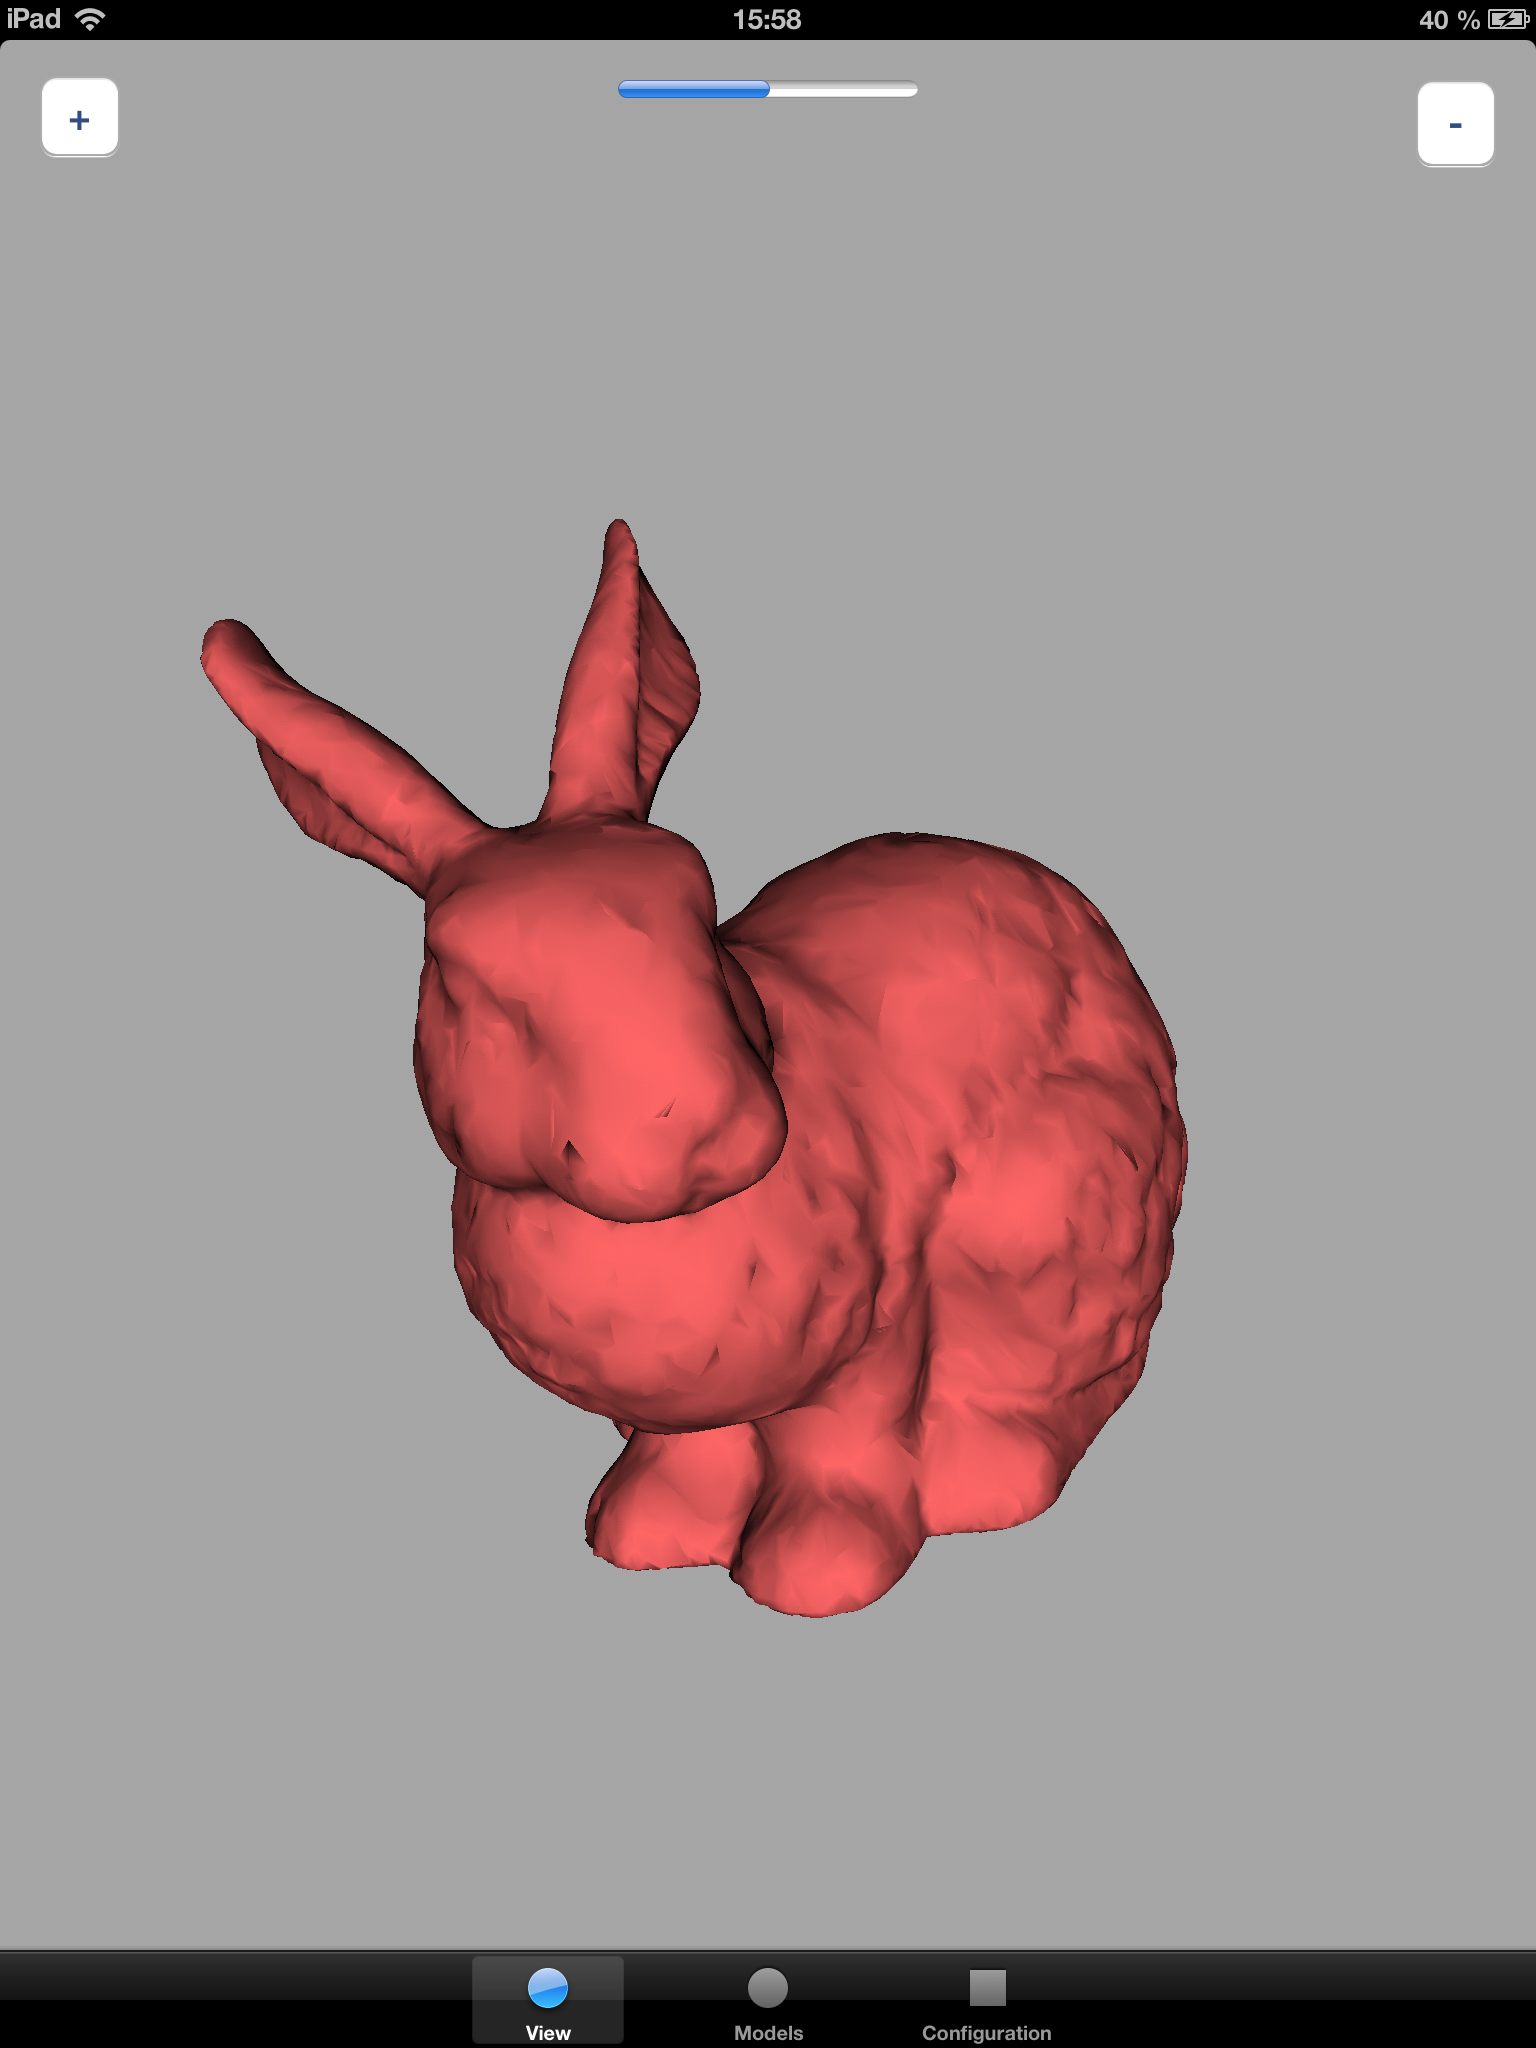
\includegraphics[width=1.0\textwidth]{images/ModelView.png}
	\caption{Screenshot of Model View Tab. There is a status bar on the top of the screen showing refinement process of current LOD}
	\label{fig:modelviewtab}
\end{figure}
\lstinputlisting[label=progmeshglkviewcrtl,caption=ProgMeshGLKViewController.h, style=Xcode, firstline=4, lastline=14]{codes/uiimpl.m}
\FG{fig:modelviewtab} shows the \textbf{Model View} tab of client application on iPad. The Model View tab is implemented using 
\texttt{ProgMeshGLKViewController}, which is subclass of \texttt{GLKViewController} (See Listing~\ref{progmeshglkviewcrtl}). It is mainly responsible for user interaction and rendering the model scene on iPad's screen. 

\subsection{Model List Tab}
\label{section:modellist}
\begin{figure}
	\centering
	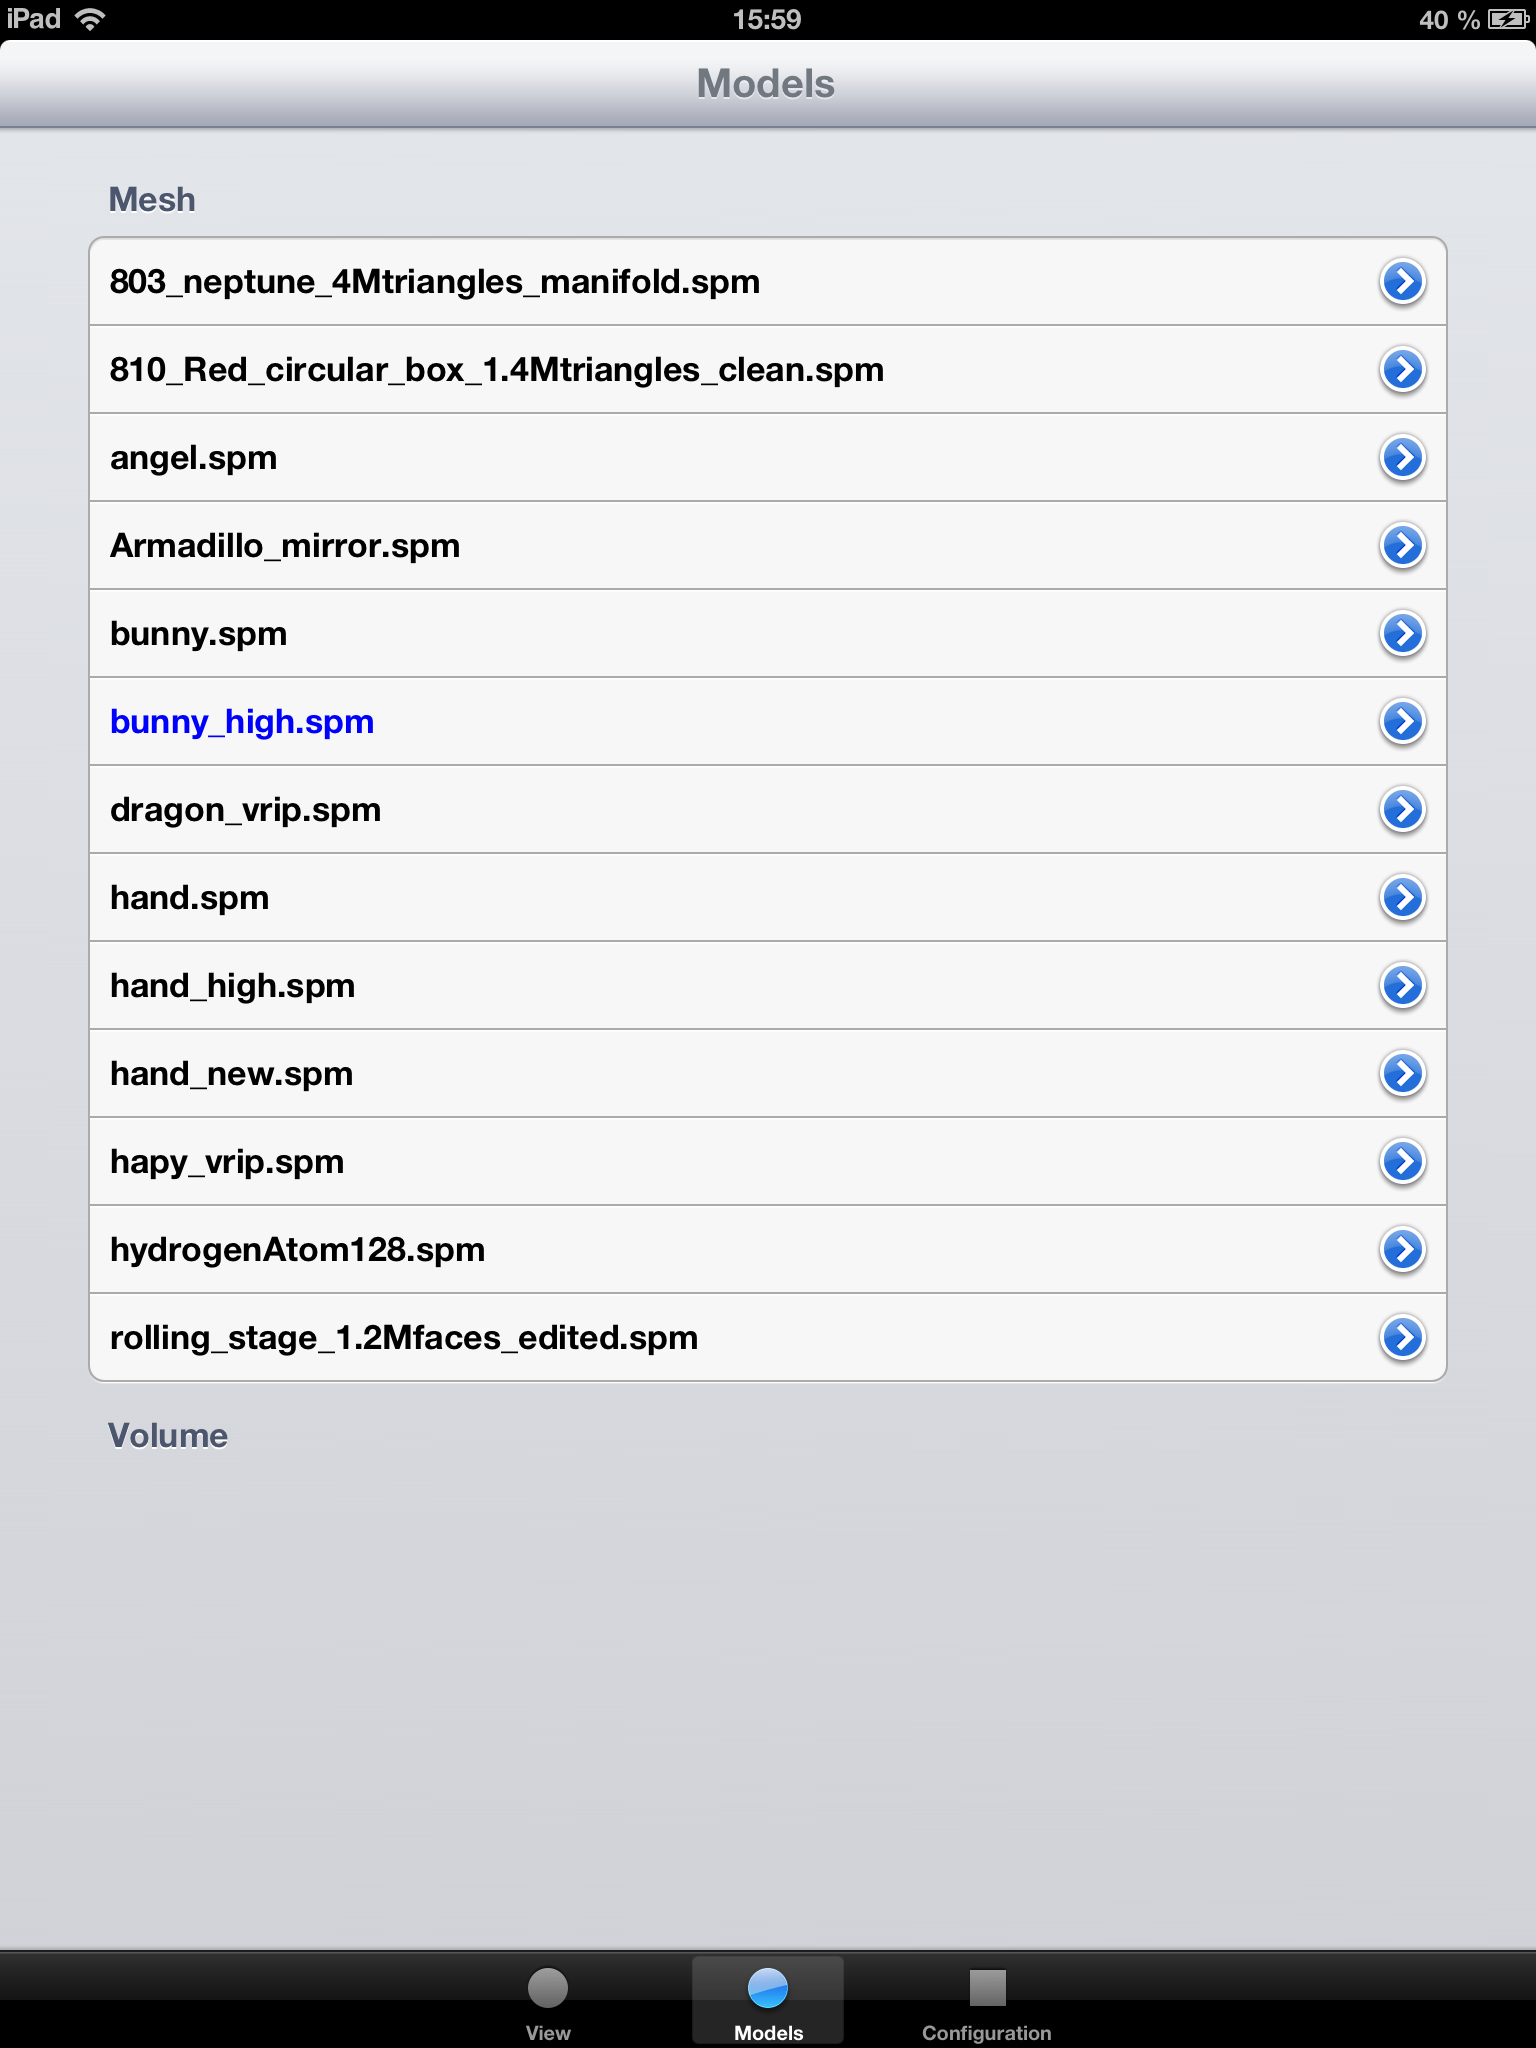
\includegraphics[width=1.0\textwidth]{images/ModelList.png}
	\caption{Screenshot of Model List Tab.}
	\label{fig:modellisttab}
\end{figure}
\lstinputlisting[label=progmeshmodeltableviewctl,caption=ProgMeshModelTableViewController.h, style=Xcode, firstline=17, lastline=24]{codes/uiimpl.m}

The second tab is the \textbf{Model List} tab, as showed in \FG{fig:modellisttab}. It has a list of all currently available models in the mesh repository on the server. When a user picks any item in the list, there will be background thread trying to load the bash mesh of the selected model from server. This tab is implemented using \texttt{ProgMeshModelTableViewController} which extends the base class \texttt{UITableViewController} provided by the iOS system itself (See Listing~\ref{progmeshmodeltableviewctl}). 


\subsection{Configuration Tab}
\label{section:configuration}

\begin{figure}
\centering
\subfigure[b][Configuration tab (disconnected)]{
	\centering
	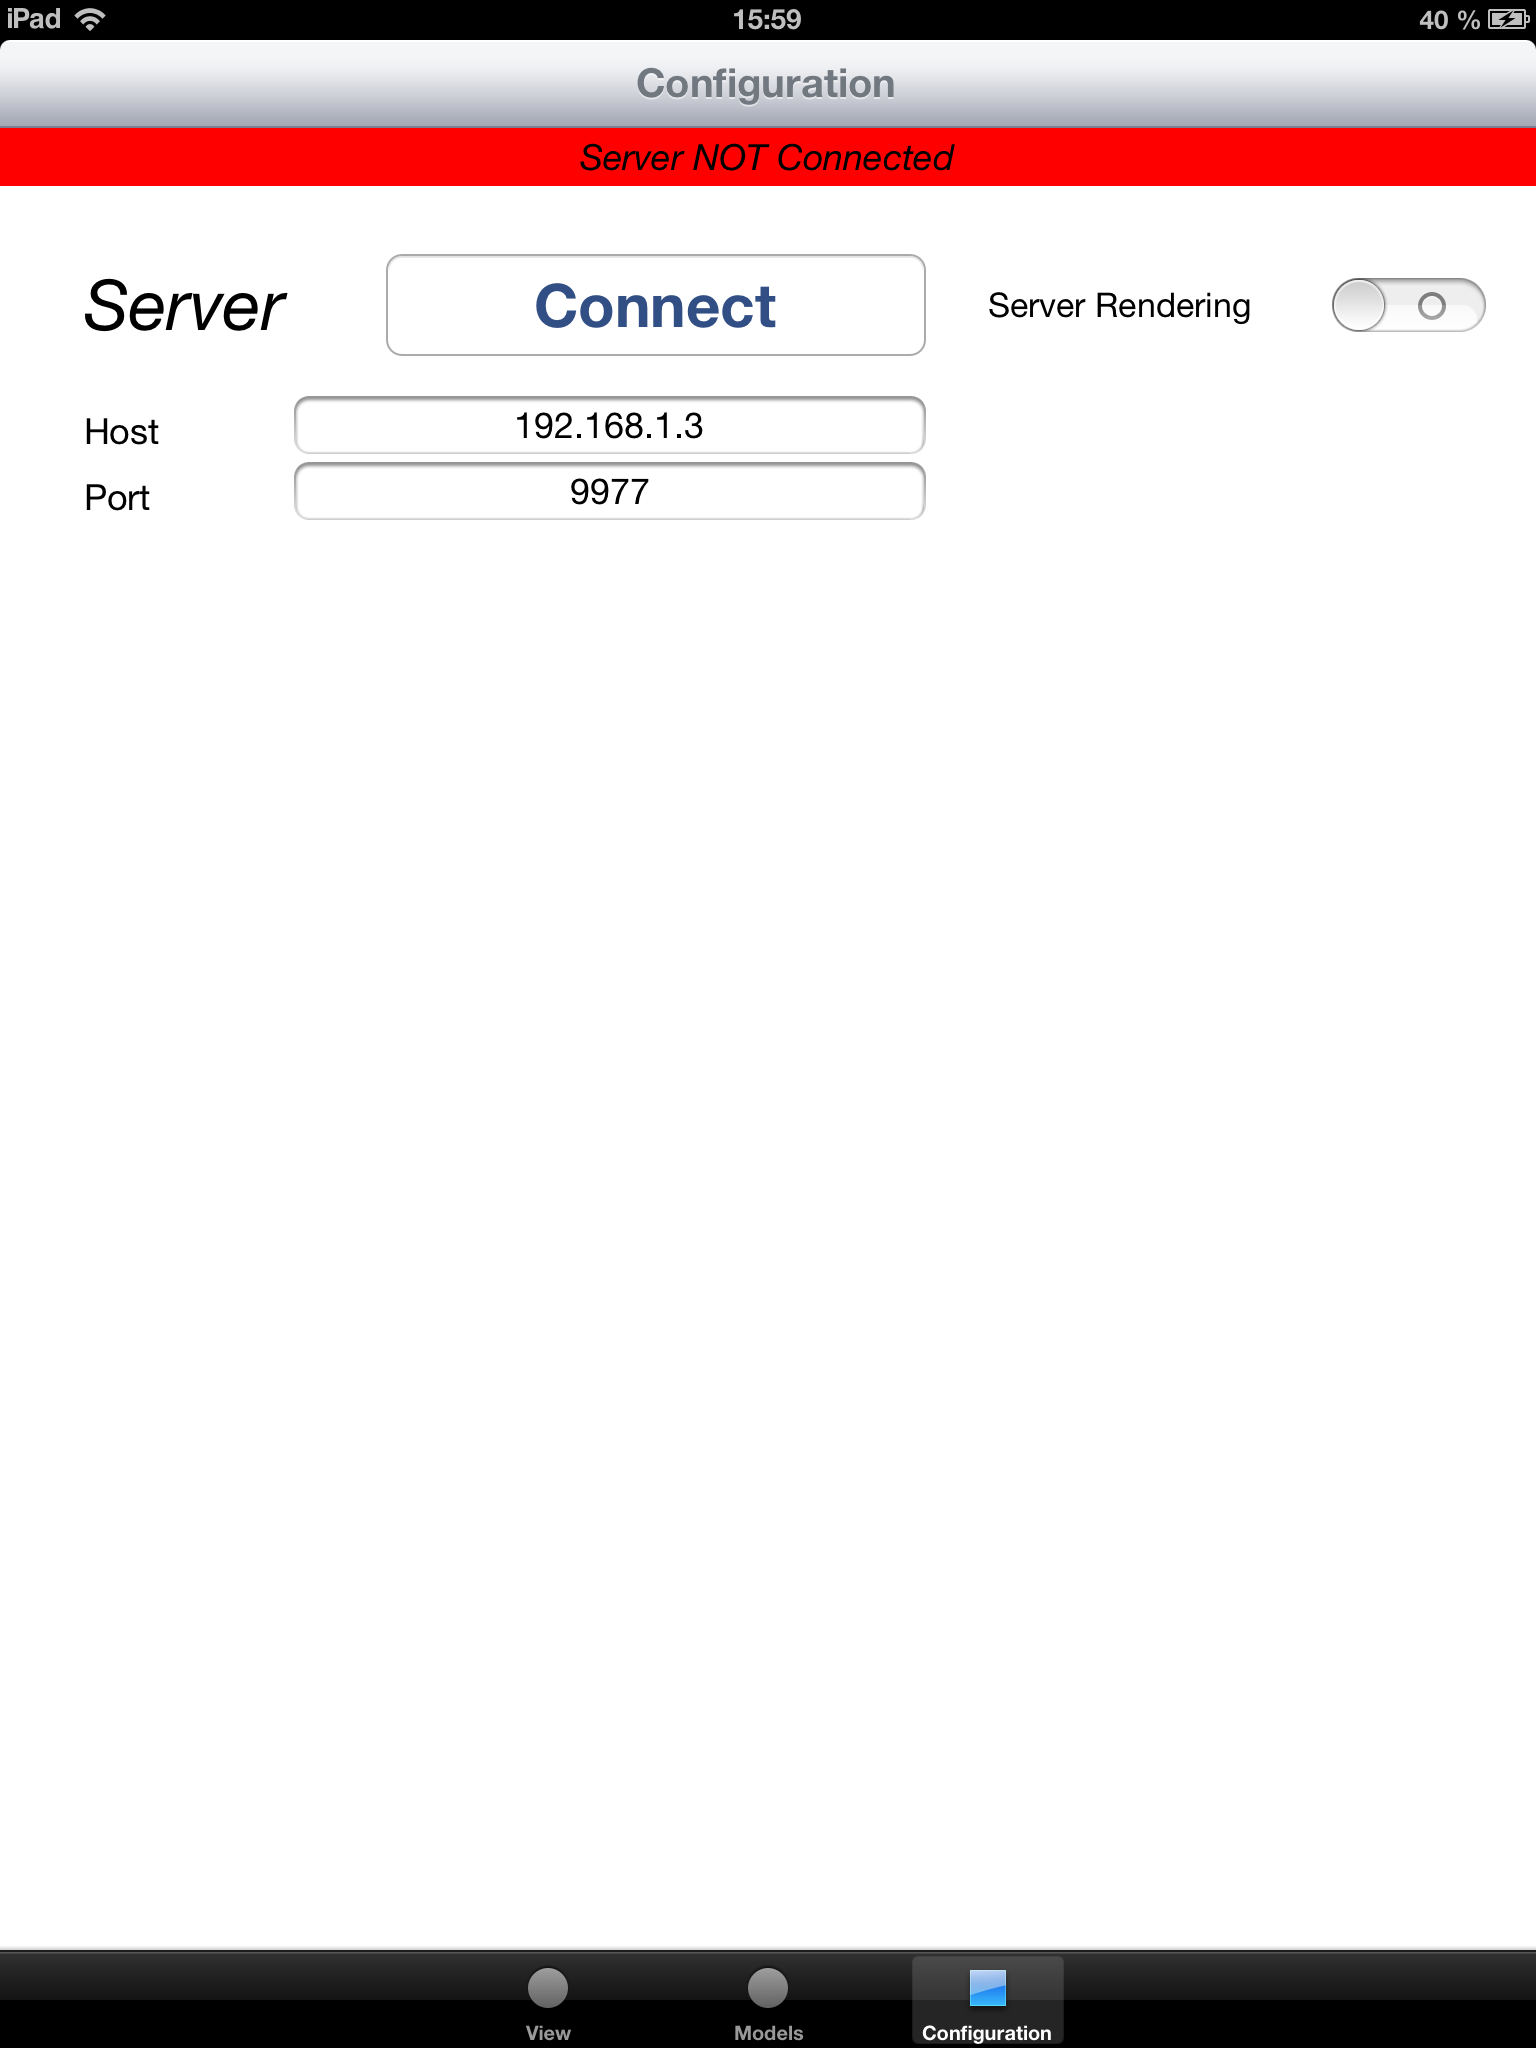
\includegraphics[width =0.45\textwidth] {images/ConfigurationDisconnected.png}
	\label{fig:configtab:disconnected}
}
\hfill
\subfigure[b][Configuration tab (connected)]{
	\centering
	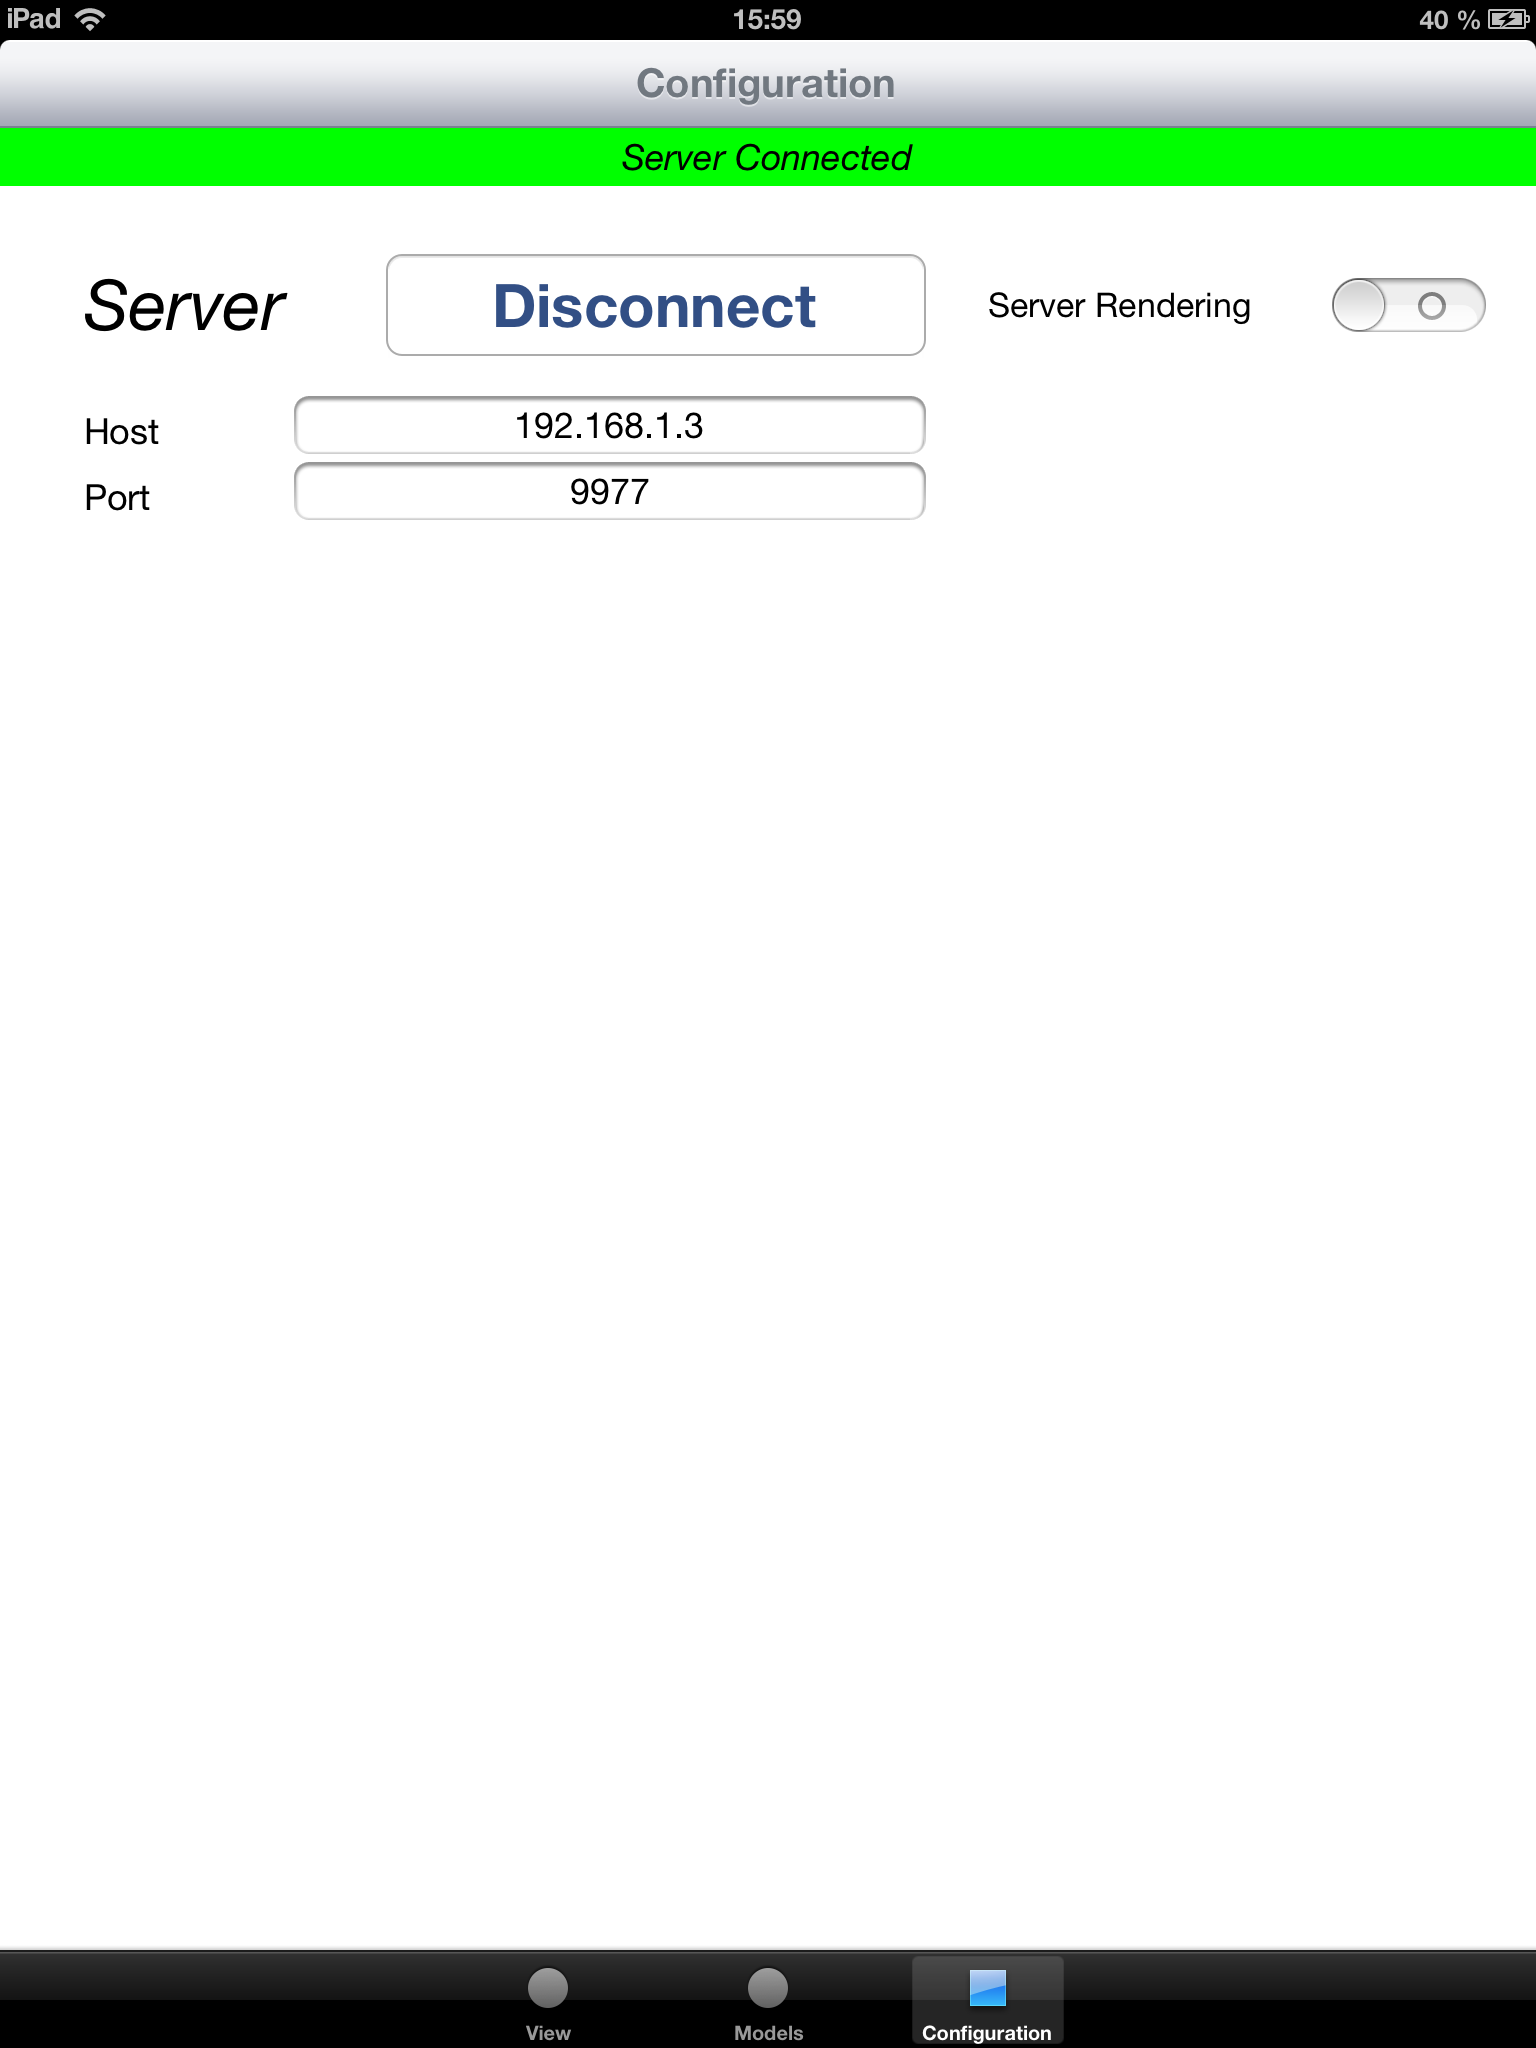
\includegraphics[width =0.45\textwidth] {images/ConfigurationConnected.png}
	\label{fig:configtab:connected}
}
\label{fig:configtab}
\caption{Screenshot of Configuration Tab}
\end{figure}
The last tab, \textbf{Configuration} tab, provides graphics interface to user for the configuration of server IP address, port, control of connection and switching of rendering mode (client/server rendering), as showed in \FG{fig:configtab:disconnected} and \FG{fig:configtab:connected}. It is implemented using class \texttt{ConfigViewController} which is a subclass of \texttt{UIViewController} (See Listing~\ref{configviewcode}). \\

\noindent
\begin{minipage}{\linewidth}
\makebox[\linewidth]{
\lstinputlisting[label=configviewcode,caption=ConfigViewController.h, style=Xcode, firstline=27, lastline=37]{codes/uiimpl.m}
}
\bigskip
\end{minipage}


%\section{Implementation Discussion}
%\TODO{Discussion on implementation. }

%Picture
%\noindent
%\begin{minipage}{\linewidth}
%\makebox[\linewidth]{%
%\includegraphics[width=1.0\textwidth]{images/morphable.pdf}}
%\captionof{figure}{MorphableUI generates user-tailored interfaces for arbitrary applications in arbitrary environments. Users are able to use all available devices to control as many applications as needed. User behavior is analyzed by the system to increase the user experience.}% only if needed
%\label{fig:morphable}
%\bigskip
%\end{minipage}



\chapter{Evaluation}
\label{chapter:result}
%\TODO{In this chapter, we will describe the evaluation methodology and experimental results of our system. }
The main contribution of this thesis work is the view-dependent progressive mesh streaming framework on iPad. We have described and illustrated the design and implementation details of our system in previous chapters. In this chapter, we will do some experiment on our system and illustrate the evaluation results.  

\section{Overview}
\label{chapter:result:overview}
Since our framework provides both client and server rendering of progressive mesh, experiments are performed both for client rendering and server rendering scenario. The initial purpose of providing two ways of rendering is to process large models which are not suitable for client rendering, therefore different models will be used to test the system's performance in both scenarios. 
\subsection{Models for Test}
\label{chapter:result:overview:modelfortest}
Below is a list of test models: 
\begin{table}
\begin{center}
    \begin{tabular}{|	p{7.5cm}	|	l	|	l	|}
    \hline
    	\textbf{Model Name} 							& \textbf{Num. Vertices} 	& \textbf{Num. Faces}	\\ \hline
	bunny								&2503			&4968		\\ \hline
	bunny\_high							&34834			&69664		\\ \hline
	Armadillo\_mirror						&172974			&345944		\\ \hline
	hand									&210528			&416384		\\ \hline
	angel								&237018			&474048		\\ \hline
	hand\_new							&327323			&654666		\\ \hline
	dragon\_vrip							&437645			&871414		\\ \hline
    \end{tabular}
    \caption{Test models for client rendering.}
    \label{table:modelsclientrendering}
\end{center}
\end{table}

\begin{table}
\begin{center}
    \begin{tabular}{|	p{7.5cm}	|	l	|	l	|}
    \hline	
    	\textbf{Model Name} 						& \textbf{Num. Vertices} 	& \textbf{Num. Faces}	\\ \hline
    	happy\_vrip							&543652			&1087716		\\ \hline
	rolling\_stage\_1.2Mfaces\_edited			&596903			&1192501		\\ \hline
	810\_Red\_circular\_box\_1.4Mtriangles\_clean	&701332			&1402640		\\ \hline
	803\_neptune\_4Mtriangles\_manifold		&2003932			&4007872		\\ \hline
	Thai Statue							&5000000			&10000000	\\ \hline
    \end{tabular}
    \caption{Test models for server rendering.}
    \label{table:modelsserverrendering}
\end{center}
\end{table}

\TA{table:modelsclientrendering} lists test models for client rendering and \TA{table:modelsserverrendering} lists test models for server rendering. Models for both situations are sorted according to number of vertices and faces they contain. Here we decide to do server rendering for models with over 1M faces. 

\subsection{Hardware Setup}
%\TODO{This section describes hardwares we used for experiments. }\\
Since our framework is a client-server based application, we will illustration the hardware setup of both client and server side. \\

The \textbf{Client} side application is implemented and deployed on an \textbf{iPad 3rd generation\footnote{\label{ipad3rd}\url{http://support.apple.com/kb/SP647}}}. It has a Dual-core Apple A5X CPU (ARMv7) clocked at 1 GHz, with a system-on-chip quad-core graphics processor and 1 GB RAM. Its operating system is iOS 6.1.3. \\

And the \textbf{Server} side application is implemented and deployed on a \textbf{Macbook} with a Intel Core 2 Duo CPU of 2.4 GHz and 4 GB of DDR3 RAM. The server side operating system is MAC OS X 10.8.3. \\

The \textbf{Network Environment} we experiment in is a 10/100 M WiFi network environment with average roundtrip delay of 30.569 ms

\section{Experiment Results }
\label{section:expresult}
We evaluate our framework separately for server and client rendering scenario. And for each scenario, we measure our framework in three aspects: (1) Transmission Performance, (2) Memory/CPU Usage and (3) Visual Quality. \\

A standard testing process is defined. For each experiment, we will first open the model to test. (As default it will be put in the center of screen. ) Next we start the streaming process until maximum LOD is reached. And then we rotate to the back side and zoom-in to the center-part of the model. The test ends until maximum LOD is reached in current viewing situation. In the following sections we will illustrate the evaluation results of our experiments. 

\subsection{Client Rendering Evaluation}
\label{section:clienteva}
The client rendering evaluation experiments are performed on the models listed in \TA{table:modelsclientrendering}. 
\subsubsection{Transmission Performance}
\label{section:clienttransperf}
\begin{figure}[htb]
	\centering
	
	\begin{pdfpic}
\psline[linewidth=0.05cm,arrowsize=0.05291667cm 2.32,arrowlength=1.4,arrowinset=0.4]{->}(0.38910156,3.9910352)(0.38910156,-4.508965)
\usefont{T1}{ptm}{m}{n}
\rput(2.1228712,4.396035){Client}
\usefont{T1}{ptm}{m}{n}
\rput(5.5489354,4.396035){Server}
\psline[linewidth=0.02cm,linestyle=dashed,dash=0.16cm 0.16cm](2.0891016,4.1910353)(2.0891016,-4.508965)
\psline[linewidth=0.02cm,linestyle=dashed,dash=0.16cm 0.16cm](5.589102,4.1910353)(5.589102,-4.508965)
\usefont{T1}{ptm}{m}{n}
\rput{-90.0}(0.3924024,7.245801){\rput(3.7567968,3.651035){\Huge ...}}
\psline[linewidth=0.04cm,arrowsize=0.05291667cm 2.0,arrowlength=1.4,arrowinset=0.4]{->}(2.3891015,2.5910351)(5.2891016,2.0910351)
\usefont{T1}{ptm}{m}{n}
\rput{-8.649829}(-0.34278482,0.62180525){\rput(3.9170704,2.5960352){SyncViewingParam}}
\psline[linewidth=0.04cm,arrowsize=0.05291667cm 2.0,arrowlength=1.4,arrowinset=0.4]{<-}(2.5293014,0.5025208)(5.248902,1.2795495)
\usefont{T1}{ptm}{m}{n}
\rput{16.396927}(0.4885742,-1.0360752){\rput(3.8367383,1.1960351){VsplitStream}}
\psframe[linewidth=0.04,dimen=outer,fillstyle=solid](5.7891016,2.0910351)(5.3891015,1.1910352)
\usefont{T1}{ptm}{m}{n}
\rput(6.6628613,1.6960351){Processing}
\psframe[linewidth=0.04,dimen=outer,fillstyle=solid](2.2891016,0.29103515)(1.8891015,-0.60896486)
\usefont{T1}{ptm}{m}{n}
\rput(3.5271094,-0.10396484){Refine&Render}
\psframe[linewidth=0.04,dimen=outer,fillstyle=solid](2.2891016,-1.1089648)(1.8891015,-2.4089649)
\usefont{T1}{ptm}{m}{n}
\rput(3.4667382,-1.4039649){ViewingParam}
\psline[linewidth=0.05cm,arrowsize=0.05291667cm 2.32,arrowlength=1.4,arrowinset=0.4]{->}(2.0891016,-0.60896486)(2.0891016,-1.1089648)
\usefont{T1}{ptm}{m}{n}
\rput(3.0408204,-1.7039648){Decrease}
\psline[linewidth=0.04cm,arrowsize=0.05291667cm 2.0,arrowlength=1.4,arrowinset=0.4]{->}(2.2891016,-2.2089648)(5.4891014,-2.8089647)
\usefont{T1}{ptm}{m}{n}
\rput{-8.649829}(0.45317224,0.5464833){\rput(3.8170702,-2.703965){SyncViewingParam}}
\psframe[linewidth=0.04,dimen=outer,fillstyle=solid](5.7891016,-2.7089648)(5.3891015,-3.608965)
\usefont{T1}{ptm}{m}{n}
\rput{-90.0}(7.1924024,0.44580078){\rput(3.7567968,-3.148965){\Huge ...}}
\usefont{T1}{ptm}{m}{n}
\rput(0.35844725,4.396035){Time}
\usefont{T1}{ptm}{m}{n}
\rput(9.480206,1.4960351){Elapsed Time}
\psline[linewidth=0.04cm,arrowsize=0.05291667cm 2.0,arrowlength=1.4,arrowinset=0.4]{->}(7.7891016,0.99103516)(8.389102,1.3910352)
\usefont{T1}{ptm}{m}{n}
\rput{-90.0}(8.092402,-0.45419908){\rput(3.7567968,-4.048965){\Huge ...}}
\psframe[linewidth=0.04,dimen=outer,fillstyle=solid](2.2891016,3.5910351)(1.8891015,2.2910352)
\psframe[linewidth=0.05,linestyle=dashed,dash=0.16cm 0.16cm,framearc=0.25,dimen=outer](7.6891017,3.1910353)(1.3891015,-0.9089649)

	\end{pdfpic} 
	\caption{Client Rendering Transmission Elapsed Time Illustration}
	\label{fig:clientrndtransillu}

\end{figure}
\begin{figure}
\centering
\subfigure[b][Data Transmission. X Axis: time (second), Y Axis: Data (KB).]{
	\centering
	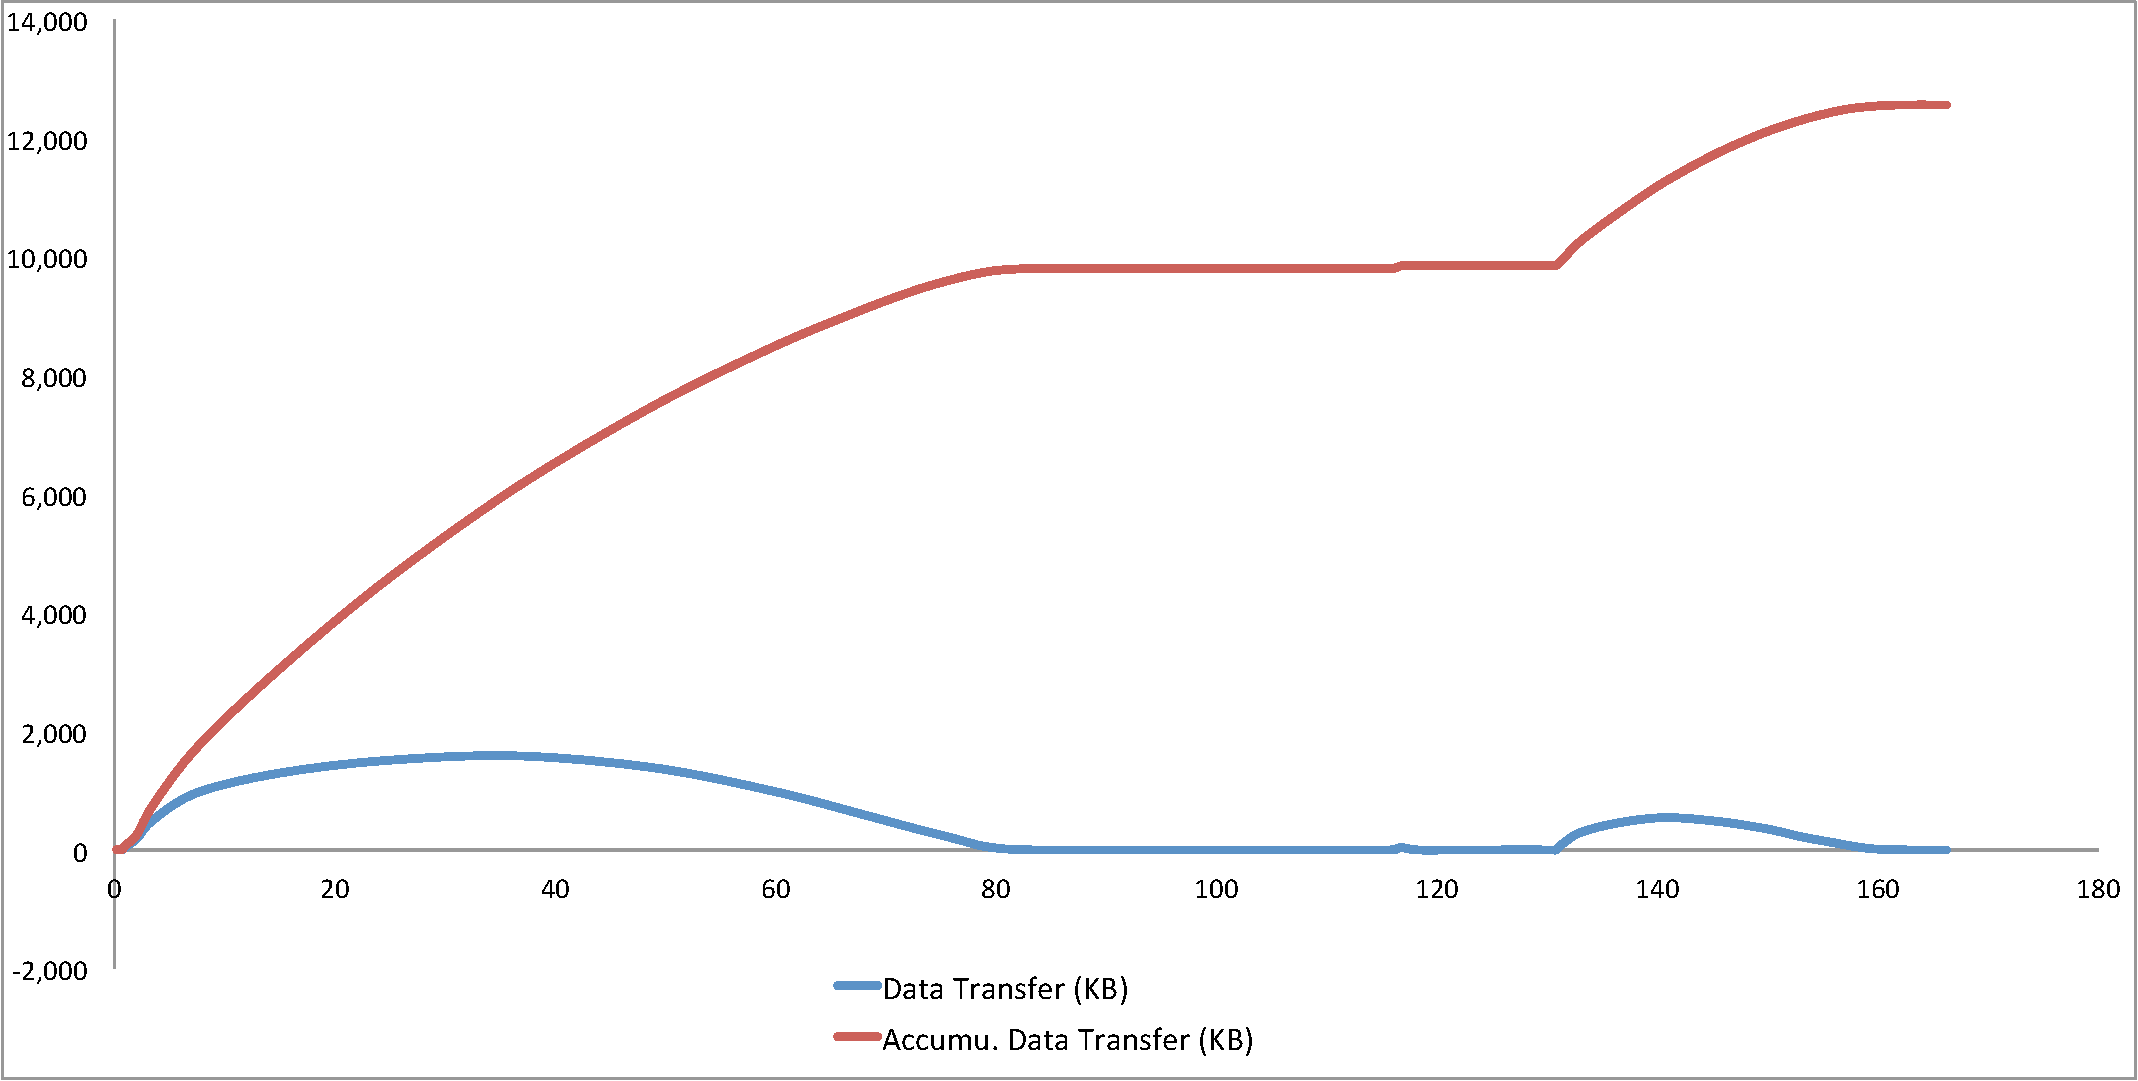
\includegraphics[width =\textwidth] {results/hand_trans_perf.pdf}
	\label{fig:hand_trans_perf_data}
}
\subfigure[b][Elapsed Time of each Viewing Parameter Synchronization. X Axis: Sync Request, Y Axis: Elapsed Time (second)]{
	\centering
	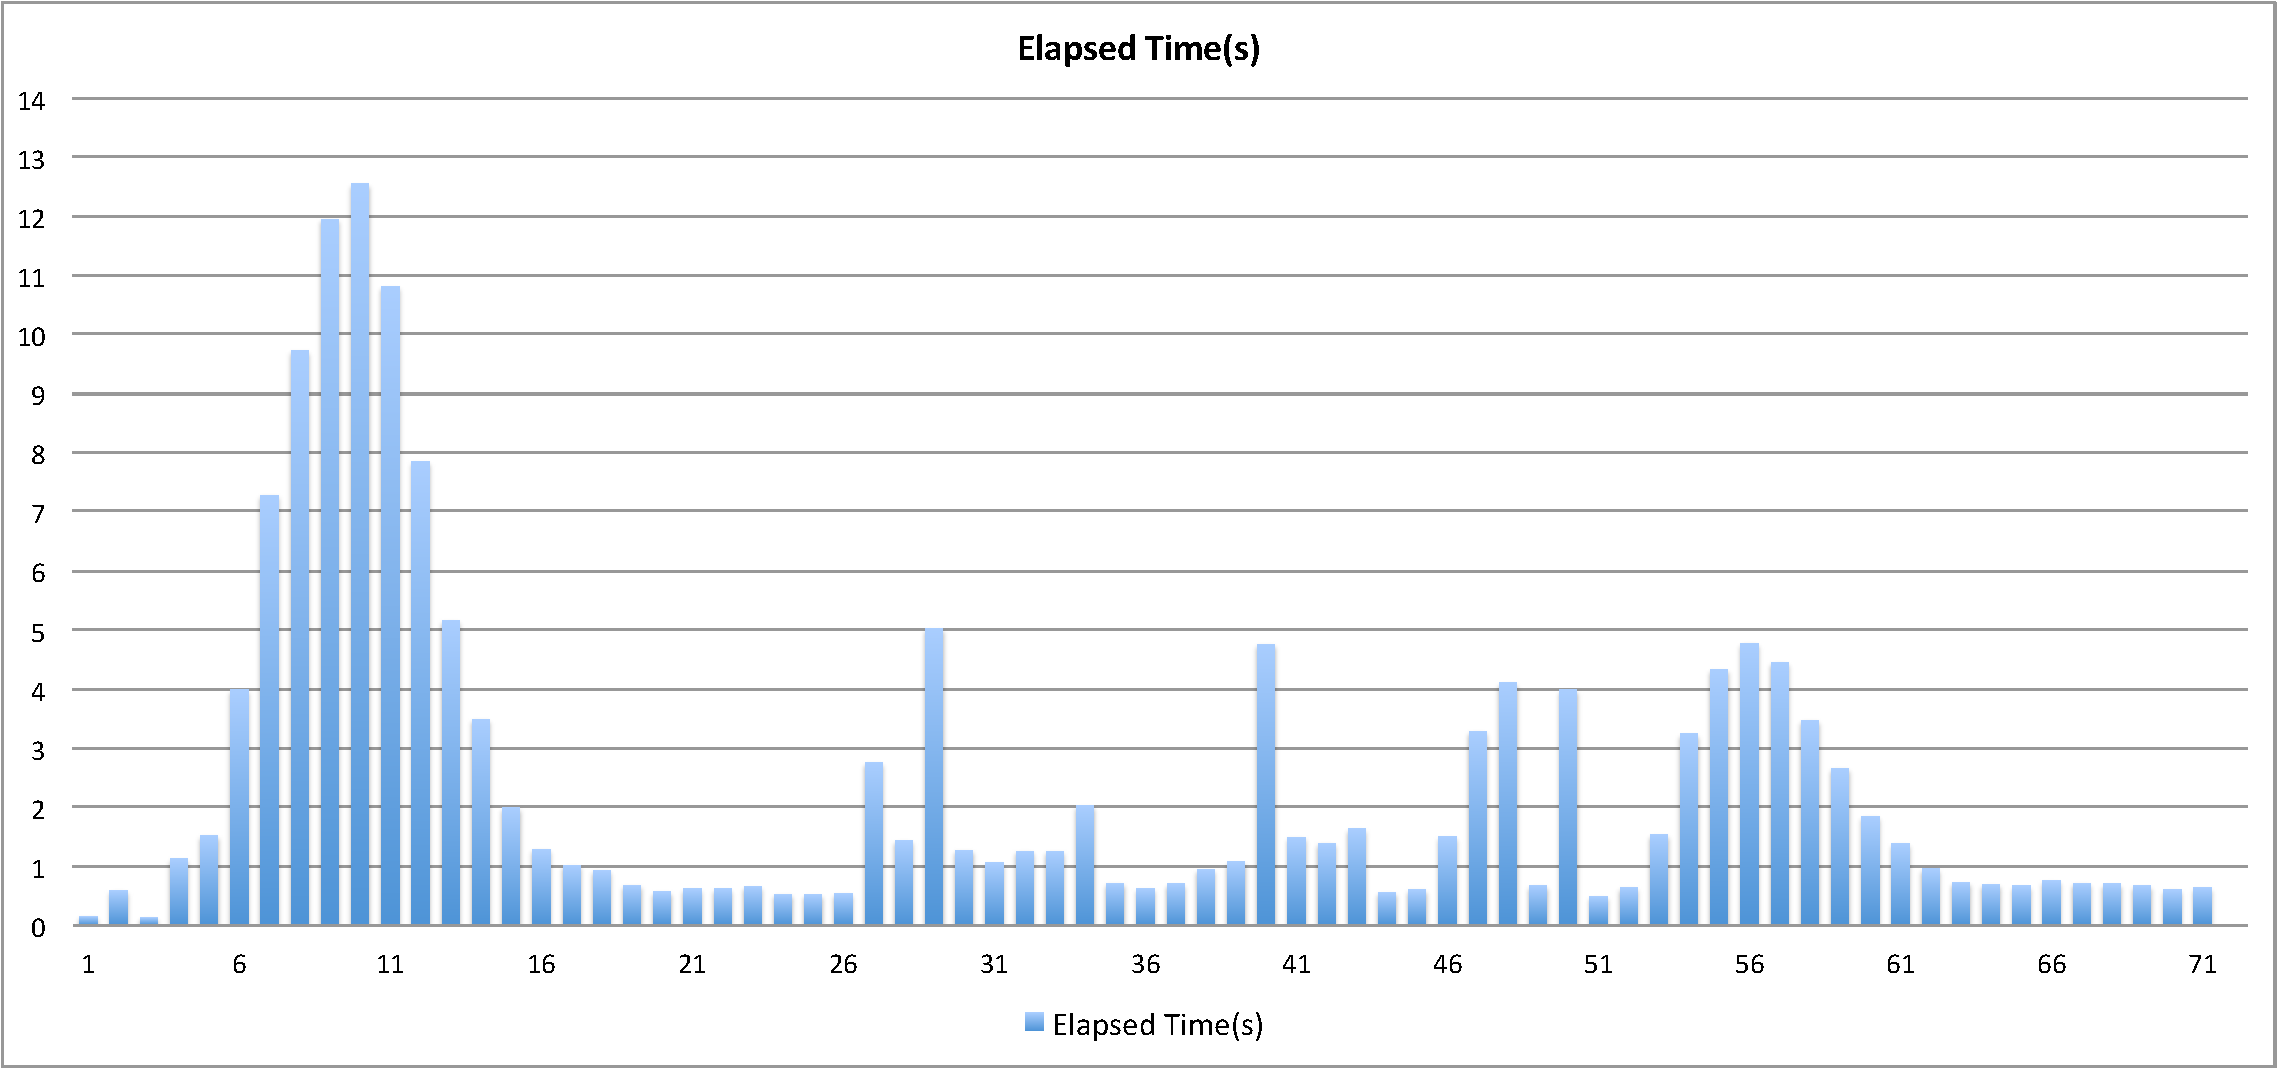
\includegraphics[width =\textwidth] {results/hand_trans_perf_elapsed_time.pdf}
	\label{fig:hand_trans_perf_elapsedtime}
}
\label{fig:hand_trans_perf}
\caption{Client Rendering Data Transmission Performance of Model "hand"}
\end{figure}

\begin{figure}
\centering
\subfigure[b][Data Transmission. X Axis: time (second), Y Axis: Data (KB).]{
	\centering
	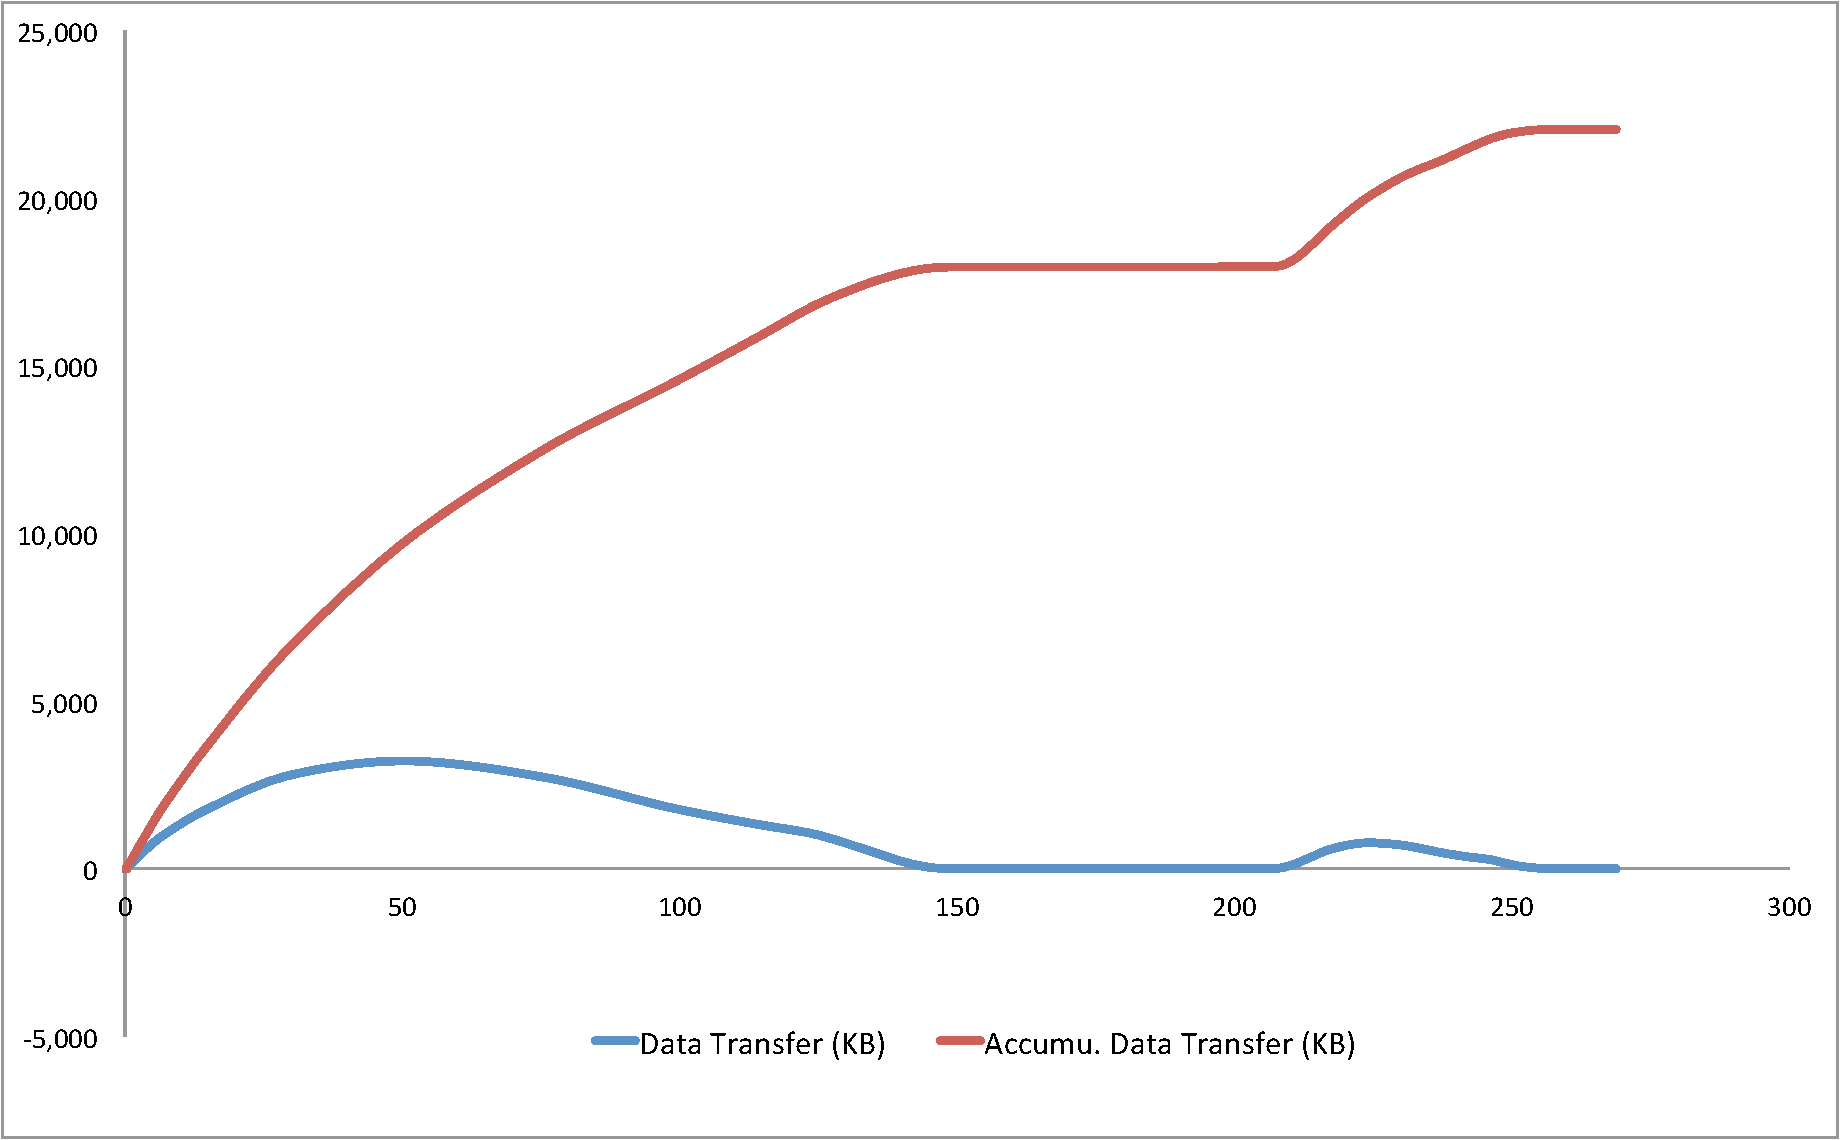
\includegraphics[width =\textwidth] {results/dragon_vrip_trans_perf.pdf}
	\label{fig:dragon_vrip_trans_perf_data}
}
\subfigure[b][Elapsed Time of each Viewing Parameter Synchronization. X Axis: Sync Request, Y Axis: Elapsed Time (second)]{
	\centering
	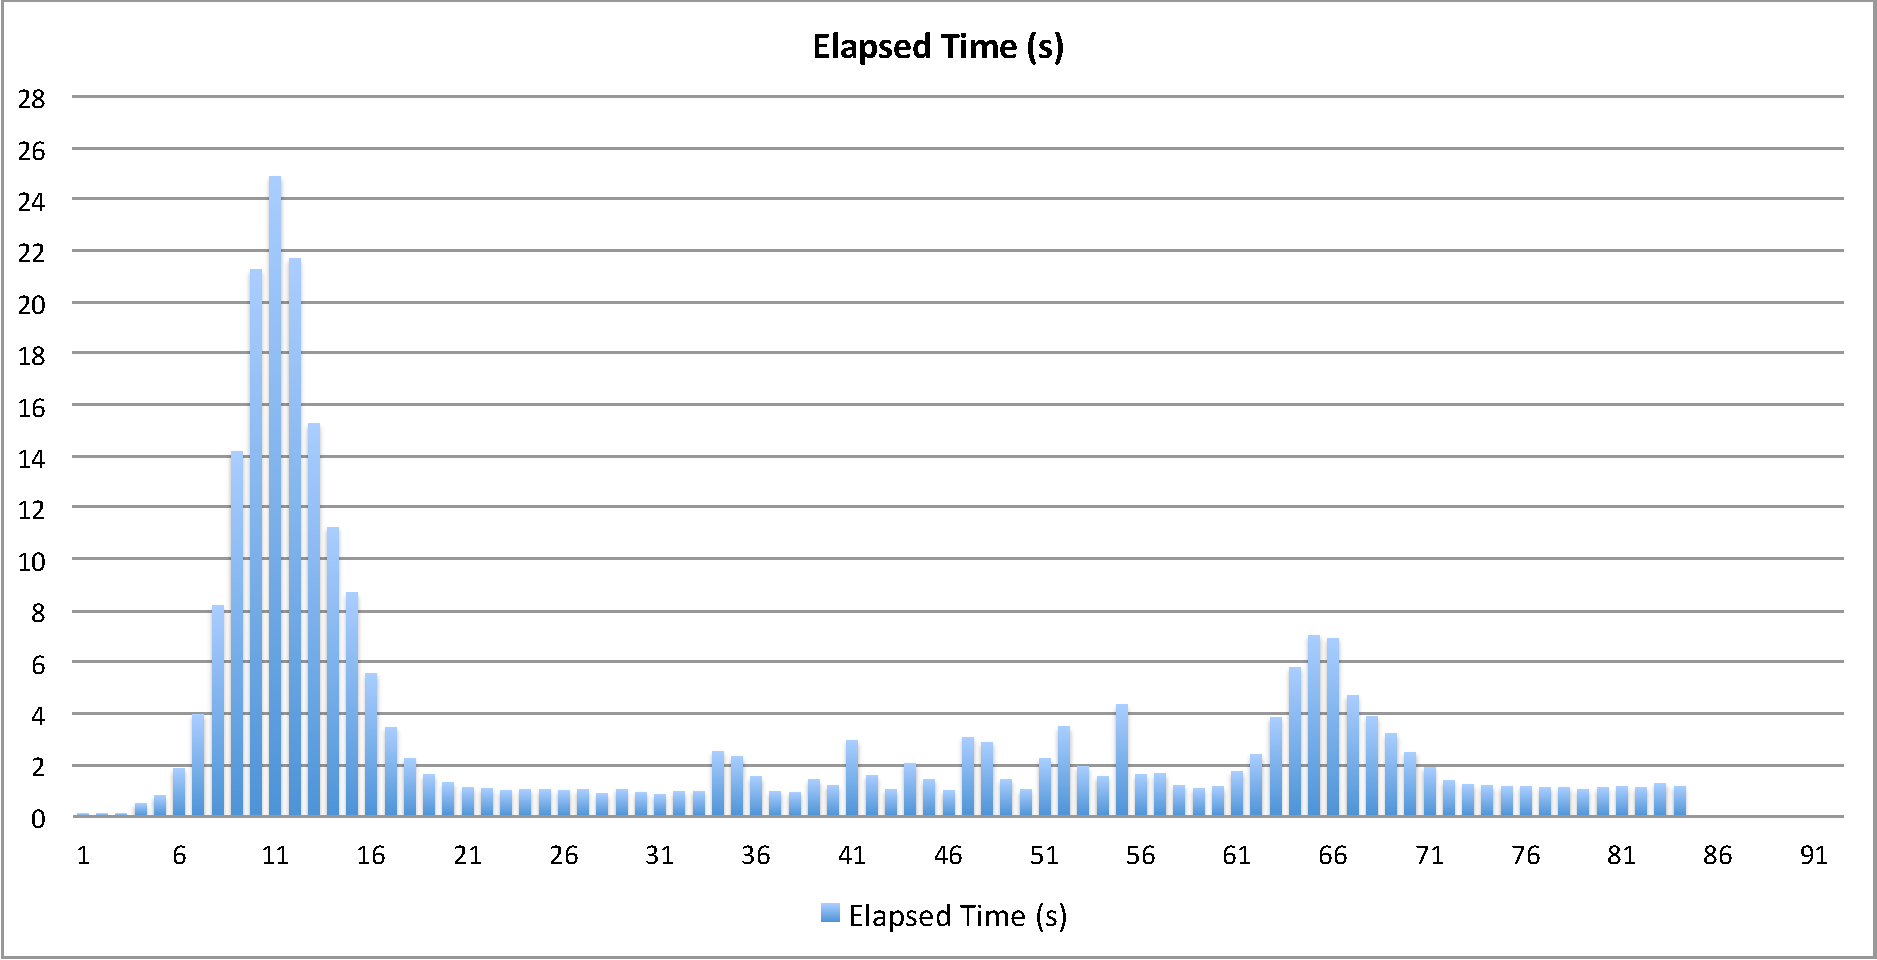
\includegraphics[width =\textwidth] {results/dragon_vrip_trans_perf_elapsed_time.pdf}
	\label{fig:dragon_vrip_trans_perf_elapsedtime}
}
\label{fig:dragon_vrip_trans_perf}
\caption{Client Rendering Data Transmission Performance of Model "dragon\_vrip"}
\end{figure}


Recall the transmission process in the situation of client rendering. When a connection is established and there is no more user interaction on client's screen, the client application will repeatedly reduce the screen error tolerance by half and send the viewing  parameter with updated screen error tolerance to server for new $vsplit$ packets. Then $vsplit$ packets corresponding to current viewing parameter are transmitted to client and the client will perform refinement operation on current mesh. Once the refinement is finished, if there's no more user interaction,  the client will continue to decrease the screen error tolerance and perform the process again until current possible maximum LOD is reached. Therefore, we collect the elapsed time and $vsplit$ packet's size for each viewing parameter synchronization and response process. \FG{fig:clientrndtransillu} illustrates each sampled elapsed time interval. \\

\FGp{fig:hand_trans_perf_data} shows the data transmission performance experiment we performed on model "hand" (See \TAp{table:modelsclientrendering}). The X axis denotes the time passed and the Y axis denotes the data amount in the unit of KB. The blue curve illustrates the data transfer amount upon each viewing parameter synchronization request. And the red curve illustrates the accumulative data transfer amount over the time. It can be discovered that the major data transmission occurs between 0 - 80 seconds and 130 - 160 seconds. It is easy to explain: in the first 80 seconds we are streaming from the initial view of the model. And next crest reflects the rotation of view and the streaming process of model's back side geometry. During 80 - 130 seconds we are interacting with the model to adjust it to the second viewing angle and scale. From \FGp{fig:hand_trans_perf_data} we can also get the time of streaming from base mesh to highest LOD with maximum details for a specific viewing parameter with the model "hand". For the initial one it costs about 80 seconds. And for the second one it costs about 30 seconds. The reason why this time is decreasing is that in the second phase we are viewing (and zooming into) a small area of the model's back center and it naturally contains less detail to refine. \\

\FGp{fig:hand_trans_perf_elapsedtime} shows the elapsed time for each viewing parameter sync request of the experiment on model "hand". The elapsed time includes network transmission time and client-side refine\&render time. Naturally it has similar trend of the blue line in \FGp{fig:hand_trans_perf_data}.







\subsubsection{Memory/CPU Usage}
\label{section:clientmemcpuusage}

\begin{figure}
\centering
\subfigure[b][CPU Usage]{
	\centering
	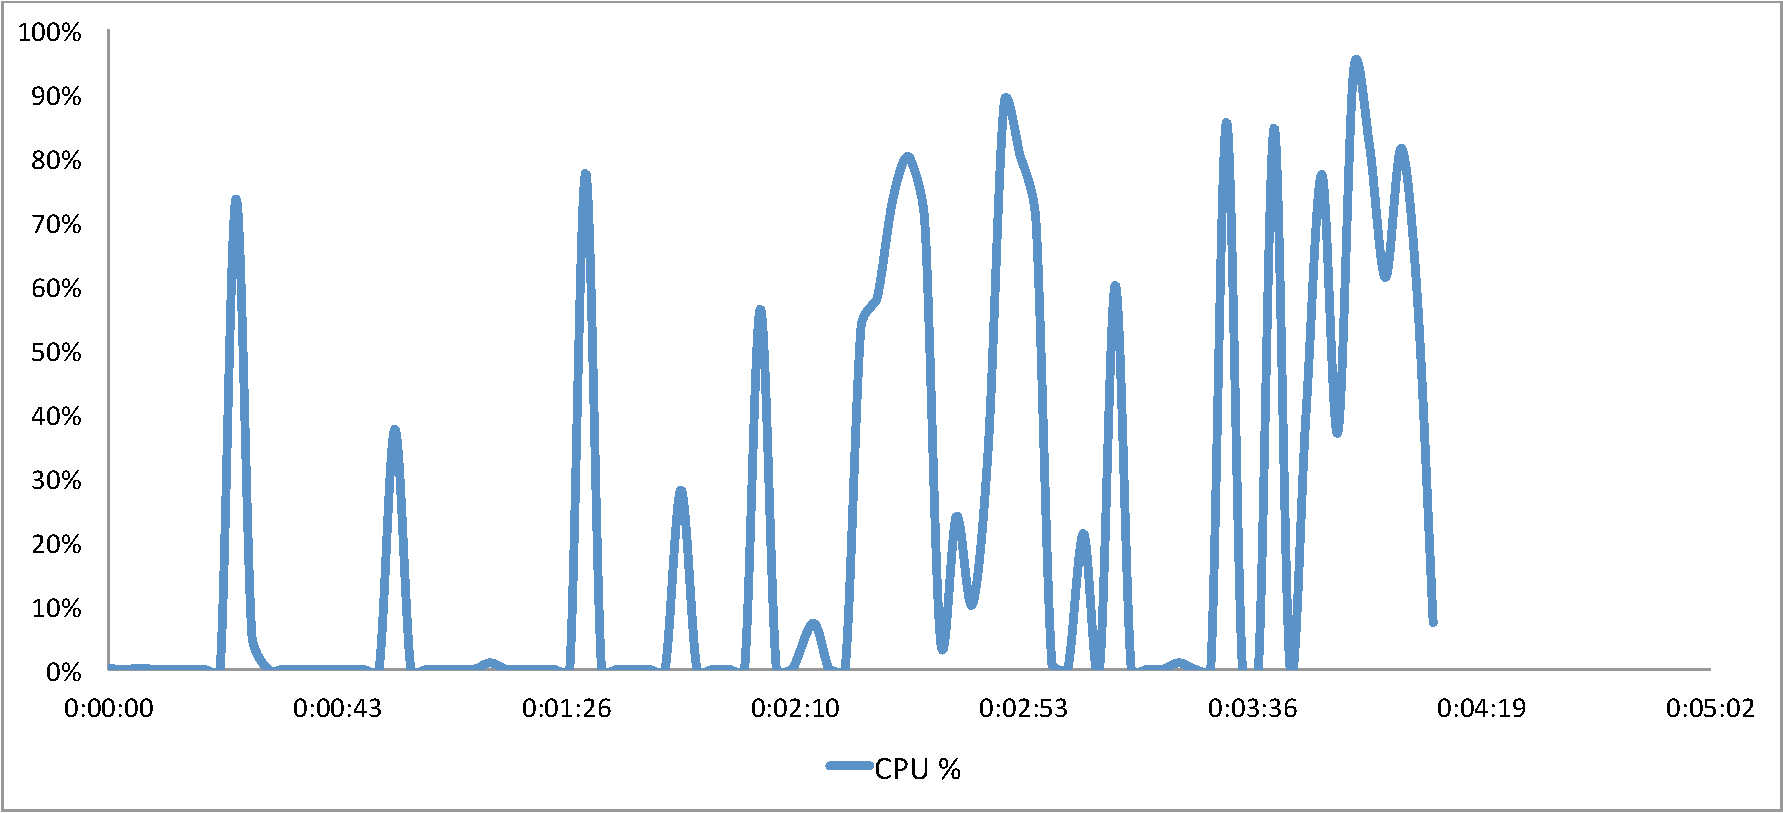
\includegraphics[width =\textwidth] {results/hand_new_cpu.pdf}
	\label{fig:hand_new_cpu}
}
\subfigure[b][Memory Usage]{
	\centering
	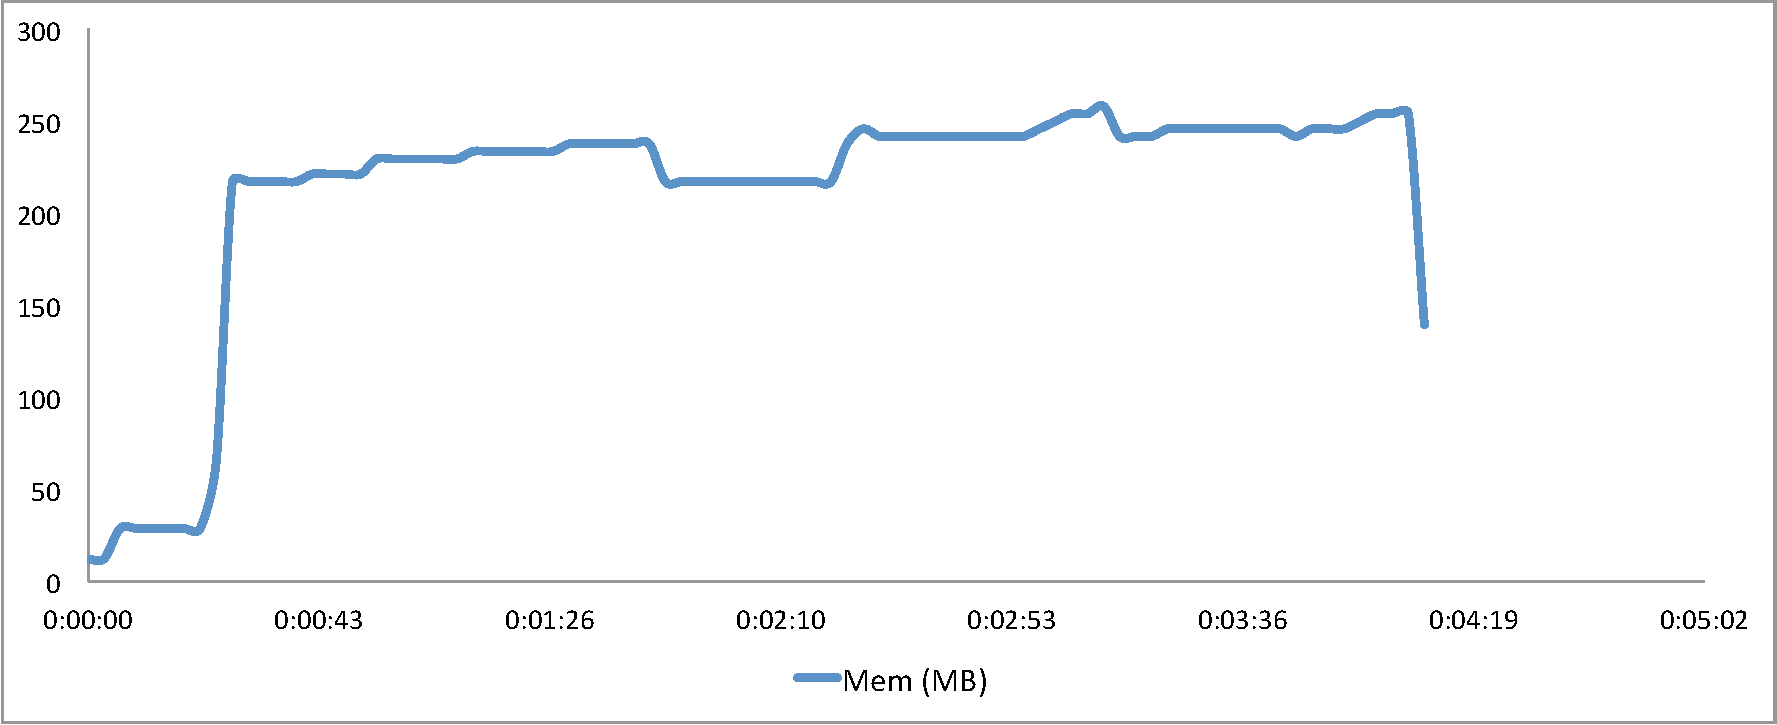
\includegraphics[width =\textwidth] {results/hand_new_mem.pdf}
	\label{fig:hand_new_mem}
}
\label{fig:hand_new_cpu_mem}
\caption{CPU and Memory Usage of Experiment on model "hand\_new"}
\end{figure}
We use model "hand\_new" for our Memory/CPU Usage experiment. \FG{fig:hand_new_cpu} illustrates the CPU usage from the beginning of streaming. During the experiment the model is rotated and zoomed in for different viewing angle and scale. We can see from it that there are a climax of CPU usage between each idle time, which is the effects of each server processing between two viewing parameter synchronization request from server. \FG{fig:hand_new_mem} shows the memory usage. It shows that the server's memory consumption is quite steady during streaming. 


\subsubsection{Visual Quality}
\label{section:clientvisualquality}
\begin{figure}
\centering
\subfigure[b][]{
	\centering
	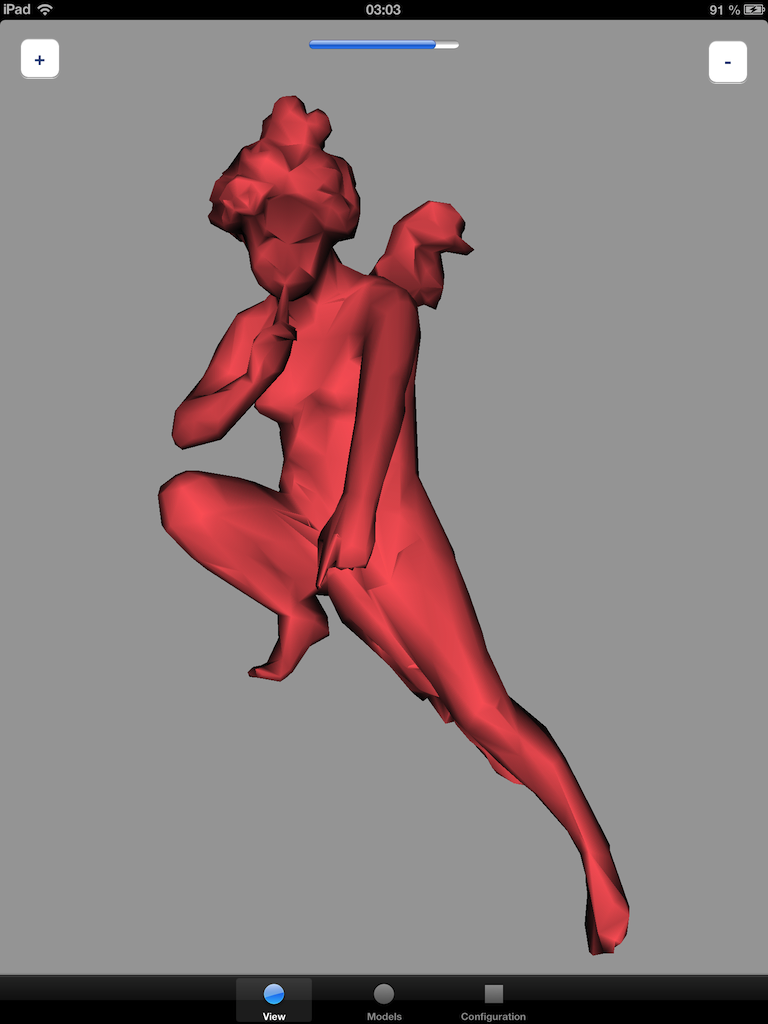
\includegraphics[width =0.45\textwidth] {results/030330.png}
	\label{fig:angel_visual_effects_1}
}
\hfill
\subfigure[b][]{
	\centering
	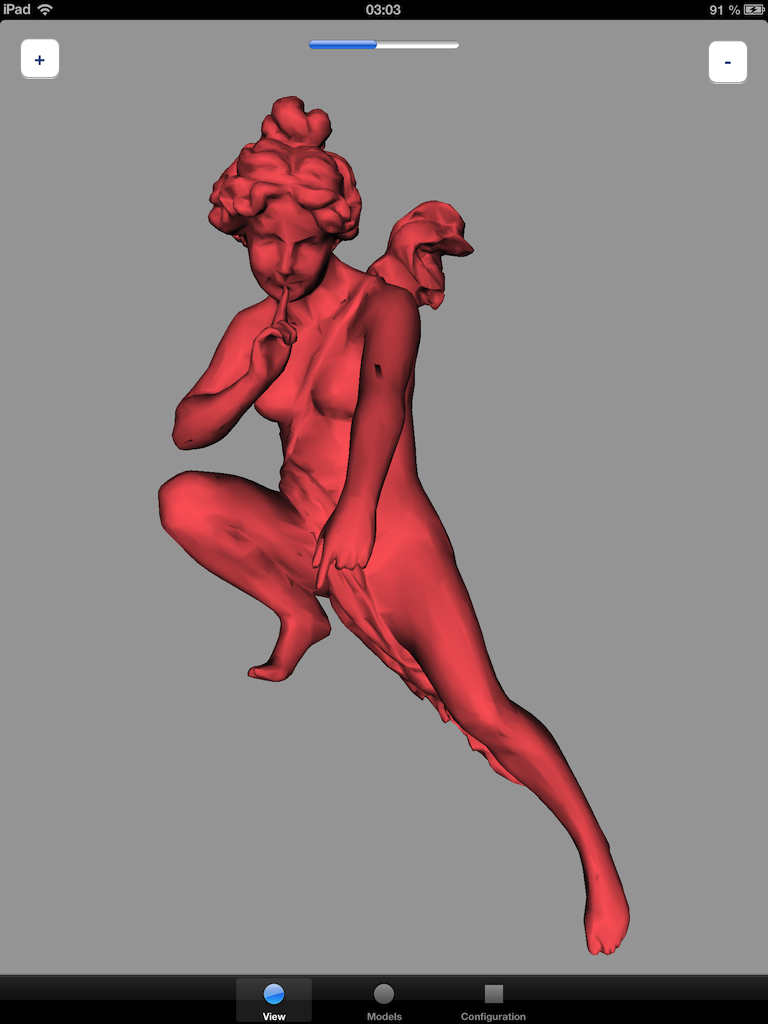
\includegraphics[width =0.45\textwidth] {results/030333.png}
	\label{fig:angel_visual_effects_2}
}

\subfigure[b][]{
	\centering
	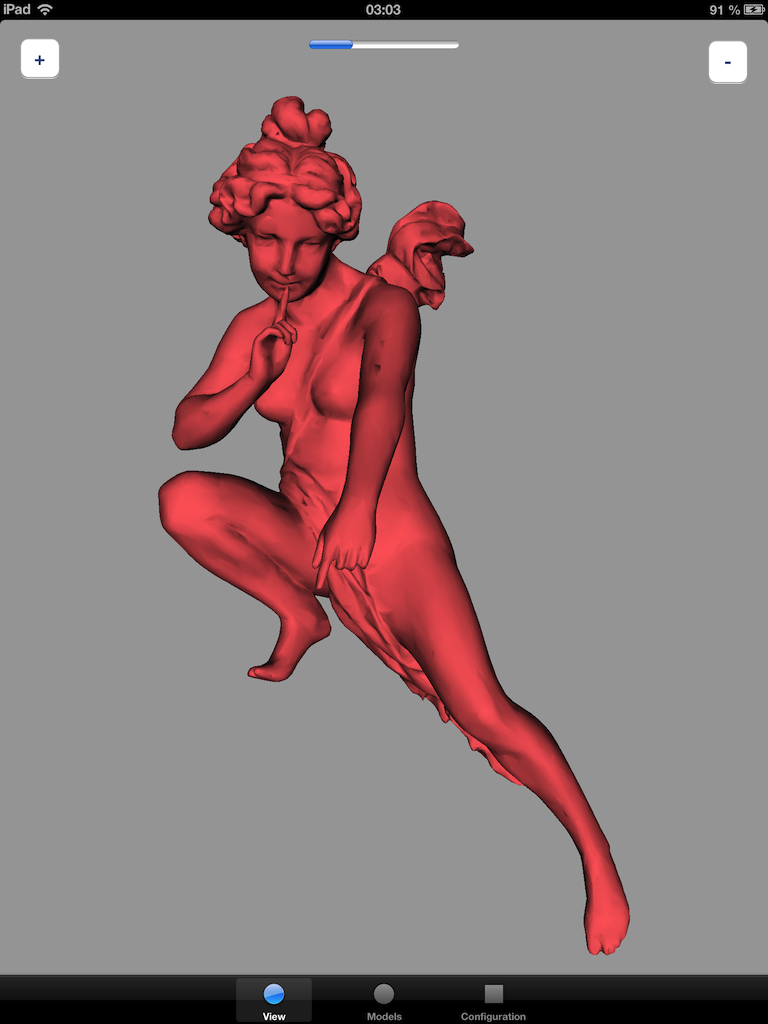
\includegraphics[width =0.45\textwidth] {results/030337.png}
	\label{fig:angel_visual_effects_3}
}
\hfill
\subfigure[b][]{
	\centering
	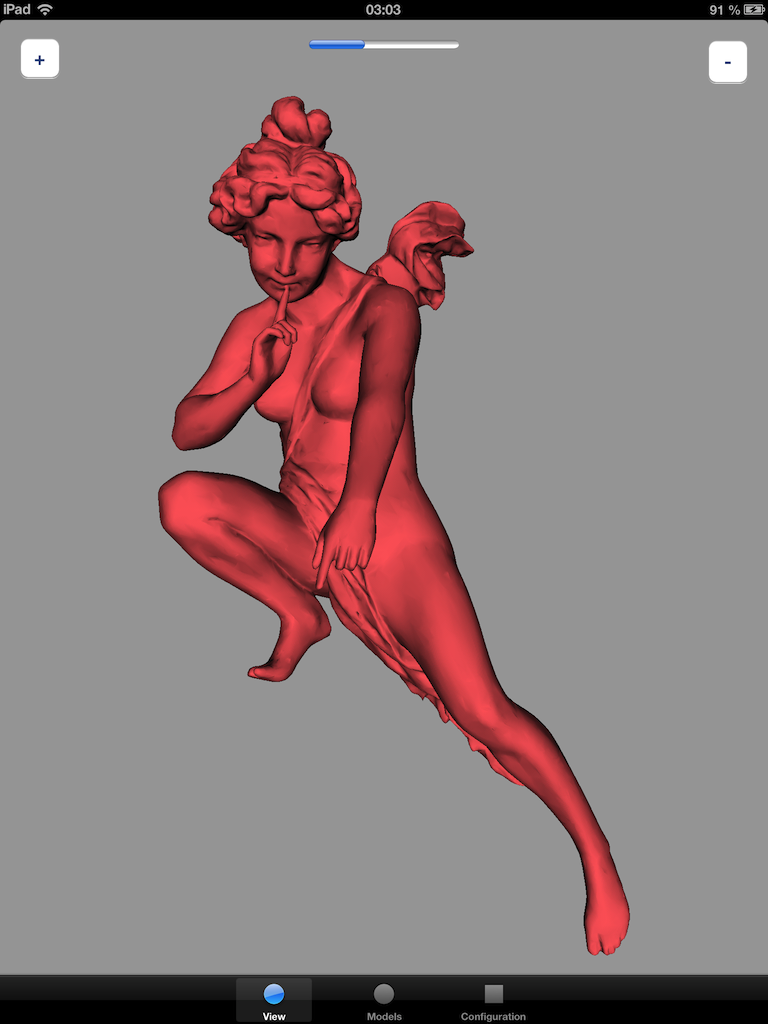
\includegraphics[width =0.45\textwidth] {results/030348.png}
	\label{fig:angel_visual_effects_4}
}

\label{fig:angel_visual_effects}
\caption{Visual Effects of Model "angel"}

\end{figure}

\begin{figure}
\centering

\subfigure[b][]{
	\centering
	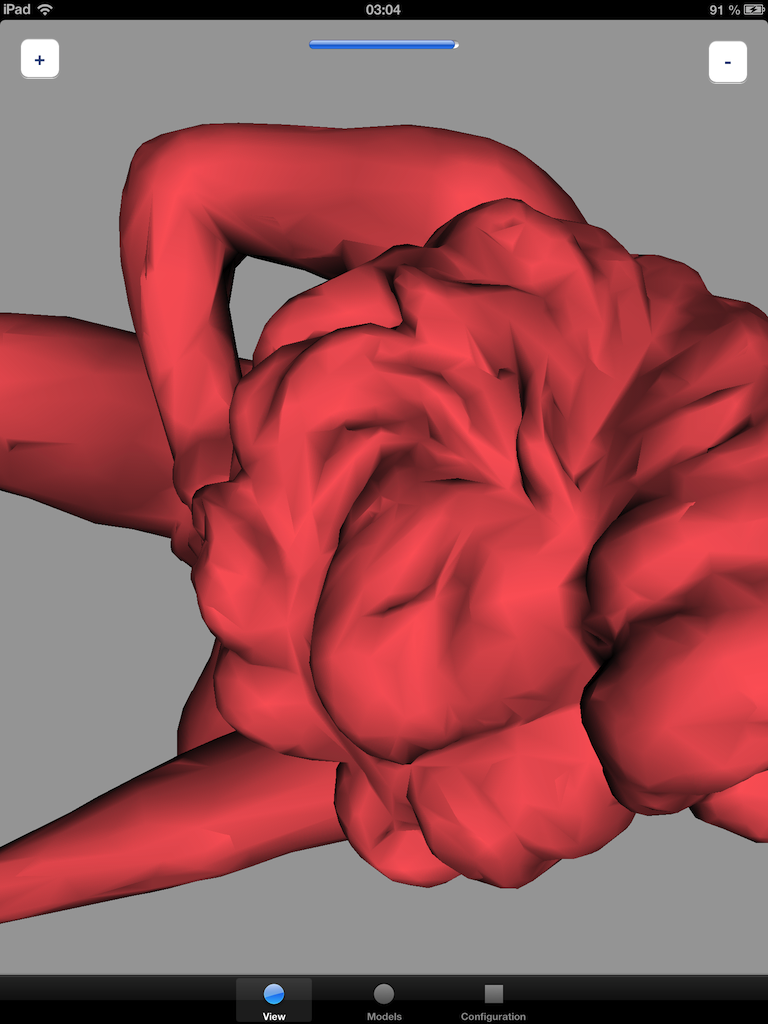
\includegraphics[width =0.45\textwidth] {results/030442.png}
	\label{fig:angel_visual_effects_hair2}
}
\hfill
\subfigure[b][]{
	\centering
	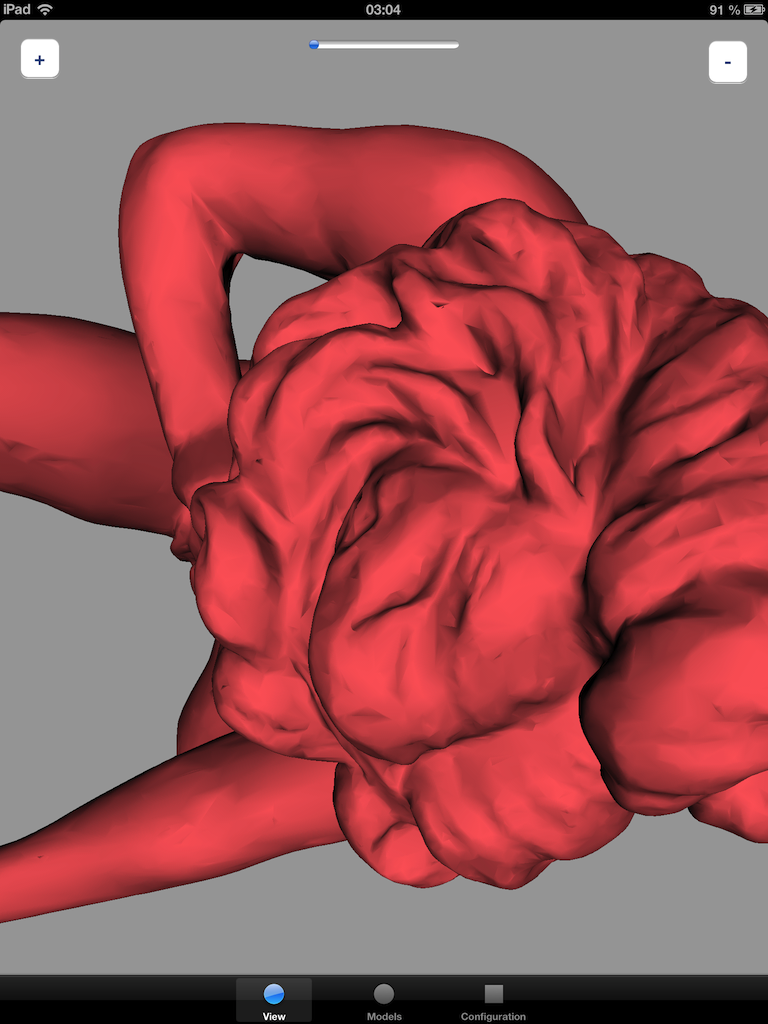
\includegraphics[width =0.45\textwidth] {results/030459.png}
	\label{fig:angel_visual_effects_hair4}
}

\subfigure[b][]{
	\centering
	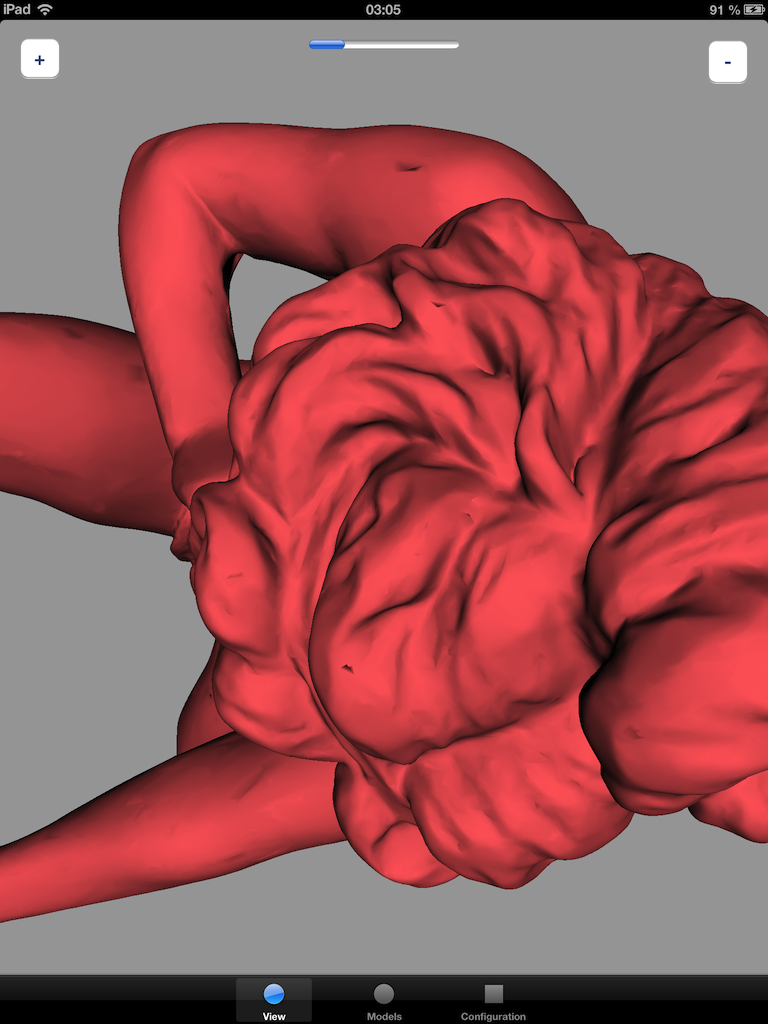
\includegraphics[width =0.45\textwidth] {results/030519.png}
	\label{fig:angel_visual_effects_hair6}
}
\hfill
\subfigure[b][]{
	\centering
	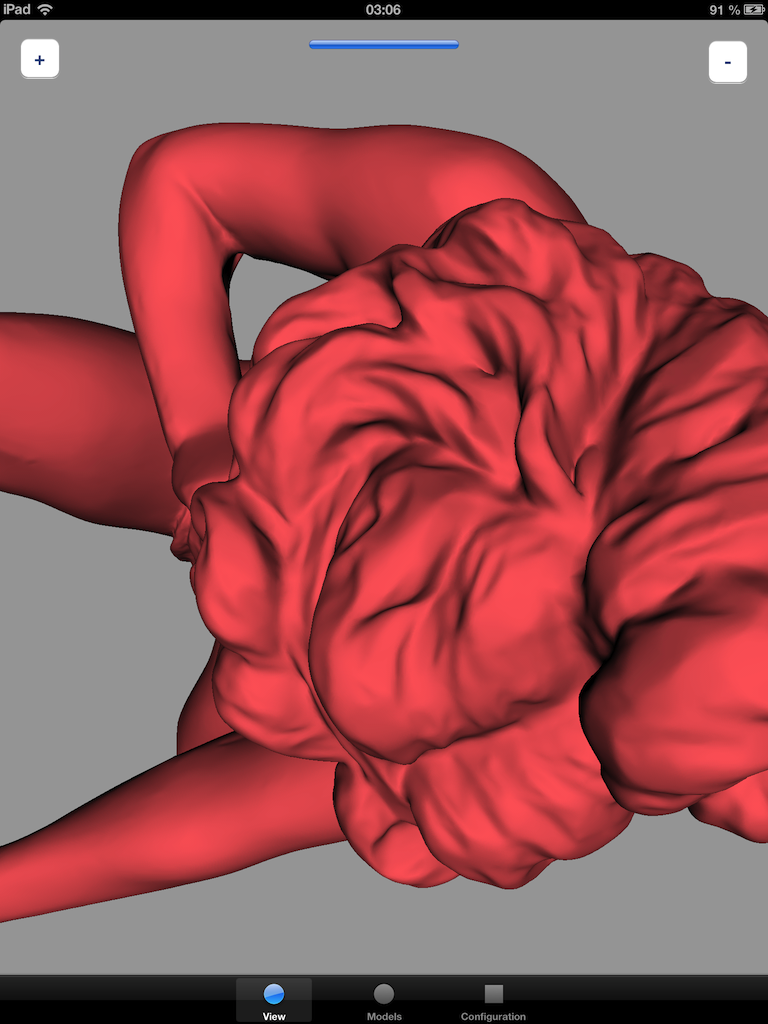
\includegraphics[width =0.45\textwidth] {results/030607.png}
	\label{fig:angel_visual_effects_hair8}
}

\label{fig:angel_visual_effects_hair}
\caption{Visual Effects of Model "angel"'s "hair"}
\end{figure}
When the client side starts to stream a mesh, it will be viewed on the client screen and refined on-the-fly, which means it can be seen as a refinement animation. Therefore we choose to illustrate this process in a sequence of screen shots using the model "angel". 







\subsection{Server Rendering Evaluation}
\label{section:servereva}
\begin{figure}
\centering
\subfigure[b][Size of Data Transfer. For each viewing param sync request, an image will be rendered in corresponding LOD and transmitted to client. We can see that the time of server side refinement and rendering is quite stable and the accumulative size of data transmitted are linearly increasing, as expected.]{
	\centering
	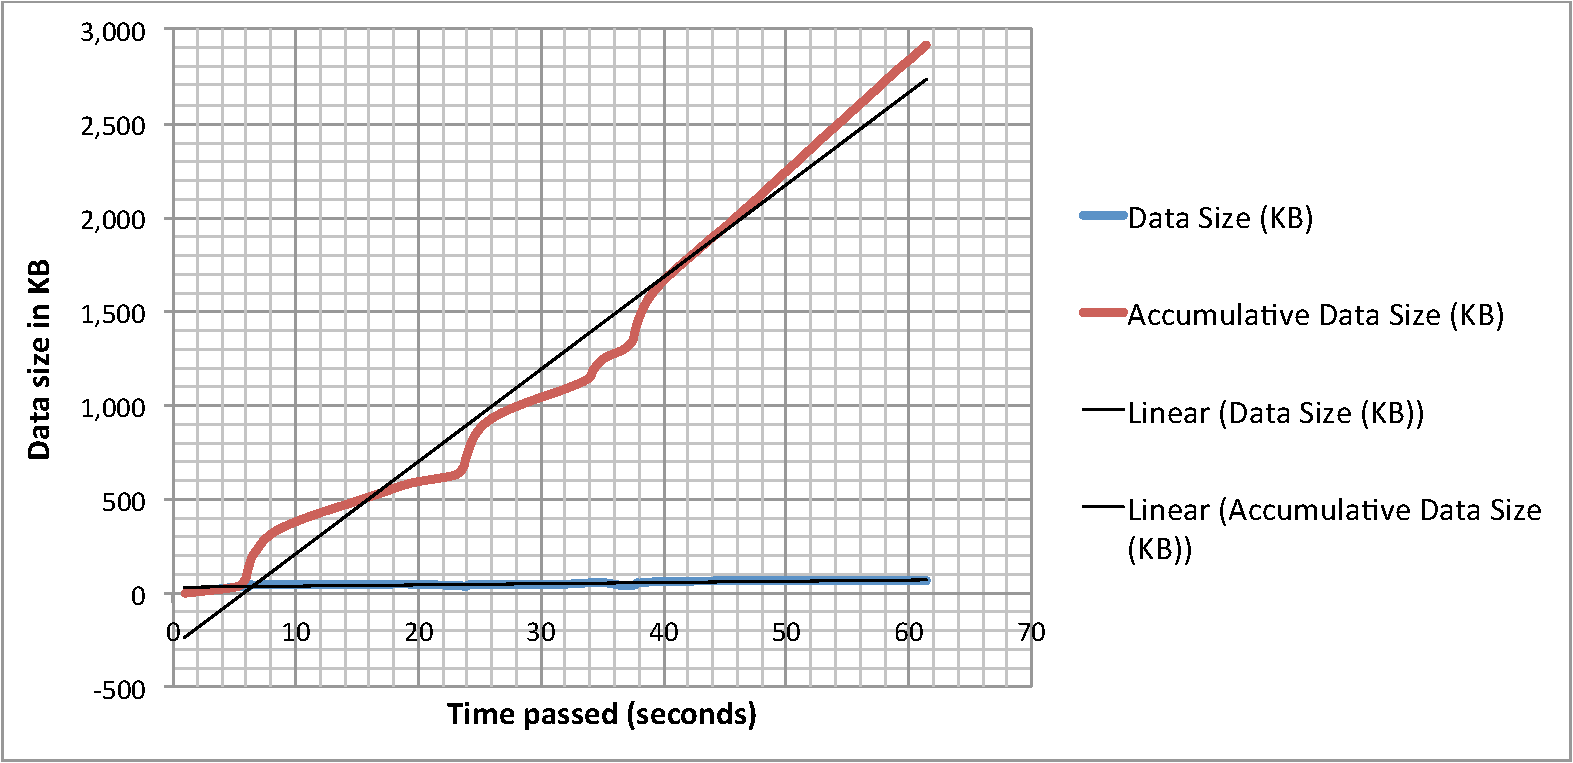
\includegraphics[width =\textwidth] {results/hapy_vrip_trans_datasize.pdf}
	\label{fig:hapy_vrip_svr_data_trans_datasize}
}
\subfigure[b][Num. of active vertices and faces of the server-hold model during streaming. The low points in the middle of the graph indicates the user is changing view and unnecessary edges are collapsed, unnecessary vertices are eliminated.]{
	\centering
	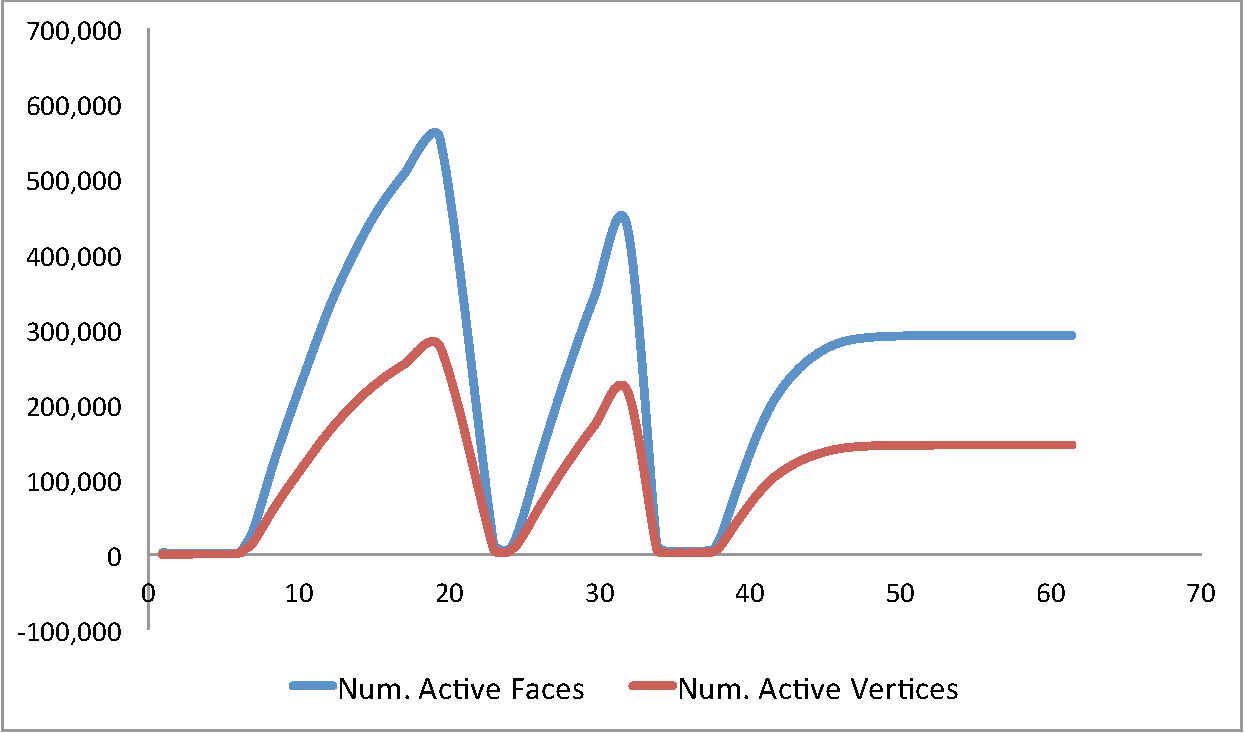
\includegraphics[width =\textwidth] {results/hapy_vrip_vfront_over_time.pdf}
	\label{fig:hapy_vrip_svr_data_trans_active_faces_vertices}
}
\label{fig:hapy_vrip_svr_data_trans}
\caption{Server Rendering Data Transmission Statistics of model "hapy\_vrip"}
\end{figure}
\begin{figure}
\centering
\subfigure[b][Data Transmission. X Axis: time (second), Y Axis: Data (KB).]{
	\centering
	\includegraphics[height=0.3\textheight] {results/thai_trans_data_perf.pdf}
	\label{fig:thai_trans_data}
}
\subfigure[b][Number of vertices and faces of the model refined during streaming. X Axis: Vertices/Faces Number, Y Axis: Time (second)]{
	\centering
	\includegraphics[height=0.3\textheight] {results/thai_trans_geo_perf.pdf}
	\label{fig:thai_trans_geo}
}

\subfigure[b][Number of vertices and faces of the model refined during streaming compared with time elapsed.]{
	\centering
	\includegraphics[height=0.3\textheight] {results/thai_trans_vft.pdf}
	\label{fig:thai_trans_vft}
}
\label{fig:thai_trans_perf}
\caption{Experiment results of model Thai Statue of 10 million triangles.}
\end{figure}



The server rendering evaluation experiments are performed on the models listed in \TA{table:modelsserverrendering}.

\subsubsection{Transmission Performance}
\label{section:servertransperf}
Since in the server rendering situation, both the refinement and rendering is done by the server, the definition of elapsed time becomes: $Time_{refinement}+Time_{rendering}+Time_{transmission}$. We choose the model "hapy\_vrip" for experiment. Details see \FG{fig:hapy_vrip_svr_data_trans_datasize} and \FG{fig:hapy_vrip_svr_data_trans_active_faces_vertices}. We can see that the server rendering of big meshes is quite fast. 

Moreover, we also did some experiments on more powerful workstations with larger models. We did server rendering experiment on the model Thai Statue from Stanford Scanning Repository, which has 10M faces. As showed in \FG{fig:thai_trans_data}, the data transferred in each request is stable since the server is just streaming images. \FG{fig:thai_trans_geo} shows the geometry statistics during streaming. And \FG{fig:thai_trans_vft} shows the geometry statistics compared with elapsed time of each request. Hypothetically the elapsed time should has linear relationship with the number of vertices and faces refined. However, it is interesting to find that there are two high points of elapsed time in the chart and their corresponding number of faces and vertices are relatively low. The reason of this is that during the time of those two high points, user has interrupted the refinement and rendering and is changing his view. And meanwhile, the server is deleting unnecessary geometry of the model. 


\subsubsection{Visual Quality}
\label{section:servervisualquality}

\begin{figure}
\centering
\subfigure[b][Visual Effects at low LOD level]{
	\centering
	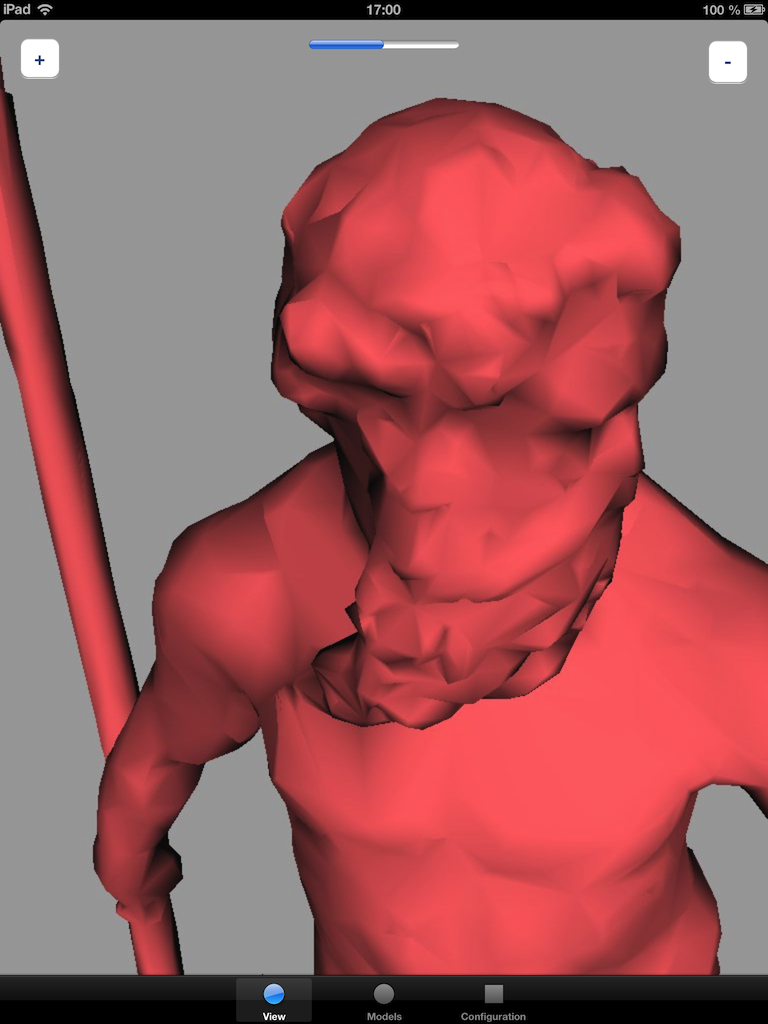
\includegraphics[width =0.3\textwidth] {results/170035.png}
	\label{fig:neptune_serverrendering_visual_effects1}
}
\hfill
\subfigure[b][Visual Effects at medium LOD level]{
	\centering
	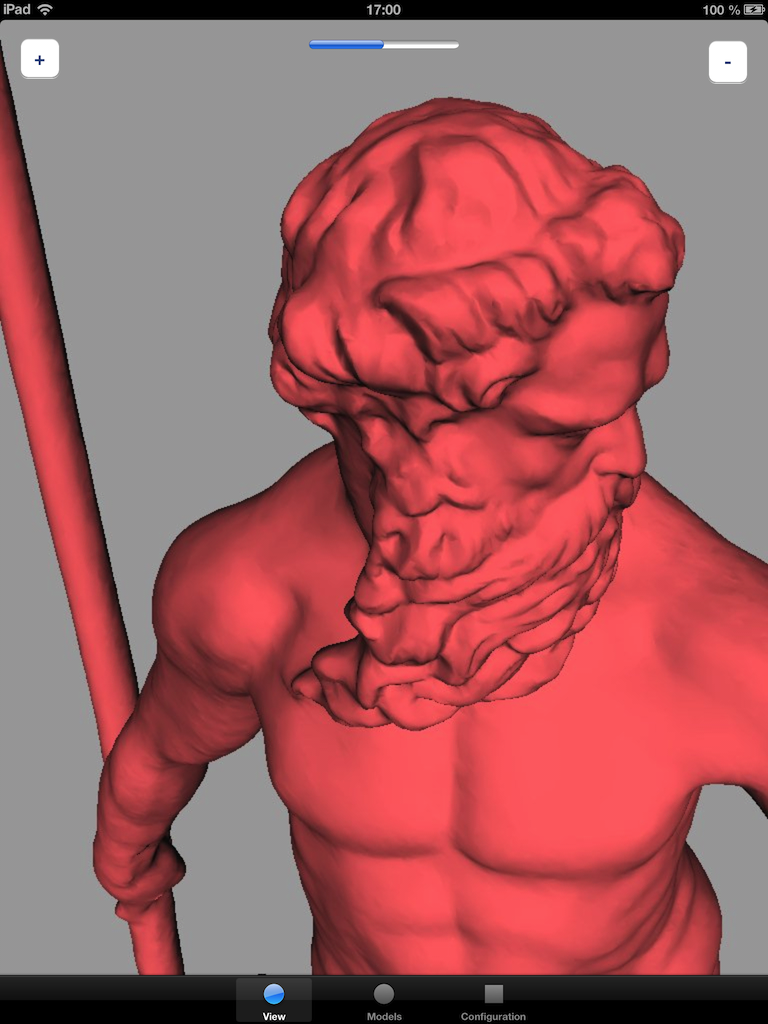
\includegraphics[width =0.3\textwidth] {results/170038.png}
	\label{fig:neptune_serverrendering_visual_effects2}
}
\hfill
\subfigure[b][Visual Effects at high LOD level]{
	\centering
	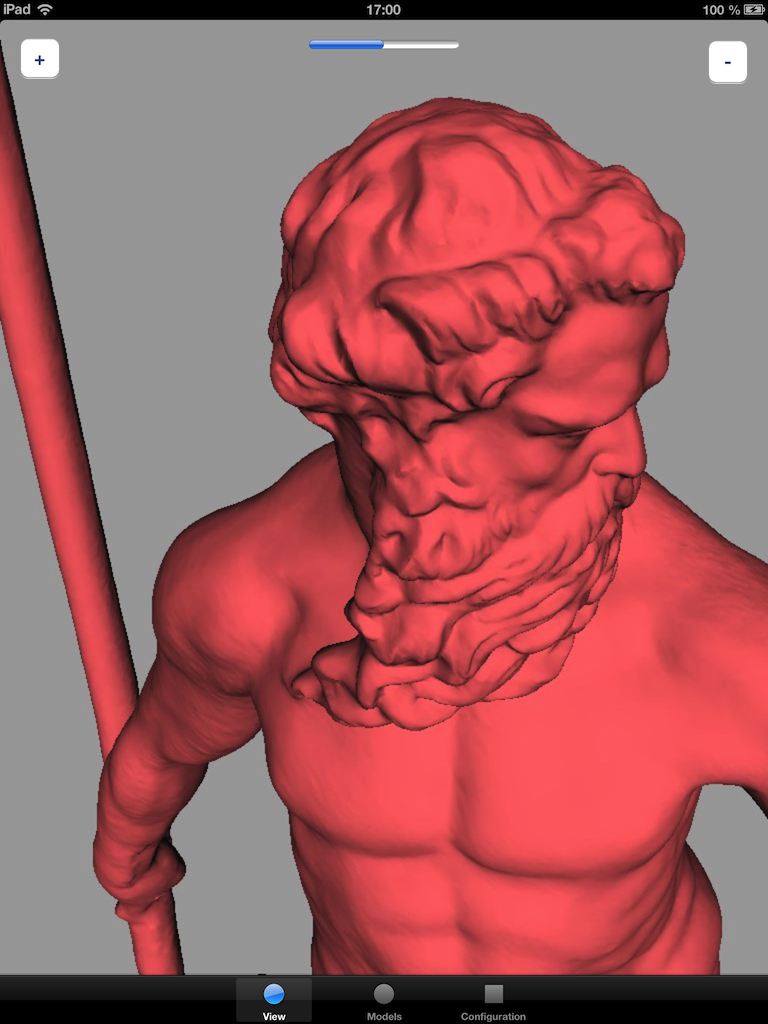
\includegraphics[width =0.3\textwidth] {results/170041.png}
	\label{fig:neptune_serverrendering_visual_effects3}
}

\label{fig:neptune_serverrendering_visual_effects}
\caption{Server Rendering Visual Effects of model "neptune" with 4M triangles}
\end{figure}


\begin{figure}
\centering
\subfigure[b][Visual Effects at low LOD level]{
	\centering
	\includegraphics[width =0.3\textwidth] {results/Thai_1.png}
	\label{fig:thai_serverrendering_visual_effects1}
}
\hfill
\subfigure[b][Visual Effects at medium LOD level]{
	\centering
	\includegraphics[width =0.3\textwidth] {results/Thai_2.png}
	\label{fig:thai_serverrendering_visual_effects2}
}
\hfill
\subfigure[b][Visual Effects at high LOD level]{
	\centering
	\includegraphics[width =0.3\textwidth] {results/Thai_3.png}
	\label{fig:Thai_serverrendering_visual_effects3}
	}
\subfigure[b][Visual Effects at low LOD level]{
	\centering
	\includegraphics[width =0.3\textwidth] {results/Thai_4.png}
	\label{fig:thai_serverrendering_visual_effects4}
}
\hfill
\subfigure[b][Visual Effects at medium LOD level]{
	\centering
	\includegraphics[width =0.3\textwidth] {results/Thai_5.png}
	\label{fig:thai_serverrendering_visual_effects5}
}
\hfill
\subfigure[b][Visual Effects at high LOD level]{
	\centering
	\includegraphics[width =0.3\textwidth] {results/Thai_6.png}
	\label{fig:thai_serverrendering_visual_effects6}
}

\label{fig:thai_serverrendering_visual_effects}
\caption{Server Rendering Visual Effects of model "Thai Statue" with 10M triangles}
\end{figure}

Similar to \SC{section:clientvisualquality}, in this section we will illustrate some screen shots to show the visual quality of server rendering streaming. It can be found that there is significant different between \FG{fig:neptune_serverrendering_visual_effects1} and \FG{fig:neptune_serverrendering_visual_effects2}, while \FG{fig:neptune_serverrendering_visual_effects2} and \FG{fig:neptune_serverrendering_visual_effects3} looks almost the same. So as the visual effects showed in \FG{fig:thai_serverrendering_visual_effects1} to \FG{fig:thai_serverrendering_visual_effects6}This is because when model's LOD reaches a certain high level, the triangles reconstructed could even be smaller than a pixel on screen, thus making it looks no difference compared with lower LOD level. 

\section{Discussion}
\label{section:results:discussion}
%\TODO{Discussion of test results. }
In the previous paragraphs, we have illustrated the result of experiment on our framework. It can be found that for both client and server rendering scenario, our framework is able to provide stable functionality of view-dependent progressive mesh streaming with high visual quality and performance. \\

In the scenario of client rendering, the performance bottleneck is mainly the client side since the model will finally reconstructed and rendered by the client and meanwhile the client has to support interruptible user interaction during refinement and rendering. On the other hand, in the scenario of server rendering, performance burden on client is relatively light and the main performance bottleneck is in the server side. The server needs to do almost every thing including refinement and rendering. And the client just have to show the rendered images from server. \\ 


%Picture
%\noindent
%\begin{minipage}{\linewidth}
%\makebox[\linewidth]{%
%\includegraphics[width=1.0\textwidth]{images/morphable.pdf}}
%\captionof{figure}{MorphableUI generates user-tailored interfaces for arbitrary applications in arbitrary environments. Users are able to use all available devices to control as many applications as needed. User behavior is analyzed by the system to increase the user experience.}% only if needed
%\label{fig:morphable}
%\bigskip
%\end{minipage}



%\chapter{Collaboration with Other Projects}
\label{chapter:Collaboration with Other Projects}
\TODO{In this chapter we will introduce the collaboration with other projects. Especially with the Hybrid Rendering Server Project.}



%Picture
%\noindent
%\begin{minipage}{\linewidth}
%\makebox[\linewidth]{%
%\includegraphics[width=1.0\textwidth]{images/morphable.pdf}}
%\captionof{figure}{MorphableUI generates user-tailored interfaces for arbitrary applications in arbitrary environments. Users are able to use all available devices to control as many applications as needed. User behavior is analyzed by the system to increase the user experience.}% only if needed
%\label{fig:morphable}
%\bigskip
%\end{minipage}



\chapter{Conclusion}
\label{chapter:Conclusion}
\TODO{Conclusion of this project. Recap the contribution. }
\section{Future Work}
\TODO{Discuss potential future work. like discussion of Quadric Error metrics ... advantage and disadvantage}



%Picture
%\noindent
%\begin{minipage}{\linewidth}
%\makebox[\linewidth]{%
%\includegraphics[width=1.0\textwidth]{images/morphable.pdf}}
%\captionof{figure}{MorphableUI generates user-tailored interfaces for arbitrary applications in arbitrary environments. Users are able to use all available devices to control as many applications as needed. User behavior is analyzed by the system to increase the user experience.}% only if needed
%\label{fig:morphable}
%\bigskip
%\end{minipage}










%%%
%%% end main document
%%%
%%%%%%%%%%%%%%%%%%%%%%%%%%%%%%%%%%%%%%%%%%%%%%%%%%%%%%%%%%%%%%%%%%%%%%%%%%%%%%%%

\appendix  %% include it, if something (bibliography, index, ...) follows below

%%%%%%%%%%%%%%%%%%%%%%%%%%%%%%%%%%%%%%%%%%%%%%%%%%%%%%%%%%%%%%%%%%%%%%%%%%%%%%%%
%%%
%%% bibliography
%%%
%%% available styles: abbrv, acm, alpha, apalike, ieeetr, plain, siam, unsrt
%%%
\bibliographystyle{acm}
%\bibliographystyle{alpha}
%\bibliographystyle{apalike}

%%% name of the bibliography file without .bib
%%% e.g.: literatur.bib -> \bibliography{literatur}
\bibliography{thesis}
\end{spacing}
\end{document}
%%% }}}
%%% END OF FILE
%%%%%%%%%%%%%%%%%%%%%%%%%%%%%%%%%%%%%%%%%%%%%%%%%%%%%%%%%%%%%%%%%%%%%%%%%%%%%%%%
%%% Notice!
%%% This file uses the outline-mode of emacs and the foldmethod of Vim.
%%% Press 'zi' to unfold the file in Vim.
%%% See ':help folding' for more information.
%%%%%%%%%%%%%%%%%%%%%%%%%%%%%%%%%%%%%%%%%%%%%%%%%%%%%%%%%%%%%%%%%%%%%%%%%%%%%%%%
%% Local Variables:
%% mode: outline-minor
%% OPToutline-regexp: "%% .*"
%% OPTeval: (hide-body)
%% emerge-set-combine-versions-template: "%a\n%b\n"
%% End:
%% vim:foldmethod=marker

